\subsubsection{simulateRandom} \label{sec:simulateRandom}

The operation \operator{simulateRandom} simulates a dynamic system for multiple random initial states $x_0 \in \mathcal{X}_0$ and random values for the inputs $u(t) \in \mathcal{U}$ as well as parameters $p \in \mathcal{P}$. The syntax is as follows:
\begin{equation*}
	\texttt{simRes} = \texttt{simulateRandom}(\texttt{sys},\texttt{params},\texttt{options})
\end{equation*}	
with input arguments
\begin{center}
\renewcommand{\arraystretch}{1.3}
\begin{tabular}[t]{l p{13cm} }
	$\bullet$~\texttt{sys} &  dynamic system defined by one of the classes in \cref{sec:continuousDynamics,sec:hybridDynamics}, e.g., \texttt{linearSys}, \texttt{hybridAutomaton}, etc. \\
	$\bullet$~\texttt{params} & struct containing the parameters that define the reachability problem. The parameters are identical to those for the operation \operator{reach} (see \cref{sec:reach}). \\
	$\bullet$~\texttt{options} & struct containing settings for the random simulation \\
		& \begin{tabular}[t]{l p{10cm}}	
		--~\texttt{.points} & number of random initial states (positive integer)\\
	 	--~\texttt{.type} & sampling method: \texttt{'standard'} (default, undefined distribution), \texttt{'gaussian'} (Gaussian distribution), \texttt{'rrt'} (sampling using \textit{rapidly exploring random trees})
	 	\end{tabular} \\
	 	& depending on the sampling method, there are different additional settings \\
		& \texttt{.type = 'standard'}: standard sampling method (undefined distribution) \\
		& \begin{tabular}[t]{l p{10cm}}	
	 	--~\texttt{.fracVert} & percentage of initial states randomly drawn from the vertices of the initial set $\mathcal{X}_0$ (value in $[0,1]$) \\ 	
	 	--~\texttt{.fracInpVert} & percentage of input values randomly drawn from the vertices of the input set $\mathcal{U}$ (value in $[0,1]$) \\
	 	--~\texttt{.nrConstInp} & number piecewise-constant input values within the input signal during simulation (integer $\geq 1$) \\
	 	\end{tabular} \\
	 	& \texttt{.type = 'rrt'}: sampling using \emph{rapidly-exploring random trees} \\
	 	& \begin{tabular}[t]{l p{10cm}}	
	 	--~\texttt{.vertSamp} & flag specifying whether random initial states, inputs, and parameters are sampled from the vertices of the corresponding sets (0 or 1).\\ 	
	 	--~\texttt{.stretchFac} & stretching factor for enlarging the reachable sets during execution of the algorithm (scalar $>$ 1). \\
	 	--~\texttt{.R} & object of class \texttt{reachSet} (see \cref{sec:reachSet}) that stores the reachable set for the corresponding reachability problem.
	 	\end{tabular} \\
	 	& \texttt{.type = 'gaussian'}: sampling from gaussian distribution \\
		& \begin{tabular}[t]{l p{10cm}}	
	 	--~\texttt{.nrConstInp} & number piecewise-constant input values within the input signal during simulation (integer $\geq 1$) \\
	 	--~\texttt{.p\_conf} & probability that sampled value is within the set (value in $(0,1)$)
	 	\end{tabular}
\end{tabular}
\end{center}

and output arguments

\begin{center}
\renewcommand{\arraystretch}{1.3}
\begin{tabular}[t]{l p{13cm} }
	$\bullet$~\texttt{simRes} & object of class \texttt{simResult} (see \cref{sec:simResult}) that stores the simulated trajectories.
\end{tabular}
\end{center}

Let us demonstrate the operation \texttt{simulateRandom} by an example:

\begin{center}
\begin{minipage}[t]{0.58\textwidth}
	\footnotesize
	% This file was created by matlab2tikz.
%
\definecolor{mycolor1}{rgb}{0.27060,0.58820,1.00000}%
%
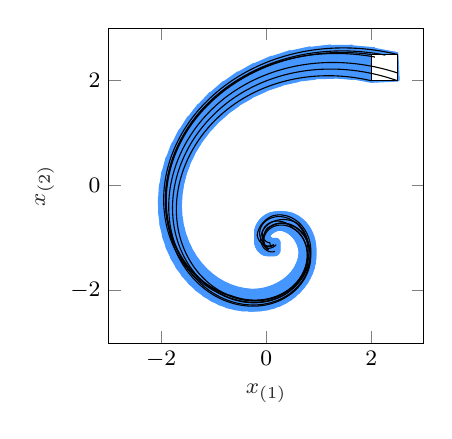
\begin{tikzpicture}
\footnotesize

\begin{axis}[%
width=4cm,
height=4cm,
at={(0in,0in)},
scale only axis,
xmin=-3,
xmax=3,
xlabel style={font=\color{white!15!black}},
xlabel={$x_{(1)}$},
ymin=-3,
ymax=3,
ylabel style={font=\color{white!15!black}},
ylabel={$x_{(2)}$},
axis background/.style={fill=white}
]

\addplot[area legend, draw=mycolor1, fill=mycolor1, forget plot]
table[row sep=crcr] {%
x	y\\
2.0015	1.9698\\
2.0079	1.9698\\
2.4981	1.9939\\
2.5222	2.0037\\
2.5324	2.0139\\
2.5324	2.0207\\
2.5083	2.5109\\
2.4985	2.535\\
2.4983	2.5352\\
2.4976	2.5356\\
2.0968	2.6103\\
2.0905	2.6103\\
1.6003	2.5862\\
1.5762	2.5764\\
1.5659	2.5661\\
1.5659	2.5594\\
1.59	2.0692\\
1.5998	2.0451\\
1.6001	2.0448\\
1.6007	2.0445\\
2.0015	1.9698\\
}--cycle;

\addplot[area legend, draw=mycolor1, fill=mycolor1, forget plot]
table[row sep=crcr] {%
x	y\\
1.6328	2.0264\\
1.6378	2.0269\\
1.6389	2.027\\
2.1076	2.0974\\
2.1298	2.1091\\
2.1398	2.1191\\
2.14	2.1194\\
2.1486	2.1299\\
2.1481	2.135\\
2.148	2.1365\\
2.0776	2.6051\\
2.0658	2.6273\\
2.0656	2.6276\\
2.0649	2.6279\\
2.0642	2.6281\\
1.672	2.6613\\
1.667	2.6608\\
1.6659	2.6607\\
1.1972	2.5903\\
1.175	2.5785\\
1.1648	2.5683\\
1.1561	2.5577\\
1.1566	2.5527\\
1.1568	2.5512\\
1.2272	2.0825\\
1.2389	2.0603\\
1.2392	2.0601\\
1.2399	2.0598\\
1.2405	2.0595\\
1.6328	2.0264\\
}--cycle;

\addplot[area legend, draw=mycolor1, fill=mycolor1, forget plot]
table[row sep=crcr] {%
x	y\\
0.893	2.0392\\
1.2731	2.0452\\
1.2779	2.0461\\
1.2789	2.0464\\
1.7224	2.1592\\
1.7426	2.1726\\
1.7526	2.1826\\
1.7612	2.1932\\
1.7614	2.1934\\
1.7687	2.2044\\
1.7687	2.2045\\
1.7678	2.2093\\
1.7675	2.2107\\
1.6547	2.6541\\
1.6412	2.6744\\
1.641	2.6745\\
1.6403	2.6749\\
1.6389	2.6753\\
1.2588	2.6693\\
1.2541	2.6684\\
1.253	2.6682\\
0.8096	2.5553\\
0.7893	2.5419\\
0.7793	2.5319\\
0.7707	2.5213\\
0.7705	2.5211\\
0.7632	2.5101\\
0.7632	2.51\\
0.7642	2.5053\\
0.7645	2.5038\\
0.8773	2.0604\\
0.8907	2.0402\\
0.891	2.04\\
0.8917	2.0396\\
0.8923	2.0394\\
0.893	2.0392\\
}--cycle;

\addplot[area legend, draw=mycolor1, fill=mycolor1, forget plot]
table[row sep=crcr] {%
x	y\\
0.5611	1.9862\\
0.9257	2.0286\\
0.9267	2.0289\\
0.9312	2.0303\\
1.3464	2.1814\\
1.3645	2.1963\\
1.3745	2.2063\\
1.3831	2.2168\\
1.3904	2.2278\\
1.3906	2.2281\\
1.3965	2.2394\\
1.3951	2.2439\\
1.3947	2.2453\\
1.2436	2.6605\\
1.2287	2.6786\\
1.2285	2.6788\\
1.2278	2.6791\\
1.2264	2.6795\\
1.2258	2.6796\\
0.8611	2.6372\\
0.8602	2.6369\\
0.8557	2.6355\\
0.4405	2.4844\\
0.4223	2.4695\\
0.4123	2.4595\\
0.4037	2.449\\
0.3964	2.438\\
0.3963	2.4377\\
0.3903	2.4265\\
0.3903	2.4264\\
0.3917	2.4219\\
0.3921	2.4206\\
0.5433	2.0053\\
0.5581	1.9872\\
0.5584	1.9871\\
0.5591	1.9867\\
0.5597	1.9865\\
0.5604	1.9863\\
0.5611	1.9862\\
}--cycle;

\addplot[area legend, draw=mycolor1, fill=mycolor1, forget plot]
table[row sep=crcr] {%
x	y\\
0.2473	1.9033\\
0.5935	1.9792\\
0.5977	1.9809\\
0.5986	1.9813\\
0.9829	2.1666\\
1.0089	2.1926\\
1.0176	2.2031\\
1.0249	2.2141\\
1.0308	2.2254\\
1.0309	2.2257\\
1.0355	2.2371\\
1.0338	2.2413\\
1.0333	2.2426\\
0.848	2.6269\\
0.832	2.6429\\
0.8313	2.6432\\
0.831	2.6434\\
0.8304	2.6436\\
0.8297	2.6438\\
0.829	2.6439\\
0.8284	2.6439\\
0.4821	2.5681\\
0.478	2.5663\\
0.4771	2.5659\\
0.0927	2.3807\\
0.0667	2.3547\\
0.0581	2.3441\\
0.0508	2.3331\\
0.0448	2.3218\\
0.0447	2.3216\\
0.0401	2.3102\\
0.0401	2.3101\\
0.0419	2.3059\\
0.0424	2.3046\\
0.2276	1.9203\\
0.2436	1.9043\\
0.2443	1.904\\
0.2446	1.9039\\
0.2453	1.9036\\
0.246	1.9034\\
0.2466	1.9033\\
0.2473	1.9033\\
}--cycle;

\addplot[area legend, draw=mycolor1, fill=mycolor1, forget plot]
table[row sep=crcr] {%
x	y\\
-0.0469	1.7934\\
-0.0462	1.7934\\
0.2791	1.8996\\
0.2829	1.9017\\
0.2838	1.9022\\
0.6352	2.1172\\
0.6452	2.1272\\
0.6539	2.1378\\
0.6677	2.1547\\
0.6749	2.1657\\
0.6809	2.177\\
0.6855	2.1884\\
0.6856	2.1886\\
0.6889	2.2\\
0.6889	2.2001\\
0.6868	2.204\\
0.6862	2.2051\\
0.4712	2.5566\\
0.4543	2.5704\\
0.4529	2.571\\
0.4526	2.5711\\
0.452	2.5712\\
0.4506	2.5714\\
0.45	2.5713\\
0.1247	2.4651\\
0.1208	2.463\\
0.12	2.4625\\
-0.2314	2.2475\\
-0.2414	2.2375\\
-0.2501	2.2269\\
-0.2639	2.21\\
-0.2712	2.199\\
-0.2771	2.1877\\
-0.2817	2.1763\\
-0.2818	2.1761\\
-0.2852	2.1647\\
-0.2852	2.1646\\
-0.2831	2.1607\\
-0.2824	2.1596\\
-0.0674	1.8081\\
-0.0505	1.7943\\
-0.0498	1.794\\
-0.0491	1.7938\\
-0.0489	1.7937\\
-0.0482	1.7935\\
-0.0475	1.7934\\
-0.0469	1.7934\\
}--cycle;

\addplot[area legend, draw=mycolor1, fill=mycolor1, forget plot]
table[row sep=crcr] {%
x	y\\
-0.3189	1.6594\\
-0.3182	1.6594\\
-0.3176	1.6595\\
-0.0153	1.7929\\
-0.0118	1.7953\\
-0.011	1.7958\\
0.3059	2.0363\\
0.3159	2.0463\\
0.3245	2.0569\\
0.3318	2.0679\\
0.3434	2.0855\\
0.3494	2.0967\\
0.354	2.1081\\
0.3573	2.1195\\
0.3574	2.1198\\
0.3595	2.1311\\
0.3595	2.1312\\
0.3571	2.1347\\
0.3564	2.1357\\
0.1159	2.4526\\
0.0983	2.4643\\
0.0977	2.4646\\
0.097	2.4649\\
0.0963	2.465\\
0.096	2.4651\\
0.0954	2.4652\\
0.0941	2.4652\\
0.0935	2.4651\\
-0.2089	2.3316\\
-0.2123	2.3293\\
-0.2131	2.3287\\
-0.53	2.0883\\
-0.54	2.0783\\
-0.5487	2.0677\\
-0.556	2.0567\\
-0.5676	2.0391\\
-0.5735	2.0278\\
-0.5782	2.0165\\
-0.5815	2.0051\\
-0.5816	2.0048\\
-0.5837	1.9935\\
-0.5837	1.9934\\
-0.5813	1.9899\\
-0.5806	1.9888\\
-0.3401	1.6719\\
-0.3225	1.6603\\
-0.3211	1.6597\\
-0.3205	1.6596\\
-0.3202	1.6595\\
-0.3195	1.6594\\
-0.3189	1.6594\\
}--cycle;

\addplot[area legend, draw=mycolor1, fill=mycolor1, forget plot]
table[row sep=crcr] {%
x	y\\
-0.5673	1.5044\\
-0.5666	1.5044\\
-0.566	1.5045\\
-0.5655	1.5047\\
-0.2879	1.662\\
-0.2872	1.6626\\
-0.2841	1.6652\\
-0.0028	1.9268\\
0.0072	1.9368\\
0.0159	1.9474\\
0.0232	1.9584\\
0.0291	1.9697\\
0.0386	1.9877\\
0.0432	1.9991\\
0.0466	2.0105\\
0.0487	2.0217\\
0.0487	2.022\\
0.0497	2.033\\
0.0497	2.0332\\
0.047	2.0363\\
0.0462	2.0372\\
-0.2154	2.3185\\
-0.2334	2.328\\
-0.2341	2.3284\\
-0.2347	2.3286\\
-0.2354	2.3288\\
-0.2361	2.3289\\
-0.2377	2.3289\\
-0.2383	2.3288\\
-0.2388	2.3287\\
-0.5165	2.1713\\
-0.5171	2.1707\\
-0.5202	2.1681\\
-0.8015	1.9065\\
-0.8115	1.8965\\
-0.8202	1.8859\\
-0.8275	1.8749\\
-0.8334	1.8637\\
-0.8429	1.8457\\
-0.8475	1.8343\\
-0.8509	1.8229\\
-0.853	1.8116\\
-0.853	1.8113\\
-0.854	1.8003\\
-0.854	1.8002\\
-0.8513	1.797\\
-0.8505	1.7961\\
-0.5889	1.5148\\
-0.5709	1.5053\\
-0.5702	1.505\\
-0.5696	1.5047\\
-0.5682	1.5045\\
-0.568	1.5044\\
-0.5673	1.5044\\
}--cycle;

\addplot[area legend, draw=mycolor1, fill=mycolor1, forget plot]
table[row sep=crcr] {%
x	y\\
-0.7911	1.3316\\
-0.7904	1.3316\\
-0.7892	1.3318\\
-0.7887	1.332\\
-0.5371	1.51\\
-0.5265	1.5206\\
-0.5238	1.5234\\
-0.2787	1.8019\\
-0.2701	1.8125\\
-0.2628	1.8235\\
-0.2569	1.8347\\
-0.2522	1.8461\\
-0.2449	1.8643\\
-0.2415	1.8757\\
-0.2394	1.887\\
-0.2385	1.898\\
-0.2385	1.8985\\
-0.2386	1.9092\\
-0.2414	1.9119\\
-0.2423	1.9127\\
-0.5207	2.1578\\
-0.5214	2.1581\\
-0.5396	2.1655\\
-0.541	2.1659\\
-0.5416	2.166\\
-0.5433	2.166\\
-0.5439	2.1659\\
-0.5444	2.1658\\
-0.545	2.1656\\
-0.7965	1.9876\\
-0.8099	1.9742\\
-1.0549	1.6957\\
-1.0635	1.6851\\
-1.0708	1.6741\\
-1.0768	1.6629\\
-1.0814	1.6515\\
-1.0888	1.6333\\
-1.0921	1.6219\\
-1.0942	1.6106\\
-1.0952	1.5996\\
-1.0952	1.5991\\
-1.095	1.5884\\
-1.0922	1.5857\\
-1.0914	1.5849\\
-0.8129	1.3398\\
-0.8122	1.3395\\
-0.794	1.3321\\
-0.7933	1.3319\\
-0.7927	1.3317\\
-0.792	1.3316\\
-0.7911	1.3316\\
}--cycle;

\addplot[area legend, draw=mycolor1, fill=mycolor1, forget plot]
table[row sep=crcr] {%
x	y\\
-0.9903	1.1439\\
-0.9889	1.1439\\
-0.9887	1.144\\
-0.9881	1.144\\
-0.9875	1.1442\\
-0.9865	1.1446\\
-0.7619	1.3399\\
-0.7519	1.3499\\
-0.7433	1.3604\\
-0.7428	1.3611\\
-0.7404	1.364\\
-0.5318	1.6552\\
-0.5245	1.6662\\
-0.5186	1.6775\\
-0.514	1.6889\\
-0.5106	1.7002\\
-0.5053	1.7185\\
-0.5032	1.7297\\
-0.5023	1.7408\\
-0.5023	1.741\\
-0.5024	1.7517\\
-0.5024	1.752\\
-0.5036	1.7622\\
-0.5066	1.7646\\
-0.5075	1.7653\\
-0.7986	1.9739\\
-0.8	1.9745\\
-0.8182	1.9798\\
-0.8189	1.98\\
-0.8195	1.9801\\
-0.8209	1.9801\\
-0.8212	1.98\\
-0.8218	1.98\\
-0.8223	1.9798\\
-0.8229	1.9796\\
-0.8233	1.9794\\
-1.0479	1.7841\\
-1.0579	1.7741\\
-1.0665	1.7636\\
-1.067	1.7629\\
-1.0694	1.7599\\
-1.278	1.4688\\
-1.2853	1.4578\\
-1.2912	1.4465\\
-1.2959	1.4351\\
-1.2992	1.4238\\
-1.3045	1.4055\\
-1.3066	1.3943\\
-1.3076	1.3832\\
-1.3076	1.383\\
-1.3074	1.3723\\
-1.3074	1.372\\
-1.3062	1.3618\\
-1.3033	1.3594\\
-1.3024	1.3587\\
-1.0112	1.1501\\
-1.0105	1.1498\\
-1.0099	1.1495\\
-0.9916	1.1442\\
-0.991	1.144\\
-0.9903	1.1439\\
}--cycle;

\addplot[area legend, draw=mycolor1, fill=mycolor1, forget plot]
table[row sep=crcr] {%
x	y\\
-1.1634	0.9445\\
-1.1608	0.9445\\
-1.1605	0.9446\\
-1.16	0.9447\\
-1.1594	0.9449\\
-1.1589	0.9452\\
-1.1585	0.9454\\
-1.1485	0.9554\\
-0.9516	1.1646\\
-0.9429	1.1752\\
-0.9356	1.1862\\
-0.9337	1.1893\\
-0.9332	1.19\\
-0.7609	1.4898\\
-0.7549	1.5011\\
-0.7503	1.5125\\
-0.747	1.5239\\
-0.7449	1.5351\\
-0.7415	1.5532\\
-0.7405	1.5642\\
-0.7405	1.5647\\
-0.7407	1.5754\\
-0.7419	1.5856\\
-0.7419	1.5858\\
-0.744	1.5956\\
-0.745	1.5962\\
-0.748	1.5982\\
-1.0479	1.7705\\
-1.0486	1.7708\\
-1.0492	1.7711\\
-1.0499	1.7712\\
-1.0679	1.7746\\
-1.0708	1.7746\\
-1.0714	1.7744\\
-1.0724	1.774\\
-1.0729	1.7737\\
-1.0829	1.7637\\
-1.2798	1.5545\\
-1.2884	1.5439\\
-1.2957	1.5329\\
-1.2977	1.5298\\
-1.2981	1.5292\\
-1.4705	1.2293\\
-1.4764	1.2181\\
-1.481	1.2067\\
-1.4844	1.1953\\
-1.4865	1.184\\
-1.4899	1.166\\
-1.4908	1.155\\
-1.4908	1.1545\\
-1.4906	1.1438\\
-1.4895	1.1335\\
-1.4894	1.1333\\
-1.4873	1.1236\\
-1.4864	1.123\\
-1.4833	1.121\\
-1.1835	0.9486\\
-1.1828	0.9483\\
-1.1814	0.9479\\
-1.1634	0.9445\\
}--cycle;

\addplot[area legend, draw=mycolor1, fill=mycolor1, forget plot]
table[row sep=crcr] {%
x	y\\
-1.31	0.7363\\
-1.3066	0.7363\\
-1.3064	0.7364\\
-1.3054	0.7368\\
-1.3049	0.7371\\
-1.3045	0.7374\\
-1.2945	0.7474\\
-1.2859	0.758\\
-1.1169	0.978\\
-1.1096	0.989\\
-1.1036	1.0002\\
-1.102	1.0034\\
-1.1017	1.0041\\
-0.965	1.3088\\
-0.9604	1.3202\\
-0.957	1.3316\\
-0.9549	1.3428\\
-0.954	1.3539\\
-0.9525	1.3715\\
-0.9525	1.3828\\
-0.9537	1.3931\\
-0.9558	1.4028\\
-0.9558	1.403\\
-0.9588	1.4122\\
-0.962	1.4138\\
-0.9629	1.4143\\
-0.9636	1.4146\\
-1.2683	1.5513\\
-1.269	1.5515\\
-1.2696	1.5517\\
-1.2873	1.5532\\
-1.2907	1.5532\\
-1.2909	1.5531\\
-1.2919	1.5527\\
-1.2924	1.5524\\
-1.2928	1.5521\\
-1.3028	1.5421\\
-1.3114	1.5315\\
-1.4804	1.3116\\
-1.4877	1.3006\\
-1.4937	1.2893\\
-1.4956	1.2855\\
-1.6323	0.9807\\
-1.6369	0.9694\\
-1.6403	0.958\\
-1.6424	0.9467\\
-1.6433	0.9357\\
-1.6448	0.918\\
-1.6448	0.9067\\
-1.6436	0.8965\\
-1.6415	0.8867\\
-1.6415	0.8865\\
-1.6385	0.8773\\
-1.6353	0.8757\\
-1.6344	0.8753\\
-1.6337	0.8749\\
-1.329	0.7382\\
-1.3276	0.7378\\
-1.31	0.7363\\
}--cycle;

\addplot[area legend, draw=mycolor1, fill=mycolor1, forget plot]
table[row sep=crcr] {%
x	y\\
-1.4484	0.5219\\
-1.4438	0.5219\\
-1.4267	0.5222\\
-1.4265	0.5223\\
-1.426	0.5225\\
-1.4248	0.5234\\
-1.4148	0.5334\\
-1.4062	0.544\\
-1.3989	0.555\\
-1.2577	0.7826\\
-1.2518	0.7939\\
-1.2471	0.8053\\
-1.2469	0.806\\
-1.2456	0.8092\\
-1.1437	1.1151\\
-1.1403	1.1265\\
-1.1382	1.1378\\
-1.1373	1.1488\\
-1.1373	1.1605\\
-1.1375	1.1776\\
-1.1387	1.1878\\
-1.1408	1.1976\\
-1.1438	1.2067\\
-1.1439	1.2069\\
-1.1476	1.2154\\
-1.1483	1.2158\\
-1.1515	1.217\\
-1.1524	1.2174\\
-1.1531	1.2176\\
-1.4591	1.3196\\
-1.4637	1.3196\\
-1.4807	1.3193\\
-1.481	1.3192\\
-1.4815	1.319\\
-1.4827	1.3181\\
-1.4927	1.3081\\
-1.5013	1.2975\\
-1.5086	1.2865\\
-1.6498	1.0588\\
-1.6557	1.0476\\
-1.6603	1.0362\\
-1.6606	1.0355\\
-1.6619	1.0323\\
-1.7638	0.7264\\
-1.7671	0.715\\
-1.7693	0.7037\\
-1.7702	0.6927\\
-1.7702	0.681\\
-1.7699	0.6639\\
-1.7688	0.6536\\
-1.7666	0.6439\\
-1.7637	0.6348\\
-1.7636	0.6345\\
-1.7598	0.626\\
-1.7592	0.6257\\
-1.756	0.6245\\
-1.755	0.6241\\
-1.4484	0.5219\\
}--cycle;

\addplot[area legend, draw=mycolor1, fill=mycolor1, forget plot]
table[row sep=crcr] {%
x	y\\
-1.5437	0.3029\\
-1.5379	0.3029\\
-1.5215	0.3048\\
-1.5213	0.3049\\
-1.5208	0.3052\\
-1.5204	0.3055\\
-1.5101	0.3158\\
-1.5098	0.3162\\
-1.5011	0.3267\\
-1.4938	0.3377\\
-1.4879	0.349\\
-1.3742	0.5813\\
-1.3696	0.5927\\
-1.3662	0.6041\\
-1.3653	0.6073\\
-1.3651	0.608\\
-1.2967	0.9118\\
-1.2946	0.923\\
-1.2936	0.9341\\
-1.2936	0.9462\\
-1.2948	0.9565\\
-1.2967	0.9729\\
-1.2988	0.9826\\
-1.3018	0.9918\\
-1.3056	1.0003\\
-1.3057	1.0005\\
-1.3101	1.0083\\
-1.3107	1.0086\\
-1.3139	1.0095\\
-1.3149	1.0098\\
-1.6186	1.0782\\
-1.6244	1.0782\\
-1.6408	1.0763\\
-1.641	1.0762\\
-1.6415	1.076\\
-1.6522	1.0653\\
-1.6525	1.0649\\
-1.6612	1.0544\\
-1.6685	1.0434\\
-1.6744	1.0321\\
-1.7881	0.7998\\
-1.7927	0.7884\\
-1.7961	0.777\\
-1.797	0.7738\\
-1.7972	0.7731\\
-1.8656	0.4694\\
-1.8677	0.4581\\
-1.8687	0.4471\\
-1.8687	0.4349\\
-1.8675	0.4246\\
-1.8656	0.4082\\
-1.8635	0.3985\\
-1.8605	0.3893\\
-1.8567	0.3808\\
-1.8566	0.3806\\
-1.8522	0.3728\\
-1.8516	0.3725\\
-1.8484	0.3716\\
-1.8474	0.3714\\
-1.5437	0.3029\\
}--cycle;

\addplot[area legend, draw=mycolor1, fill=mycolor1, forget plot]
table[row sep=crcr] {%
x	y\\
-1.6134	0.0833\\
-1.6069	0.0833\\
-1.5913	0.0868\\
-1.5912	0.0869\\
-1.5907	0.0872\\
-1.5804	0.0975\\
-1.5801	0.0979\\
-1.5714	0.1084\\
-1.5641	0.1194\\
-1.5582	0.1307\\
-1.5536	0.1421\\
-1.4667	0.3763\\
-1.4634	0.3877\\
-1.4607	0.4021\\
-1.4606	0.4028\\
-1.4241	0.7012\\
-1.4232	0.7122\\
-1.4232	0.7251\\
-1.4244	0.7353\\
-1.4265	0.7451\\
-1.4299	0.7606\\
-1.4329	0.7698\\
-1.4366	0.7783\\
-1.441	0.7861\\
-1.4411	0.7863\\
-1.4461	0.7934\\
-1.4468	0.7937\\
-1.45	0.7942\\
-1.4509	0.7944\\
-1.7493	0.8309\\
-1.7559	0.8309\\
-1.7714	0.8275\\
-1.7716	0.8274\\
-1.772	0.8271\\
-1.7827	0.8164\\
-1.7913	0.8058\\
-1.7986	0.7948\\
-1.8046	0.7835\\
-1.8092	0.7722\\
-1.896	0.538\\
-1.8994	0.5266\\
-1.9015	0.5153\\
-1.902	0.5122\\
-1.9021	0.5115\\
-1.9386	0.213\\
-1.9396	0.202\\
-1.9396	0.1892\\
-1.9384	0.1789\\
-1.9363	0.1692\\
-1.9329	0.1536\\
-1.9299	0.1444\\
-1.9261	0.1359\\
-1.9217	0.1281\\
-1.9216	0.1279\\
-1.9166	0.1209\\
-1.9159	0.1205\\
-1.9128	0.12\\
-1.9119	0.1198\\
-1.6134	0.0833\\
}--cycle;

\addplot[area legend, draw=mycolor1, fill=mycolor1, forget plot]
table[row sep=crcr] {%
x	y\\
-1.6593	-0.1343\\
-1.6521	-0.1343\\
-1.6375	-0.1295\\
-1.6373	-0.1294\\
-1.6266	-0.1187\\
-1.618	-0.1081\\
-1.6107	-0.0972\\
-1.6048	-0.0859\\
-1.6002	-0.0745\\
-1.5968	-0.0631\\
-1.5359	0.1703\\
-1.5338	0.1815\\
-1.5329	0.1926\\
-1.5327	0.1956\\
-1.5326	0.1963\\
-1.5263	0.4866\\
-1.5263	0.5001\\
-1.5275	0.5104\\
-1.5296	0.5201\\
-1.5326	0.5293\\
-1.5374	0.5439\\
-1.5411	0.5524\\
-1.5456	0.5602\\
-1.5505	0.5673\\
-1.5507	0.5674\\
-1.5562	0.5738\\
-1.5568	0.5741\\
-1.5599	0.5743\\
-1.5608	0.5744\\
-1.8511	0.5807\\
-1.8582	0.5807\\
-1.8729	0.5759\\
-1.8837	0.5651\\
-1.8923	0.5545\\
-1.8996	0.5435\\
-1.9056	0.5322\\
-1.9102	0.5208\\
-1.9135	0.5095\\
-1.9744	0.2761\\
-1.9765	0.2648\\
-1.9774	0.2538\\
-1.9777	0.2507\\
-1.9777	0.25\\
-1.984	-0.0402\\
-1.984	-0.0538\\
-1.9828	-0.064\\
-1.9807	-0.0738\\
-1.9777	-0.0829\\
-1.9729	-0.0975\\
-1.9692	-0.106\\
-1.9648	-0.1139\\
-1.9598	-0.1209\\
-1.9597	-0.1211\\
-1.9542	-0.1274\\
-1.9535	-0.1277\\
-1.9504	-0.128\\
-1.9495	-0.128\\
-1.6593	-0.1343\\
}--cycle;

\addplot[area legend, draw=mycolor1, fill=mycolor1, forget plot]
table[row sep=crcr] {%
x	y\\
-1.9657	-0.3699\\
-1.9571	-0.3699\\
-1.9542	-0.3698\\
-1.6747	-0.3479\\
-1.6611	-0.3419\\
-1.6506	-0.3314\\
-1.6419	-0.3208\\
-1.6347	-0.3098\\
-1.6287	-0.2986\\
-1.6241	-0.2872\\
-1.6207	-0.2758\\
-1.6186	-0.2645\\
-1.5827	-0.0344\\
-1.5817	-0.0234\\
-1.5817	-0.0091\\
-1.5818	-0.0061\\
-1.5818	-0.0055\\
-1.6038	0.274\\
-1.6049	0.2843\\
-1.6071	0.294\\
-1.61	0.3032\\
-1.6138	0.3117\\
-1.6198	0.3253\\
-1.6242	0.3331\\
-1.6292	0.3401\\
-1.6347	0.3465\\
-1.6348	0.3466\\
-1.6407	0.3522\\
-1.6414	0.3525\\
-1.6499	0.3525\\
-1.6529	0.3524\\
-1.9324	0.3304\\
-1.9459	0.3244\\
-1.9463	0.3241\\
-1.9465	0.324\\
-1.9565	0.314\\
-1.9651	0.3034\\
-1.9724	0.2924\\
-1.9783	0.2811\\
-1.9829	0.2697\\
-1.9863	0.2583\\
-1.9884	0.2471\\
-2.0244	0.017\\
-2.0253	0.006\\
-2.0253	-0.0083\\
-2.0252	-0.0113\\
-2.0252	-0.012\\
-2.0033	-0.2914\\
-2.0021	-0.3017\\
-2	-0.3114\\
-1.997	-0.3206\\
-1.9933	-0.3291\\
-1.9873	-0.3427\\
-1.9828	-0.3505\\
-1.9778	-0.3576\\
-1.9724	-0.3639\\
-1.9722	-0.364\\
-1.9664	-0.3696\\
-1.9657	-0.3699\\
}--cycle;

\addplot[area legend, draw=mycolor1, fill=mycolor1, forget plot]
table[row sep=crcr] {%
x	y\\
-1.9547	-0.6037\\
-1.9462	-0.6037\\
-1.9454	-0.6036\\
-1.9425	-0.6033\\
-1.6761	-0.5552\\
-1.6636	-0.5482\\
-1.6633	-0.5478\\
-1.6533	-0.5378\\
-1.6531	-0.5377\\
-1.6445	-0.5271\\
-1.6372	-0.5161\\
-1.6313	-0.5049\\
-1.6267	-0.4935\\
-1.6233	-0.4821\\
-1.6212	-0.4708\\
-1.6203	-0.4598\\
-1.6079	-0.2352\\
-1.6079	-0.2202\\
-1.609	-0.21\\
-1.6091	-0.2094\\
-1.6095	-0.2065\\
-1.6575	0.0599\\
-1.6596	0.0696\\
-1.6626	0.0788\\
-1.6664	0.0873\\
-1.6708	0.0951\\
-1.6779	0.1076\\
-1.6828	0.1147\\
-1.6883	0.121\\
-1.6942	0.1265\\
-1.6943	0.1267\\
-1.7005	0.1314\\
-1.709	0.1314\\
-1.7099	0.1313\\
-1.7127	0.1309\\
-1.9791	0.0829\\
-1.9916	0.0758\\
-1.992	0.0755\\
-2.0021	0.0654\\
-2.0107	0.0548\\
-2.018	0.0438\\
-2.0239	0.0325\\
-2.0286	0.0211\\
-2.0319	0.0098\\
-2.034	-0.0015\\
-2.035	-0.0125\\
-2.0474	-0.2371\\
-2.0474	-0.2521\\
-2.0462	-0.2623\\
-2.0457	-0.2658\\
-1.9977	-0.5322\\
-1.9956	-0.542\\
-1.9926	-0.5511\\
-1.9889	-0.5596\\
-1.9844	-0.5674\\
-1.9774	-0.5799\\
-1.9724	-0.587\\
-1.9669	-0.5933\\
-1.961	-0.5989\\
-1.9609	-0.599\\
-1.9547	-0.6037\\
}--cycle;

\addplot[area legend, draw=mycolor1, fill=mycolor1, forget plot]
table[row sep=crcr] {%
x	y\\
-1.921	-0.8273\\
-1.912	-0.8273\\
-1.9112	-0.8271\\
-1.9085	-0.8265\\
-1.6572	-0.7546\\
-1.6459	-0.7466\\
-1.6359	-0.7366\\
-1.6272	-0.7261\\
-1.6271	-0.7259\\
-1.6198	-0.7149\\
-1.6139	-0.7037\\
-1.6093	-0.6923\\
-1.6059	-0.6809\\
-1.6038	-0.6696\\
-1.6029	-0.6586\\
-1.6029	-0.6429\\
-1.6126	-0.4259\\
-1.6138	-0.4157\\
-1.6159	-0.4059\\
-1.6161	-0.4053\\
-1.6167	-0.4026\\
-1.6885	-0.1513\\
-1.6915	-0.1422\\
-1.6952	-0.1337\\
-1.6996	-0.1259\\
-1.7046	-0.1188\\
-1.7126	-0.1075\\
-1.7181	-0.1011\\
-1.724	-0.0956\\
-1.7302	-0.0908\\
-1.7303	-0.0907\\
-1.7367	-0.0868\\
-1.7457	-0.0868\\
-1.7465	-0.0869\\
-1.7492	-0.0876\\
-2.0005	-0.1594\\
-2.0118	-0.1674\\
-2.0218	-0.1774\\
-2.0305	-0.188\\
-2.0306	-0.1881\\
-2.0378	-0.1991\\
-2.0438	-0.2104\\
-2.0484	-0.2218\\
-2.0517	-0.2331\\
-2.0539	-0.2444\\
-2.0548	-0.2554\\
-2.0548	-0.2712\\
-2.0451	-0.4881\\
-2.0439	-0.4984\\
-2.0418	-0.5081\\
-2.0416	-0.5087\\
-2.041	-0.5114\\
-1.9692	-0.7627\\
-1.9662	-0.7719\\
-1.9625	-0.7804\\
-1.958	-0.7882\\
-1.953	-0.7953\\
-1.945	-0.8066\\
-1.9396	-0.8129\\
-1.9337	-0.8184\\
-1.9275	-0.8232\\
-1.9274	-0.8233\\
-1.921	-0.8273\\
}--cycle;

\addplot[area legend, draw=mycolor1, fill=mycolor1, forget plot]
table[row sep=crcr] {%
x	y\\
-1.867	-1.0388\\
-1.857	-1.0388\\
-1.8563	-1.0385\\
-1.8538	-1.0377\\
-1.6192	-0.9445\\
-1.6091	-0.9357\\
-1.5991	-0.9257\\
-1.5905	-0.9151\\
-1.5832	-0.9041\\
-1.5831	-0.904\\
-1.5772	-0.8927\\
-1.5725	-0.8813\\
-1.5692	-0.8699\\
-1.5671	-0.8586\\
-1.5671	-0.8315\\
-1.5683	-0.8212\\
-1.5985	-0.6138\\
-1.6006	-0.604\\
-1.6036	-0.5949\\
-1.6045	-0.5923\\
-1.6047	-0.5918\\
-1.6979	-0.3572\\
-1.7017	-0.3487\\
-1.7061	-0.3409\\
-1.7111	-0.3338\\
-1.7165	-0.3275\\
-1.7253	-0.3174\\
-1.7312	-0.3119\\
-1.7374	-0.3071\\
-1.7438	-0.3031\\
-1.7439	-0.3031\\
-1.7505	-0.2999\\
-1.7604	-0.2999\\
-1.7612	-0.3001\\
-1.7637	-0.301\\
-1.9982	-0.3942\\
-2.0083	-0.403\\
-2.0183	-0.413\\
-2.027	-0.4236\\
-2.0343	-0.4345\\
-2.0344	-0.4347\\
-2.0403	-0.446\\
-2.0449	-0.4574\\
-2.0483	-0.4687\\
-2.0504	-0.48\\
-2.0504	-0.5072\\
-2.0492	-0.5174\\
-2.0189	-0.7249\\
-2.0168	-0.7346\\
-2.0138	-0.7438\\
-2.013	-0.7463\\
-2.0128	-0.7469\\
-1.9195	-0.9814\\
-1.9158	-0.9899\\
-1.9114	-0.9977\\
-1.9064	-1.0048\\
-1.9009	-1.0111\\
-1.8921	-1.0212\\
-1.8862	-1.0268\\
-1.8801	-1.0315\\
-1.8737	-1.0355\\
-1.8735	-1.0356\\
-1.867	-1.0388\\
}--cycle;

\addplot[area legend, draw=mycolor1, fill=mycolor1, forget plot]
table[row sep=crcr] {%
x	y\\
-1.7959	-1.2368\\
-1.7848	-1.2368\\
-1.7824	-1.2358\\
-1.7817	-1.2354\\
-1.5654	-1.1233\\
-1.5554	-1.1133\\
-1.5465	-1.1038\\
-1.5379	-1.0933\\
-1.5306	-1.0823\\
-1.5246	-1.071\\
-1.5246	-1.0709\\
-1.52	-1.0595\\
-1.5166	-1.0481\\
-1.5145	-1.0368\\
-1.5145	-0.999\\
-1.5166	-0.9893\\
-1.5657	-0.7929\\
-1.5687	-0.7837\\
-1.5724	-0.7752\\
-1.5727	-0.7747\\
-1.5737	-0.7723\\
-1.6859	-0.556\\
-1.6903	-0.5482\\
-1.6953	-0.5411\\
-1.7008	-0.5348\\
-1.7067	-0.5292\\
-1.7161	-0.5204\\
-1.7223	-0.5156\\
-1.7287	-0.5116\\
-1.7352	-0.5084\\
-1.7354	-0.5084\\
-1.7419	-0.5059\\
-1.7531	-0.5059\\
-1.7554	-0.507\\
-1.7561	-0.5073\\
-1.9725	-0.6195\\
-1.9825	-0.6295\\
-1.9914	-0.6389\\
-2	-0.6495\\
-2.0073	-0.6605\\
-2.0132	-0.6717\\
-2.0133	-0.6719\\
-2.0179	-0.6833\\
-2.0213	-0.6947\\
-2.0234	-0.7059\\
-2.0234	-0.7437\\
-2.0213	-0.7535\\
-1.9722	-0.9499\\
-1.9692	-0.959\\
-1.9654	-0.9675\\
-1.9652	-0.968\\
-1.9641	-0.9704\\
-1.8519	-1.1868\\
-1.8475	-1.1946\\
-1.8425	-1.2017\\
-1.8371	-1.208\\
-1.8312	-1.2135\\
-1.8218	-1.2224\\
-1.8156	-1.2271\\
-1.8092	-1.2311\\
-1.8027	-1.2343\\
-1.8025	-1.2344\\
-1.7959	-1.2368\\
}--cycle;

\addplot[area legend, draw=mycolor1, fill=mycolor1, forget plot]
table[row sep=crcr] {%
x	y\\
-1.714	-1.4201\\
-1.6963	-1.4201\\
-1.6935	-1.4185\\
-1.4964	-1.2898\\
-1.4864	-1.2798\\
-1.4778	-1.2693\\
-1.4702	-1.2594\\
-1.4629	-1.2484\\
-1.4569	-1.2371\\
-1.4523	-1.2257\\
-1.4523	-1.2256\\
-1.4489	-1.2142\\
-1.4468	-1.2029\\
-1.4468	-1.1631\\
-1.4489	-1.1533\\
-1.4519	-1.1442\\
-1.518	-0.9602\\
-1.5218	-0.9517\\
-1.5262	-0.9439\\
-1.5274	-0.9417\\
-1.5277	-0.9412\\
-1.6563	-0.7442\\
-1.6613	-0.7371\\
-1.6668	-0.7308\\
-1.6727	-0.7252\\
-1.6789	-0.7205\\
-1.6888	-0.7129\\
-1.6952	-0.7089\\
-1.7017	-0.7057\\
-1.7083	-0.7032\\
-1.7262	-0.7032\\
-1.7268	-0.7036\\
-1.729	-0.7048\\
-1.926	-0.8335\\
-1.936	-0.8435\\
-1.9447	-0.854\\
-1.9523	-0.8639\\
-1.9596	-0.8749\\
-1.9655	-0.8862\\
-1.9701	-0.8976\\
-1.9702	-0.8977\\
-1.9735	-0.9091\\
-1.9756	-0.9204\\
-1.9756	-0.9603\\
-1.9735	-0.97\\
-1.9705	-0.9791\\
-1.9044	-1.1631\\
-1.9007	-1.1716\\
-1.8963	-1.1794\\
-1.895	-1.1816\\
-1.8947	-1.1821\\
-1.7661	-1.3791\\
-1.7611	-1.3862\\
-1.7556	-1.3925\\
-1.7498	-1.3981\\
-1.7436	-1.4028\\
-1.7337	-1.4104\\
-1.7273	-1.4144\\
-1.7208	-1.4176\\
-1.7142	-1.4201\\
-1.714	-1.4201\\
}--cycle;

\addplot[area legend, draw=mycolor1, fill=mycolor1, forget plot]
table[row sep=crcr] {%
x	y\\
-1.6179	-1.5877\\
-1.5936	-1.5877\\
-1.593	-1.5873\\
-1.591	-1.5859\\
-1.4141	-1.4433\\
-1.4041	-1.4333\\
-1.3955	-1.4227\\
-1.3882	-1.4117\\
-1.3818	-1.4015\\
-1.3759	-1.3902\\
-1.3713	-1.3788\\
-1.3679	-1.3674\\
-1.3679	-1.3673\\
-1.3658	-1.356\\
-1.3658	-1.3148\\
-1.3679	-1.305\\
-1.3709	-1.2959\\
-1.3746	-1.2874\\
-1.4559	-1.117\\
-1.4603	-1.1092\\
-1.4653	-1.1021\\
-1.4656	-1.1017\\
-1.467	-1.0997\\
-1.6096	-0.9228\\
-1.6151	-0.9165\\
-1.6209	-0.9109\\
-1.6271	-0.9062\\
-1.6335	-0.9022\\
-1.6438	-0.8958\\
-1.6503	-0.8926\\
-1.6569	-0.8902\\
-1.657	-0.8901\\
-1.6813	-0.8901\\
-1.6819	-0.8906\\
-1.6838	-0.892\\
-1.8608	-1.0346\\
-1.8708	-1.0446\\
-1.8794	-1.0551\\
-1.8867	-1.0661\\
-1.8931	-1.0764\\
-1.899	-1.0876\\
-1.9036	-1.099\\
-1.907	-1.1104\\
-1.907	-1.1106\\
-1.9091	-1.1218\\
-1.9091	-1.1631\\
-1.907	-1.1728\\
-1.904	-1.182\\
-1.9003	-1.1905\\
-1.819	-1.3609\\
-1.8146	-1.3687\\
-1.8096	-1.3758\\
-1.8093	-1.3762\\
-1.8079	-1.3781\\
-1.6653	-1.5551\\
-1.6598	-1.5614\\
-1.6539	-1.5669\\
-1.6478	-1.5717\\
-1.6414	-1.5757\\
-1.6311	-1.582\\
-1.6246	-1.5852\\
-1.618	-1.5877\\
-1.6179	-1.5877\\
}--cycle;

\addplot[area legend, draw=mycolor1, fill=mycolor1, forget plot]
table[row sep=crcr] {%
x	y\\
-1.5094	-1.7388\\
-1.4787	-1.7388\\
-1.4782	-1.7383\\
-1.4765	-1.7368\\
-1.3202	-1.5827\\
-1.3102	-1.5727\\
-1.3016	-1.5622\\
-1.2943	-1.5512\\
-1.2884	-1.5399\\
-1.2832	-1.5295\\
-1.2786	-1.5181\\
-1.2753	-1.5067\\
-1.2732	-1.4954\\
-1.2731	-1.4953\\
-1.2731	-1.4533\\
-1.2753	-1.4436\\
-1.2782	-1.4345\\
-1.282	-1.426\\
-1.2864	-1.4181\\
-1.3809	-1.2623\\
-1.3859	-1.2552\\
-1.3914	-1.2489\\
-1.3929	-1.2471\\
-1.3933	-1.2467\\
-1.5473	-1.0905\\
-1.5532	-1.0849\\
-1.5594	-1.0802\\
-1.5658	-1.0762\\
-1.5723	-1.073\\
-1.5827	-1.0679\\
-1.5893	-1.0654\\
-1.6202	-1.0654\\
-1.6207	-1.0659\\
-1.6224	-1.0674\\
-1.7787	-1.2215\\
-1.7887	-1.2315\\
-1.7973	-1.2421\\
-1.8046	-1.2531\\
-1.8106	-1.2643\\
-1.8157	-1.2748\\
-1.8203	-1.2862\\
-1.8236	-1.2975\\
-1.8257	-1.3088\\
-1.8258	-1.309\\
-1.8258	-1.3509\\
-1.8236	-1.3606\\
-1.8207	-1.3698\\
-1.8169	-1.3783\\
-1.8125	-1.3861\\
-1.718	-1.542\\
-1.713	-1.549\\
-1.7075	-1.5554\\
-1.706	-1.5571\\
-1.7057	-1.5575\\
-1.5516	-1.7137\\
-1.5457	-1.7193\\
-1.5395	-1.724\\
-1.5331	-1.728\\
-1.5266	-1.7312\\
-1.5162	-1.7363\\
-1.5096	-1.7388\\
-1.5094	-1.7388\\
}--cycle;

\addplot[area legend, draw=mycolor1, fill=mycolor1, forget plot]
table[row sep=crcr] {%
x	y\\
-1.3908	-1.8732\\
-1.3538	-1.8732\\
-1.3438	-1.8632\\
-1.3434	-1.8627\\
-1.3419	-1.861\\
-1.2066	-1.6979\\
-1.198	-1.6874\\
-1.1907	-1.6764\\
-1.1847	-1.6651\\
-1.1801	-1.6537\\
-1.1762	-1.6432\\
-1.1729	-1.6318\\
-1.1707	-1.6205\\
-1.1707	-1.5779\\
-1.1729	-1.5682\\
-1.1758	-1.559\\
-1.1796	-1.5505\\
-1.184	-1.5427\\
-1.189	-1.5356\\
-1.2948	-1.395\\
-1.3003	-1.3886\\
-1.3062	-1.3831\\
-1.3065	-1.3828\\
-1.3082	-1.3812\\
-1.4713	-1.246\\
-1.4774	-1.2412\\
-1.4838	-1.2372\\
-1.4904	-1.234\\
-1.4969	-1.2316\\
-1.5075	-1.2277\\
-1.5446	-1.2277\\
-1.5546	-1.2377\\
-1.555	-1.2382\\
-1.5565	-1.2398\\
-1.6918	-1.4029\\
-1.7004	-1.4135\\
-1.7077	-1.4245\\
-1.7137	-1.4357\\
-1.7183	-1.4471\\
-1.7222	-1.4577\\
-1.7255	-1.469\\
-1.7276	-1.4803\\
-1.7276	-1.5229\\
-1.7255	-1.5327\\
-1.7225	-1.5418\\
-1.7188	-1.5503\\
-1.7144	-1.5581\\
-1.7094	-1.5652\\
-1.6036	-1.7059\\
-1.5981	-1.7122\\
-1.5922	-1.7178\\
-1.5919	-1.7181\\
-1.5902	-1.7196\\
-1.4271	-1.8549\\
-1.421	-1.8596\\
-1.4146	-1.8636\\
-1.408	-1.8668\\
-1.4014	-1.8693\\
-1.3909	-1.8732\\
-1.3908	-1.8732\\
}--cycle;

\addplot[area legend, draw=mycolor1, fill=mycolor1, forget plot]
table[row sep=crcr] {%
x	y\\
-1.264	-1.9908\\
-1.2209	-1.9908\\
-1.2109	-1.9808\\
-1.2023	-1.9703\\
-1.201	-1.9685\\
-1.2006	-1.968\\
-1.0863	-1.7983\\
-1.0791	-1.7873\\
-1.0731	-1.776\\
-1.0685	-1.7646\\
-1.0651	-1.7532\\
-1.0624	-1.7428\\
-1.0603	-1.7315\\
-1.0603	-1.6877\\
-1.0624	-1.678\\
-1.0654	-1.6688\\
-1.0691	-1.6603\\
-1.0736	-1.6525\\
-1.0786	-1.6454\\
-1.084	-1.6391\\
-1.1993	-1.5142\\
-1.2051	-1.5086\\
-1.2113	-1.5039\\
-1.2117	-1.5036\\
-1.2134	-1.5023\\
-1.3832	-1.388\\
-1.3896	-1.3841\\
-1.3961	-1.3809\\
-1.4027	-1.3784\\
-1.4132	-1.3757\\
-1.4562	-1.3757\\
-1.4662	-1.3857\\
-1.4749	-1.3963\\
-1.4762	-1.398\\
-1.4765	-1.3985\\
-1.5908	-1.5682\\
-1.5981	-1.5792\\
-1.604	-1.5905\\
-1.6086	-1.6019\\
-1.612	-1.6133\\
-1.6147	-1.6238\\
-1.6168	-1.635\\
-1.6168	-1.6788\\
-1.6147	-1.6885\\
-1.6117	-1.6977\\
-1.608	-1.7062\\
-1.6036	-1.714\\
-1.5986	-1.7211\\
-1.5931	-1.7274\\
-1.4779	-1.8523\\
-1.472	-1.8579\\
-1.4658	-1.8626\\
-1.4654	-1.8629\\
-1.4637	-1.8642\\
-1.294	-1.9785\\
-1.2876	-1.9824\\
-1.281	-1.9857\\
-1.2745	-1.9881\\
-1.264	-1.9908\\
}--cycle;

\addplot[area legend, draw=mycolor1, fill=mycolor1, forget plot]
table[row sep=crcr] {%
x	y\\
-1.1307	-2.0916\\
-1.0819	-2.0916\\
-1.0719	-2.0816\\
-1.0633	-2.071\\
-1.056	-2.0601\\
-1.0557	-2.0595\\
-1.0546	-2.0577\\
-0.9612	-1.8836\\
-0.9553	-1.8724\\
-0.9506	-1.861\\
-0.9473	-1.8496\\
-0.9452	-1.8383\\
-0.9436	-1.828\\
-0.9436	-1.7826\\
-0.9457	-1.7729\\
-0.9487	-1.7637\\
-0.9524	-1.7552\\
-0.9569	-1.7474\\
-0.9618	-1.7403\\
-0.9673	-1.734\\
-0.9732	-1.7285\\
-1.0959	-1.6195\\
-1.1021	-1.6148\\
-1.1085	-1.6108\\
-1.1103	-1.6097\\
-1.1107	-1.6095\\
-1.2848	-1.5161\\
-1.2913	-1.5129\\
-1.2979	-1.5104\\
-1.3083	-1.5088\\
-1.357	-1.5088\\
-1.367	-1.5188\\
-1.3756	-1.5294\\
-1.3829	-1.5404\\
-1.3833	-1.5409\\
-1.3843	-1.5427\\
-1.4777	-1.7168\\
-1.4837	-1.728\\
-1.4883	-1.7394\\
-1.4916	-1.7508\\
-1.4938	-1.7621\\
-1.4954	-1.7724\\
-1.4954	-1.8177\\
-1.4953	-1.8178\\
-1.4932	-1.8276\\
-1.4902	-1.8367\\
-1.4865	-1.8452\\
-1.4821	-1.853\\
-1.4771	-1.8601\\
-1.4716	-1.8664\\
-1.4657	-1.872\\
-1.343	-1.9809\\
-1.3368	-1.9857\\
-1.3304	-1.9896\\
-1.3286	-1.9907\\
-1.3282	-1.991\\
-1.1541	-2.0844\\
-1.1476	-2.0876\\
-1.141	-2.09\\
-1.1307	-2.0916\\
}--cycle;

\addplot[area legend, draw=mycolor1, fill=mycolor1, forget plot]
table[row sep=crcr] {%
x	y\\
-0.9929	-2.1756\\
-0.9388	-2.1756\\
-0.9288	-2.1656\\
-0.9202	-2.155\\
-0.9129	-2.144\\
-0.907	-2.1328\\
-0.9061	-2.1309\\
-0.9058	-2.1304\\
-0.8329	-1.9541\\
-0.8283	-1.9427\\
-0.8249	-1.9314\\
-0.8228	-1.9201\\
-0.8222	-1.91\\
-0.8222	-1.8626\\
-0.8244	-1.8529\\
-0.8244	-1.8528\\
-0.8274	-1.8436\\
-0.8311	-1.8351\\
-0.8355	-1.8273\\
-0.8405	-1.8202\\
-0.846	-1.8139\\
-0.8519	-1.8084\\
-0.8581	-1.8036\\
-0.9865	-1.7108\\
-0.9929	-1.7068\\
-0.9994	-1.7036\\
-1.0013	-1.7027\\
-1.0017	-1.7025\\
-1.1779	-1.6296\\
-1.1845	-1.6271\\
-1.1946	-1.6266\\
-1.2487	-1.6266\\
-1.2587	-1.6366\\
-1.2674	-1.6472\\
-1.2746	-1.6582\\
-1.2806	-1.6694\\
-1.2814	-1.6713\\
-1.2817	-1.6718\\
-1.3547	-1.8481\\
-1.3593	-1.8595\\
-1.3626	-1.8709\\
-1.3647	-1.8821\\
-1.3653	-1.8922\\
-1.3653	-1.9396\\
-1.3632	-1.9493\\
-1.3631	-1.9494\\
-1.3602	-1.9586\\
-1.3564	-1.9671\\
-1.352	-1.9749\\
-1.347	-1.982\\
-1.3415	-1.9883\\
-1.3356	-1.9938\\
-1.3295	-1.9986\\
-1.201	-2.0914\\
-1.1946	-2.0954\\
-1.1881	-2.0986\\
-1.1859	-2.0997\\
-1.0096	-2.1726\\
-1.003	-2.1751\\
-0.9929	-2.1756\\
}--cycle;

\addplot[area legend, draw=mycolor1, fill=mycolor1, forget plot]
table[row sep=crcr] {%
x	y\\
-0.8623	-2.2435\\
-0.806	-2.2435\\
-0.7962	-2.243\\
-0.7961	-2.243\\
-0.7913	-2.2407\\
-0.7813	-2.2307\\
-0.7727	-2.2201\\
-0.7654	-2.2091\\
-0.7594	-2.1979\\
-0.7548	-2.1865\\
-0.7542	-2.1846\\
-0.754	-2.1841\\
-0.7009	-2.0077\\
-0.6975	-1.9963\\
-0.6975	-1.9375\\
-0.698	-1.9278\\
-0.7001	-1.918\\
-0.7031	-1.9089\\
-0.7031	-1.9087\\
-0.7069	-1.9002\\
-0.7113	-1.8924\\
-0.7163	-1.8854\\
-0.7217	-1.879\\
-0.7276	-1.8735\\
-0.7338	-1.8687\\
-0.7402	-1.8648\\
-0.8725	-1.7879\\
-0.8791	-1.7847\\
-0.8857	-1.7823\\
-0.8875	-1.7816\\
-0.8879	-1.7815\\
-1.0643	-1.7284\\
-1.1206	-1.7284\\
-1.1303	-1.7288\\
-1.1304	-1.7289\\
-1.1352	-1.7311\\
-1.1452	-1.7411\\
-1.1539	-1.7517\\
-1.1612	-1.7627\\
-1.1671	-1.774\\
-1.1717	-1.7854\\
-1.1724	-1.7872\\
-1.1726	-1.7877\\
-1.2257	-1.9641\\
-1.229	-1.9755\\
-1.229	-2.0343\\
-1.2286	-2.0441\\
-1.2265	-2.0538\\
-1.2235	-2.063\\
-1.2234	-2.0631\\
-1.2197	-2.0716\\
-1.2153	-2.0794\\
-1.2103	-2.0865\\
-1.2048	-2.0928\\
-1.1989	-2.0983\\
-1.1928	-2.1031\\
-1.1864	-2.1071\\
-1.054	-2.1839\\
-1.0475	-2.1871\\
-1.0409	-2.1896\\
-1.0391	-2.1902\\
-1.0387	-2.1904\\
-0.8623	-2.2435\\
}--cycle;

\addplot[area legend, draw=mycolor1, fill=mycolor1, forget plot]
table[row sep=crcr] {%
x	y\\
-0.7226	-2.2956\\
-0.664	-2.2956\\
-0.6546	-2.2942\\
-0.6498	-2.2919\\
-0.6497	-2.2919\\
-0.6453	-2.2892\\
-0.6353	-2.2792\\
-0.6267	-2.2687\\
-0.6194	-2.2577\\
-0.6135	-2.2464\\
-0.6088	-2.235\\
-0.6055	-2.2236\\
-0.6051	-2.2218\\
-0.6049	-2.2212\\
-0.5709	-2.0467\\
-0.5709	-1.9779\\
-0.5723	-1.9686\\
-0.5752	-1.9595\\
-0.579	-1.9509\\
-0.579	-1.9508\\
-0.5835	-1.943\\
-0.5884	-1.9359\\
-0.5939	-1.9296\\
-0.5998	-1.9241\\
-0.606	-1.9193\\
-0.6124	-1.9153\\
-0.6189	-1.9121\\
-0.7535	-1.8511\\
-0.7601	-1.8487\\
-0.7619	-1.8482\\
-0.7623	-1.8481\\
-0.9369	-1.8141\\
-0.9955	-1.8141\\
-1.0048	-1.8154\\
-1.0096	-1.8177\\
-1.0097	-1.8178\\
-1.0141	-1.8204\\
-1.0241	-1.8304\\
-1.0328	-1.841\\
-1.04	-1.852\\
-1.046	-1.8633\\
-1.0506	-1.8746\\
-1.0539	-1.886\\
-1.0544	-1.8879\\
-1.0545	-1.8884\\
-1.0886	-2.063\\
-1.0886	-2.1317\\
-1.0872	-2.1411\\
-1.0842	-2.1502\\
-1.0805	-2.1587\\
-1.0804	-2.1588\\
-1.076	-2.1666\\
-1.071	-2.1737\\
-1.0655	-2.18\\
-1.0596	-2.1856\\
-1.0535	-2.1903\\
-1.0471	-2.1943\\
-1.0405	-2.1975\\
-0.906	-2.2586\\
-0.8994	-2.261\\
-0.8976	-2.2615\\
-0.8972	-2.2616\\
-0.7226	-2.2956\\
}--cycle;

\addplot[area legend, draw=mycolor1, fill=mycolor1, forget plot]
table[row sep=crcr] {%
x	y\\
-0.5813	-2.332\\
-0.5177	-2.332\\
-0.5088	-2.3298\\
-0.5045	-2.3271\\
-0.5044	-2.327\\
-0.5004	-2.3241\\
-0.4904	-2.3141\\
-0.4818	-2.3035\\
-0.4745	-2.2925\\
-0.4685	-2.2812\\
-0.4639	-2.2698\\
-0.4606	-2.2585\\
-0.4602	-2.2561\\
-0.4444	-2.0851\\
-0.4444	-2.0139\\
-0.4466	-2.0051\\
-0.4496	-1.996\\
-0.4533	-1.9875\\
-0.4577	-1.9796\\
-0.4578	-1.9795\\
-0.4628	-1.9725\\
-0.4683	-1.9661\\
-0.4741	-1.9606\\
-0.4803	-1.9558\\
-0.4867	-1.9519\\
-0.4933	-1.9487\\
-0.4998	-1.9462\\
-0.635	-1.9005\\
-0.6368	-1.9003\\
-0.6372	-1.9002\\
-0.8082	-1.8844\\
-0.8719	-1.8844\\
-0.8807	-1.8866\\
-0.8851	-1.8892\\
-0.8852	-1.8893\\
-0.8891	-1.8923\\
-0.8991	-1.9023\\
-0.9078	-1.9128\\
-0.9151	-1.9238\\
-0.921	-1.9351\\
-0.9256	-1.9465\\
-0.929	-1.9579\\
-0.9292	-1.9597\\
-0.9293	-1.9602\\
-0.9452	-2.1312\\
-0.9452	-2.2024\\
-0.9429	-2.2112\\
-0.94	-2.2204\\
-0.9362	-2.2289\\
-0.9318	-2.2367\\
-0.9317	-2.2368\\
-0.9267	-2.2439\\
-0.9213	-2.2502\\
-0.9154	-2.2557\\
-0.9092	-2.2605\\
-0.9028	-2.2645\\
-0.8963	-2.2677\\
-0.8897	-2.2701\\
-0.7545	-2.3158\\
-0.7527	-2.316\\
-0.7523	-2.3161\\
-0.5813	-2.332\\
}--cycle;

\addplot[area legend, draw=mycolor1, fill=mycolor1, forget plot]
table[row sep=crcr] {%
x	y\\
-0.6145	-2.3545\\
-0.5441	-2.3545\\
-0.3782	-2.3533\\
-0.37	-2.3503\\
-0.3656	-2.3477\\
-0.3616	-2.3447\\
-0.3615	-2.3446\\
-0.358	-2.3414\\
-0.348	-2.3314\\
-0.3394	-2.3208\\
-0.3321	-2.3098\\
-0.3261	-2.2986\\
-0.3215	-2.2872\\
-0.3182	-2.2758\\
-0.3181	-2.274\\
-0.3181	-2.1997\\
-0.3193	-2.0339\\
-0.3223	-2.0248\\
-0.3253	-2.0165\\
-0.329	-2.008\\
-0.3334	-2.0002\\
-0.3384	-1.9931\\
-0.3385	-1.993\\
-0.344	-1.9867\\
-0.3499	-1.9811\\
-0.3561	-1.9764\\
-0.3625	-1.9724\\
-0.369	-1.9692\\
-0.5032	-1.9383\\
-0.5758	-1.9383\\
-0.7417	-1.9395\\
-0.75	-1.9425\\
-0.7543	-1.9451\\
-0.7583	-1.9481\\
-0.7584	-1.9482\\
-0.7619	-1.9514\\
-0.7719	-1.9614\\
-0.7805	-1.972\\
-0.7878	-1.983\\
-0.7938	-1.9942\\
-0.7984	-2.0056\\
-0.8017	-2.017\\
-0.8018	-2.0188\\
-0.8018	-2.093\\
-0.8006	-2.2589\\
-0.7976	-2.268\\
-0.7946	-2.2763\\
-0.7909	-2.2848\\
-0.7865	-2.2926\\
-0.7815	-2.2997\\
-0.7814	-2.2998\\
-0.7759	-2.3061\\
-0.77	-2.3116\\
-0.7639	-2.3164\\
-0.7575	-2.3204\\
-0.7509	-2.3236\\
-0.6167	-2.3544\\
-0.6149	-2.3545\\
-0.6145	-2.3545\\
}--cycle;

\addplot[area legend, draw=mycolor1, fill=mycolor1, forget plot]
table[row sep=crcr] {%
x	y\\
-0.4742	-2.3776\\
-0.3987	-2.3776\\
-0.397	-2.3775\\
-0.2378	-2.3603\\
-0.2302	-2.3567\\
-0.2262	-2.3537\\
-0.2227	-2.3505\\
-0.2126	-2.3404\\
-0.2096	-2.3369\\
-0.2009	-2.3264\\
-0.1936	-2.3154\\
-0.1877	-2.3041\\
-0.1831	-2.2927\\
-0.1797	-2.2813\\
-0.1797	-2.2048\\
-0.1798	-2.2031\\
-0.1798	-2.2026\\
-0.197	-2.0434\\
-0.2	-2.0343\\
-0.2038	-2.0258\\
-0.2074	-2.0181\\
-0.2118	-2.0103\\
-0.2168	-2.0032\\
-0.2223	-1.9969\\
-0.2224	-1.9968\\
-0.2283	-1.9913\\
-0.2344	-1.9865\\
-0.2408	-1.9825\\
-0.2474	-1.9793\\
-0.3793	-1.9626\\
-0.4548	-1.9626\\
-0.4565	-1.9627\\
-0.6157	-1.9799\\
-0.6233	-1.9836\\
-0.6273	-1.9866\\
-0.6308	-1.9898\\
-0.6409	-1.9999\\
-0.644	-2.0033\\
-0.6526	-2.0139\\
-0.6599	-2.0249\\
-0.6658	-2.0361\\
-0.6705	-2.0475\\
-0.6738	-2.0589\\
-0.6738	-2.1354\\
-0.6737	-2.1371\\
-0.6737	-2.1376\\
-0.6565	-2.2968\\
-0.6535	-2.306\\
-0.6498	-2.3145\\
-0.6461	-2.3222\\
-0.6417	-2.33\\
-0.6367	-2.337\\
-0.6312	-2.3434\\
-0.6311	-2.3434\\
-0.6253	-2.349\\
-0.6191	-2.3537\\
-0.6127	-2.3577\\
-0.6062	-2.3609\\
-0.4742	-2.3776\\
}--cycle;

\addplot[area legend, draw=mycolor1, fill=mycolor1, forget plot]
table[row sep=crcr] {%
x	y\\
-0.335	-2.3861\\
-0.2568	-2.3861\\
-0.2552	-2.3858\\
-0.1039	-2.354\\
-0.0968	-2.3497\\
-0.0929	-2.3468\\
-0.0894	-2.3435\\
-0.0794	-2.3335\\
-0.0763	-2.3301\\
-0.0762	-2.33\\
-0.0676	-2.3194\\
-0.0603	-2.3084\\
-0.0544	-2.2972\\
-0.0497	-2.2858\\
-0.0464	-2.2744\\
-0.0464	-2.1942\\
-0.0467	-2.1926\\
-0.0467	-2.1921\\
-0.0786	-2.0408\\
-0.0816	-2.0316\\
-0.0853	-2.0231\\
-0.0897	-2.0153\\
-0.094	-2.0083\\
-0.099	-2.0012\\
-0.1045	-1.9949\\
-0.1103	-1.9894\\
-0.1104	-1.9893\\
-0.1166	-1.9845\\
-0.123	-1.9806\\
-0.1295	-1.9774\\
-0.2579	-1.974\\
-0.3358	-1.974\\
-0.3362	-1.9741\\
-0.3378	-1.9744\\
-0.4891	-2.0062\\
-0.4961	-2.0105\\
-0.5001	-2.0134\\
-0.5036	-2.0167\\
-0.5136	-2.0267\\
-0.5167	-2.0301\\
-0.5167	-2.0302\\
-0.5254	-2.0408\\
-0.5327	-2.0518\\
-0.5386	-2.063\\
-0.5432	-2.0744\\
-0.5466	-2.0858\\
-0.5466	-2.166\\
-0.5463	-2.1676\\
-0.5462	-2.1681\\
-0.5144	-2.3194\\
-0.5114	-2.3285\\
-0.5077	-2.3371\\
-0.5032	-2.3449\\
-0.499	-2.3519\\
-0.494	-2.359\\
-0.4885	-2.3653\\
-0.4826	-2.3708\\
-0.4826	-2.3709\\
-0.4764	-2.3756\\
-0.47	-2.3796\\
-0.4635	-2.3828\\
-0.335	-2.3861\\
}--cycle;

\addplot[area legend, draw=mycolor1, fill=mycolor1, forget plot]
table[row sep=crcr] {%
x	y\\
-0.3242	-2.3901\\
-0.2439	-2.3901\\
-0.1203	-2.3809\\
-0.1199	-2.3808\\
-0.1184	-2.3804\\
0.0239	-2.3352\\
0.0279	-2.3322\\
0.0342	-2.3275\\
0.0377	-2.3242\\
0.0477	-2.3142\\
0.0508	-2.3108\\
0.0594	-2.3002\\
0.0595	-2.3001\\
0.0668	-2.2892\\
0.0727	-2.2779\\
0.0773	-2.2665\\
0.0807	-2.2551\\
0.0807	-2.1712\\
0.0802	-2.1692\\
0.035	-2.0269\\
0.032	-2.0177\\
0.0282	-2.0092\\
0.0238	-2.0014\\
0.0188	-1.9943\\
0.0141	-1.988\\
0.0086	-1.9817\\
0.0027	-1.9761\\
-0.0035	-1.9714\\
-0.0036	-1.9713\\
-0.01	-1.9673\\
-0.0165	-1.9641\\
-0.0968	-1.9641\\
-0.2205	-1.9733\\
-0.2208	-1.9734\\
-0.2223	-1.9738\\
-0.3646	-2.019\\
-0.3686	-2.022\\
-0.3749	-2.0267\\
-0.3784	-2.03\\
-0.3884	-2.04\\
-0.3915	-2.0434\\
-0.4002	-2.054\\
-0.4002	-2.0541\\
-0.4075	-2.0651\\
-0.4134	-2.0763\\
-0.4181	-2.0877\\
-0.4214	-2.0991\\
-0.4214	-2.1831\\
-0.421	-2.1846\\
-0.4209	-2.1851\\
-0.3757	-2.3274\\
-0.3727	-2.3365\\
-0.369	-2.345\\
-0.3645	-2.3528\\
-0.3596	-2.3599\\
-0.3548	-2.3662\\
-0.3493	-2.3725\\
-0.3434	-2.3781\\
-0.3373	-2.3828\\
-0.3372	-2.3829\\
-0.3308	-2.3869\\
-0.3242	-2.3901\\
}--cycle;

\addplot[area legend, draw=mycolor1, fill=mycolor1, forget plot]
table[row sep=crcr] {%
x	y\\
-0.1898	-2.3836\\
-0.1076	-2.3836\\
0.0104	-2.3629\\
0.0107	-2.3628\\
0.0121	-2.3622\\
0.1445	-2.3051\\
0.1485	-2.3021\\
0.152	-2.2989\\
0.1576	-2.2937\\
0.1676	-2.2837\\
0.1707	-2.2802\\
0.1793	-2.2697\\
0.1866	-2.2587\\
0.1866	-2.2586\\
0.1926	-2.2473\\
0.1972	-2.2359\\
0.2005	-2.2245\\
0.2005	-2.1368\\
0.1976	-2.1276\\
0.197	-2.1262\\
0.1969	-2.1258\\
0.1397	-1.9934\\
0.136	-1.9849\\
0.1316	-1.9771\\
0.1266	-1.97\\
0.1211	-1.9637\\
0.1159	-1.9581\\
0.11	-1.9525\\
0.1039	-1.9478\\
0.0975	-1.9438\\
0.0974	-1.9438\\
0.0908	-1.9405\\
0.0086	-1.9405\\
-0.1094	-1.9613\\
-0.1097	-1.9614\\
-0.1111	-1.9619\\
-0.2435	-2.0191\\
-0.2474	-2.0221\\
-0.2509	-2.0253\\
-0.2566	-2.0305\\
-0.2666	-2.0405\\
-0.2696	-2.0439\\
-0.2783	-2.0545\\
-0.2856	-2.0655\\
-0.2856	-2.0656\\
-0.2915	-2.0768\\
-0.2962	-2.0882\\
-0.2995	-2.0996\\
-0.2995	-2.1874\\
-0.2965	-2.1965\\
-0.296	-2.198\\
-0.2958	-2.1984\\
-0.2387	-2.3308\\
-0.2349	-2.3393\\
-0.2305	-2.3471\\
-0.2255	-2.3542\\
-0.2201	-2.3605\\
-0.2149	-2.3661\\
-0.209	-2.3716\\
-0.2028	-2.3764\\
-0.1964	-2.3804\\
-0.1963	-2.3804\\
-0.1898	-2.3836\\
}--cycle;

\addplot[area legend, draw=mycolor1, fill=mycolor1, forget plot]
table[row sep=crcr] {%
x	y\\
-0.0613	-2.3644\\
0.0225	-2.3644\\
0.1338	-2.3331\\
0.1341	-2.333\\
0.1354	-2.3323\\
0.2571	-2.2647\\
0.2611	-2.2617\\
0.2646	-2.2585\\
0.2746	-2.2485\\
0.2776	-2.245\\
0.2825	-2.2395\\
0.2912	-2.2289\\
0.2985	-2.2179\\
0.3044	-2.2067\\
0.3044	-2.2066\\
0.3091	-2.1952\\
0.3124	-2.1838\\
0.3124	-2.0922\\
0.3094	-2.0831\\
0.3057	-2.0746\\
0.305	-2.0732\\
0.3048	-2.0729\\
0.2372	-1.9512\\
0.2328	-1.9434\\
0.2278	-1.9363\\
0.2223	-1.93\\
0.2164	-1.9244\\
0.2109	-1.9195\\
0.2047	-1.9148\\
0.1983	-1.9108\\
0.1918	-1.9076\\
0.108	-1.9076\\
-0.0034	-1.9389\\
-0.0037	-1.939\\
-0.005	-1.9397\\
-0.1267	-2.0073\\
-0.1306	-2.0103\\
-0.1341	-2.0135\\
-0.1441	-2.0235\\
-0.1472	-2.027\\
-0.1521	-2.0325\\
-0.1607	-2.0431\\
-0.168	-2.0541\\
-0.174	-2.0653\\
-0.174	-2.0654\\
-0.1786	-2.0768\\
-0.182	-2.0882\\
-0.182	-2.1798\\
-0.179	-2.1889\\
-0.1753	-2.1974\\
-0.1746	-2.1987\\
-0.1744	-2.1991\\
-0.1067	-2.3208\\
-0.1023	-2.3286\\
-0.0973	-2.3357\\
-0.0919	-2.342\\
-0.086	-2.3476\\
-0.0805	-2.3525\\
-0.0743	-2.3572\\
-0.0679	-2.3612\\
-0.0613	-2.3644\\
}--cycle;

\addplot[area legend, draw=mycolor1, fill=mycolor1, forget plot]
table[row sep=crcr] {%
x	y\\
0.0604	-2.3336\\
0.1452	-2.3336\\
0.2492	-2.2928\\
0.2494	-2.2926\\
0.2506	-2.2919\\
0.361	-2.2151\\
0.365	-2.2122\\
0.3685	-2.2089\\
0.3785	-2.1989\\
0.3815	-2.1955\\
0.3902	-2.1849\\
0.3944	-2.1791\\
0.4017	-2.1681\\
0.4076	-2.1569\\
0.4122	-2.1455\\
0.4122	-2.1454\\
0.4156	-2.134\\
0.4156	-2.0386\\
0.4126	-2.0295\\
0.4089	-2.021\\
0.4044	-2.0132\\
0.4037	-2.012\\
0.4035	-2.0116\\
0.3267	-1.9012\\
0.3217	-1.8941\\
0.3163	-1.8878\\
0.3104	-1.8823\\
0.3042	-1.8775\\
0.2984	-1.8734\\
0.292	-1.8694\\
0.2855	-1.8662\\
0.2854	-1.8661\\
0.2006	-1.8661\\
0.0966	-1.907\\
0.0964	-1.9071\\
0.0952	-1.9079\\
-0.0152	-1.9846\\
-0.0192	-1.9876\\
-0.0227	-1.9908\\
-0.0327	-2.0008\\
-0.0357	-2.0043\\
-0.0444	-2.0148\\
-0.0486	-2.0206\\
-0.0559	-2.0316\\
-0.0618	-2.0429\\
-0.0664	-2.0543\\
-0.0698	-2.0657\\
-0.0698	-2.1611\\
-0.0668	-2.1703\\
-0.0631	-2.1788\\
-0.0586	-2.1866\\
-0.0579	-2.1878\\
-0.0577	-2.1881\\
0.0191	-2.2985\\
0.0241	-2.3056\\
0.0295	-2.3119\\
0.0354	-2.3175\\
0.0416	-2.3222\\
0.0474	-2.3264\\
0.0538	-2.3304\\
0.0603	-2.3336\\
0.0604	-2.3336\\
}--cycle;

\addplot[area legend, draw=mycolor1, fill=mycolor1, forget plot]
table[row sep=crcr] {%
x	y\\
0.1743	-2.2923\\
0.2598	-2.2923\\
0.3557	-2.243\\
0.3597	-2.2401\\
0.3608	-2.2392\\
0.361	-2.239\\
0.4597	-2.1547\\
0.4632	-2.1514\\
0.4732	-2.1414\\
0.4762	-2.138\\
0.4849	-2.1274\\
0.4922	-2.1164\\
0.4956	-2.1105\\
0.5016	-2.0992\\
0.5062	-2.0878\\
0.5095	-2.0764\\
0.5096	-2.0763\\
0.5096	-1.9772\\
0.5066	-1.968\\
0.5028	-1.9595\\
0.4984	-1.9517\\
0.4934	-1.9446\\
0.4926	-1.9436\\
0.4923	-1.9432\\
0.408	-1.8446\\
0.4025	-1.8383\\
0.3966	-1.8327\\
0.3904	-1.828\\
0.384	-1.824\\
0.3781	-1.8205\\
0.3715	-1.8173\\
0.286	-1.8173\\
0.19	-1.8665\\
0.1861	-1.8695\\
0.185	-1.8704\\
0.1847	-1.8705\\
0.0861	-1.9549\\
0.0826	-1.9581\\
0.0726	-1.9681\\
0.0695	-1.9716\\
0.0609	-1.9822\\
0.0536	-1.9932\\
0.0501	-1.9991\\
0.0442	-2.0104\\
0.0396	-2.0218\\
0.0362	-2.0332\\
0.0362	-2.1324\\
0.0392	-2.1415\\
0.0429	-2.15\\
0.0473	-2.1578\\
0.0523	-2.1649\\
0.0532	-2.166\\
0.0534	-2.1663\\
0.1378	-2.265\\
0.1433	-2.2713\\
0.1492	-2.2768\\
0.1553	-2.2816\\
0.1617	-2.2856\\
0.1677	-2.289\\
0.1742	-2.2922\\
0.1743	-2.2923\\
}--cycle;

\addplot[area legend, draw=mycolor1, fill=mycolor1, forget plot]
table[row sep=crcr] {%
x	y\\
0.2798	-2.2415\\
0.3655	-2.2415\\
0.453	-2.185\\
0.4569	-2.182\\
0.4604	-2.1788\\
0.4606	-2.1786\\
0.4616	-2.1777\\
0.4716	-2.1677\\
0.5583	-2.0771\\
0.5613	-2.0737\\
0.57	-2.0631\\
0.5773	-2.0521\\
0.5832	-2.0408\\
0.5859	-2.0348\\
0.5906	-2.0234\\
0.5939	-2.012\\
0.5939	-1.9091\\
0.5909	-1.9\\
0.5872	-1.8915\\
0.5828	-1.8836\\
0.5778	-1.8766\\
0.5723	-1.8702\\
0.5711	-1.869\\
0.4805	-1.7824\\
0.4747	-1.7768\\
0.4685	-1.772\\
0.4621	-1.7681\\
0.4556	-1.7649\\
0.4495	-1.7621\\
0.3636	-1.7621\\
0.2762	-1.8187\\
0.2723	-1.8216\\
0.2687	-1.8249\\
0.2576	-1.836\\
0.1709	-1.9265\\
0.1679	-1.93\\
0.1592	-1.9406\\
0.1519	-1.9516\\
0.146	-1.9628\\
0.1432	-1.9689\\
0.1386	-1.9803\\
0.1353	-1.9917\\
0.1353	-2.0945\\
0.1382	-2.1037\\
0.142	-2.1122\\
0.1464	-2.12\\
0.1514	-2.1271\\
0.1569	-2.1334\\
0.1578	-2.1344\\
0.1581	-2.1347\\
0.2486	-2.2213\\
0.2545	-2.2268\\
0.2607	-2.2316\\
0.2671	-2.2356\\
0.2736	-2.2388\\
0.2797	-2.2415\\
0.2798	-2.2415\\
}--cycle;

\addplot[area legend, draw=mycolor1, fill=mycolor1, forget plot]
table[row sep=crcr] {%
x	y\\
0.3758	-2.1827\\
0.4621	-2.1827\\
0.4661	-2.1797\\
0.5446	-2.1169\\
0.5482	-2.1137\\
0.5582	-2.1037\\
0.5612	-2.1002\\
0.5623	-2.0991\\
0.5709	-2.0885\\
0.6454	-1.9931\\
0.6527	-1.9821\\
0.6586	-1.9709\\
0.6633	-1.9595\\
0.6653	-1.9534\\
0.6687	-1.942\\
0.6687	-1.8356\\
0.6657	-1.8264\\
0.6619	-1.8179\\
0.6575	-1.8101\\
0.6525	-1.803\\
0.647	-1.7967\\
0.6412	-1.7912\\
0.6402	-1.7903\\
0.6399	-1.7901\\
0.5445	-1.7156\\
0.5384	-1.7108\\
0.532	-1.7068\\
0.5254	-1.7036\\
0.5194	-1.7016\\
0.4331	-1.7016\\
0.4291	-1.7045\\
0.3506	-1.7673\\
0.347	-1.7705\\
0.337	-1.7805\\
0.334	-1.784\\
0.3338	-1.7842\\
0.3329	-1.7852\\
0.3243	-1.7957\\
0.2498	-1.8911\\
0.2425	-1.9021\\
0.2366	-1.9133\\
0.2319	-1.9247\\
0.2299	-1.9308\\
0.2265	-1.9422\\
0.2265	-2.0487\\
0.2295	-2.0578\\
0.2333	-2.0663\\
0.2377	-2.0741\\
0.2427	-2.0812\\
0.2482	-2.0875\\
0.254	-2.0931\\
0.255	-2.0939\\
0.2553	-2.0941\\
0.3507	-2.1687\\
0.3568	-2.1734\\
0.3632	-2.1774\\
0.3698	-2.1806\\
0.3758	-2.1827\\
}--cycle;

\addplot[area legend, draw=mycolor1, fill=mycolor1, forget plot]
table[row sep=crcr] {%
x	y\\
0.4622	-2.1168\\
0.5493	-2.1168\\
0.5532	-2.1138\\
0.5567	-2.1106\\
0.6262	-2.0427\\
0.6362	-2.0327\\
0.6392	-2.0293\\
0.6479	-2.0187\\
0.648	-2.0185\\
0.6487	-2.0175\\
0.656	-2.0065\\
0.7184	-1.9077\\
0.7244	-1.8964\\
0.729	-1.885\\
0.7323	-1.8736\\
0.7337	-1.8676\\
0.7337	-1.7577\\
0.7307	-1.7486\\
0.727	-1.7401\\
0.7226	-1.7323\\
0.7176	-1.7252\\
0.7121	-1.7189\\
0.7062	-1.7133\\
0.7	-1.7086\\
0.699	-1.7078\\
0.6987	-1.7076\\
0.5999	-1.6452\\
0.5935	-1.6413\\
0.587	-1.638\\
0.581	-1.6367\\
0.4939	-1.6367\\
0.49	-1.6396\\
0.4865	-1.6429\\
0.417	-1.7107\\
0.407	-1.7207\\
0.404	-1.7242\\
0.3953	-1.7348\\
0.3952	-1.735\\
0.3945	-1.736\\
0.3872	-1.747\\
0.3248	-1.8458\\
0.3188	-1.8571\\
0.3142	-1.8685\\
0.3109	-1.8798\\
0.3095	-1.8859\\
0.3095	-1.9957\\
0.3125	-2.0049\\
0.3162	-2.0134\\
0.3206	-2.0212\\
0.3256	-2.0283\\
0.3311	-2.0346\\
0.337	-2.0401\\
0.3432	-2.0449\\
0.3442	-2.0456\\
0.3445	-2.0458\\
0.4433	-2.1082\\
0.4497	-2.1122\\
0.4562	-2.1154\\
0.4622	-2.1168\\
}--cycle;

\addplot[area legend, draw=mycolor1, fill=mycolor1, forget plot]
table[row sep=crcr] {%
x	y\\
0.5386	-2.0451\\
0.6266	-2.0451\\
0.6306	-2.0421\\
0.6341	-2.0389\\
0.6441	-2.0289\\
0.6472	-2.0255\\
0.7073	-1.9536\\
0.716	-1.943\\
0.7232	-1.932\\
0.7234	-1.9318\\
0.724	-1.9307\\
0.7299	-1.9195\\
0.7803	-1.8185\\
0.785	-1.8071\\
0.7883	-1.7957\\
0.789	-1.7898\\
0.789	-1.6767\\
0.7861	-1.6676\\
0.7823	-1.6591\\
0.7779	-1.6512\\
0.7729	-1.6442\\
0.7674	-1.6378\\
0.7615	-1.6323\\
0.7554	-1.6275\\
0.749	-1.6236\\
0.7479	-1.623\\
0.7476	-1.6228\\
0.6467	-1.5724\\
0.6401	-1.5692\\
0.6342	-1.5684\\
0.5462	-1.5684\\
0.5422	-1.5714\\
0.5387	-1.5747\\
0.5287	-1.5847\\
0.5256	-1.5881\\
0.4655	-1.66\\
0.4568	-1.6706\\
0.4495	-1.6816\\
0.4494	-1.6818\\
0.4488	-1.6828\\
0.4429	-1.6941\\
0.3924	-1.795\\
0.3878	-1.8064\\
0.3845	-1.8178\\
0.3837	-1.8238\\
0.3837	-1.9368\\
0.3867	-1.946\\
0.3905	-1.9545\\
0.3949	-1.9623\\
0.3999	-1.9694\\
0.4054	-1.9757\\
0.4112	-1.9812\\
0.4174	-1.986\\
0.4238	-1.99\\
0.4249	-1.9906\\
0.4252	-1.9907\\
0.5261	-2.0412\\
0.5326	-2.0444\\
0.5386	-2.0451\\
}--cycle;

\addplot[area legend, draw=mycolor1, fill=mycolor1, forget plot]
table[row sep=crcr] {%
x	y\\
0.6047	-1.9688\\
0.694	-1.9688\\
0.698	-1.9658\\
0.7015	-1.9626\\
0.7115	-1.9526\\
0.7146	-1.9492\\
0.7232	-1.9386\\
0.7741	-1.8637\\
0.7814	-1.8527\\
0.7873	-1.8415\\
0.7874	-1.8412\\
0.7879	-1.8402\\
0.7925	-1.8288\\
0.8312	-1.7269\\
0.8346	-1.7155\\
0.8347	-1.7097\\
0.8347	-1.5936\\
0.8317	-1.5845\\
0.828	-1.576\\
0.8235	-1.5682\\
0.8185	-1.5611\\
0.8131	-1.5548\\
0.8072	-1.5492\\
0.801	-1.5445\\
0.7946	-1.5405\\
0.7881	-1.5373\\
0.7878	-1.5372\\
0.7867	-1.5367\\
0.6849	-1.498\\
0.6791	-1.4978\\
0.5898	-1.4978\\
0.5858	-1.5008\\
0.5823	-1.5041\\
0.5723	-1.5141\\
0.5692	-1.5175\\
0.5606	-1.5281\\
0.5097	-1.6029\\
0.5024	-1.6139\\
0.4965	-1.6252\\
0.4964	-1.6254\\
0.4959	-1.6265\\
0.4913	-1.6379\\
0.4526	-1.7397\\
0.4492	-1.7511\\
0.4491	-1.7569\\
0.4491	-1.873\\
0.4521	-1.8822\\
0.4558	-1.8907\\
0.4603	-1.8985\\
0.4652	-1.9056\\
0.4707	-1.9119\\
0.4766	-1.9174\\
0.4828	-1.9222\\
0.4892	-1.9262\\
0.4957	-1.9294\\
0.496	-1.9295\\
0.4971	-1.93\\
0.5989	-1.9687\\
0.6047	-1.9688\\
}--cycle;

\addplot[area legend, draw=mycolor1, fill=mycolor1, forget plot]
table[row sep=crcr] {%
x	y\\
0.6551	-1.8894\\
0.7458	-1.8894\\
0.7514	-1.889\\
0.7554	-1.886\\
0.7589	-1.8828\\
0.7689	-1.8728\\
0.772	-1.8694\\
0.7806	-1.8588\\
0.7879	-1.8478\\
0.8295	-1.7709\\
0.8355	-1.7597\\
0.8401	-1.7483\\
0.8402	-1.7481\\
0.8405	-1.747\\
0.8439	-1.7356\\
0.8712	-1.634\\
0.8712	-1.5152\\
0.8708	-1.5096\\
0.8679	-1.5004\\
0.8678	-1.5004\\
0.8641	-1.4919\\
0.8597	-1.4841\\
0.8547	-1.477\\
0.8492	-1.4707\\
0.8433	-1.4651\\
0.8371	-1.4604\\
0.8307	-1.4564\\
0.8242	-1.4532\\
0.8239	-1.4531\\
0.8228	-1.4527\\
0.7212	-1.4254\\
0.6305	-1.4254\\
0.6249	-1.4258\\
0.6209	-1.4288\\
0.6174	-1.432\\
0.6074	-1.442\\
0.6043	-1.4455\\
0.5957	-1.456\\
0.5884	-1.467\\
0.5467	-1.5439\\
0.5408	-1.5551\\
0.5362	-1.5665\\
0.5361	-1.5667\\
0.5358	-1.5678\\
0.5324	-1.5792\\
0.505	-1.6808\\
0.505	-1.7996\\
0.5055	-1.8052\\
0.5084	-1.8144\\
0.5085	-1.8144\\
0.5122	-1.8229\\
0.5166	-1.8307\\
0.5216	-1.8378\\
0.5271	-1.8441\\
0.533	-1.8497\\
0.5392	-1.8544\\
0.5456	-1.8584\\
0.5521	-1.8616\\
0.5524	-1.8617\\
0.5535	-1.8621\\
0.6551	-1.8894\\
}--cycle;

\addplot[area legend, draw=mycolor1, fill=mycolor1, forget plot]
table[row sep=crcr] {%
x	y\\
0.7011	-1.8078\\
0.7935	-1.8078\\
0.7988	-1.8069\\
0.7989	-1.8068\\
0.8028	-1.8038\\
0.8063	-1.8006\\
0.8163	-1.7906\\
0.8194	-1.7872\\
0.828	-1.7766\\
0.8353	-1.7656\\
0.8413	-1.7543\\
0.8739	-1.6765\\
0.8785	-1.6651\\
0.8818	-1.6537\\
0.8819	-1.6535\\
0.8821	-1.6524\\
0.8986	-1.5522\\
0.8986	-1.4307\\
0.8977	-1.4254\\
0.8947	-1.4163\\
0.891	-1.4078\\
0.8909	-1.4077\\
0.8865	-1.3999\\
0.8815	-1.3928\\
0.8761	-1.3865\\
0.8702	-1.381\\
0.864	-1.3762\\
0.8576	-1.3722\\
0.8511	-1.369\\
0.85	-1.3688\\
0.8497	-1.3687\\
0.7495	-1.3522\\
0.657	-1.3522\\
0.6517	-1.3531\\
0.6517	-1.3532\\
0.6477	-1.3562\\
0.6442	-1.3594\\
0.6342	-1.3694\\
0.6311	-1.3728\\
0.6225	-1.3834\\
0.6152	-1.3944\\
0.6093	-1.4057\\
0.5766	-1.4835\\
0.572	-1.4949\\
0.5687	-1.5063\\
0.5686	-1.5065\\
0.5684	-1.5076\\
0.5519	-1.6078\\
0.5519	-1.7293\\
0.5528	-1.7346\\
0.5558	-1.7437\\
0.5595	-1.7522\\
0.5596	-1.7523\\
0.564	-1.7601\\
0.569	-1.7672\\
0.5745	-1.7735\\
0.5804	-1.779\\
0.5865	-1.7838\\
0.5929	-1.7878\\
0.5995	-1.791\\
0.6005	-1.7912\\
0.6008	-1.7913\\
0.7011	-1.8078\\
}--cycle;

\addplot[area legend, draw=mycolor1, fill=mycolor1, forget plot]
table[row sep=crcr] {%
x	y\\
0.7372	-1.7247\\
0.8314	-1.7247\\
0.8364	-1.7233\\
0.8365	-1.7233\\
0.8405	-1.7203\\
0.844	-1.7171\\
0.854	-1.7071\\
0.857	-1.7036\\
0.8657	-1.6931\\
0.873	-1.6821\\
0.8789	-1.6708\\
0.8835	-1.6594\\
0.9074	-1.5815\\
0.9107	-1.5701\\
0.9107	-1.5699\\
0.9108	-1.5688\\
0.9171	-1.4709\\
0.9171	-1.3471\\
0.9156	-1.3421\\
0.9127	-1.333\\
0.9089	-1.3245\\
0.9045	-1.3167\\
0.9045	-1.3166\\
0.8995	-1.3095\\
0.894	-1.3032\\
0.8881	-1.2977\\
0.8819	-1.2929\\
0.8755	-1.2889\\
0.869	-1.2857\\
0.868	-1.2856\\
0.8677	-1.2856\\
0.7698	-1.2794\\
0.6755	-1.2794\\
0.6705	-1.2808\\
0.6704	-1.2808\\
0.6665	-1.2838\\
0.663	-1.287\\
0.653	-1.297\\
0.6499	-1.3005\\
0.6412	-1.311\\
0.634	-1.322\\
0.628	-1.3333\\
0.6234	-1.3447\\
0.5996	-1.4226\\
0.5962	-1.434\\
0.5962	-1.4342\\
0.5961	-1.4353\\
0.5899	-1.5332\\
0.5899	-1.657\\
0.5913	-1.662\\
0.5943	-1.6711\\
0.598	-1.6796\\
0.6024	-1.6874\\
0.6025	-1.6875\\
0.6075	-1.6946\\
0.6129	-1.7009\\
0.6188	-1.7064\\
0.625	-1.7112\\
0.6314	-1.7152\\
0.6379	-1.7184\\
0.639	-1.7185\\
0.6393	-1.7185\\
0.7372	-1.7247\\
}--cycle;

\addplot[area legend, draw=mycolor1, fill=mycolor1, forget plot]
table[row sep=crcr] {%
x	y\\
0.669	-1.6448\\
0.7652	-1.6448\\
0.8599	-1.6413\\
0.8646	-1.6395\\
0.8685	-1.6365\\
0.8686	-1.6364\\
0.8721	-1.6332\\
0.8821	-1.6232\\
0.8851	-1.6198\\
0.8938	-1.6092\\
0.9011	-1.5982\\
0.907	-1.5869\\
0.9116	-1.5755\\
0.915	-1.5641\\
0.9304	-1.487\\
0.9304	-1.3599\\
0.9269	-1.2652\\
0.9239	-1.2561\\
0.9221	-1.2514\\
0.9183	-1.2429\\
0.9139	-1.2351\\
0.9089	-1.228\\
0.9089	-1.2279\\
0.9034	-1.2216\\
0.8975	-1.2161\\
0.8913	-1.2113\\
0.885	-1.2073\\
0.8784	-1.2041\\
0.7809	-1.2041\\
0.6862	-1.2076\\
0.6815	-1.2094\\
0.6776	-1.2124\\
0.6775	-1.2125\\
0.674	-1.2157\\
0.664	-1.2257\\
0.6609	-1.2291\\
0.6523	-1.2397\\
0.645	-1.2507\\
0.6391	-1.262\\
0.6344	-1.2734\\
0.6311	-1.2847\\
0.6157	-1.3619\\
0.6157	-1.489\\
0.6192	-1.5837\\
0.6222	-1.5928\\
0.624	-1.5975\\
0.6277	-1.606\\
0.6322	-1.6138\\
0.6372	-1.6209\\
0.6427	-1.6273\\
0.6486	-1.6328\\
0.6547	-1.6376\\
0.6611	-1.6415\\
0.6677	-1.6447\\
0.6687	-1.6448\\
0.669	-1.6448\\
}--cycle;

\addplot[area legend, draw=mycolor1, fill=mycolor1, forget plot]
table[row sep=crcr] {%
x	y\\
0.689	-1.571\\
0.7873	-1.571\\
0.7876	-1.5709\\
0.7885	-1.5708\\
0.8792	-1.5584\\
0.8835	-1.5562\\
0.8874	-1.5532\\
0.8909	-1.55\\
0.901	-1.5399\\
0.9041	-1.5365\\
0.9127	-1.5259\\
0.92	-1.5149\\
0.9259	-1.5036\\
0.9305	-1.4922\\
0.9339	-1.4809\\
0.9412	-1.4052\\
0.9412	-1.2773\\
0.9411	-1.2764\\
0.9286	-1.1857\\
0.9257	-1.1766\\
0.9219	-1.1681\\
0.9197	-1.1638\\
0.9153	-1.156\\
0.9103	-1.1489\\
0.9048	-1.1426\\
0.9048	-1.1425\\
0.8989	-1.137\\
0.8927	-1.1322\\
0.8863	-1.1282\\
0.8798	-1.125\\
0.7815	-1.125\\
0.7812	-1.1251\\
0.7802	-1.1251\\
0.6896	-1.1376\\
0.6853	-1.1398\\
0.6813	-1.1428\\
0.6778	-1.146\\
0.6678	-1.156\\
0.6678	-1.1561\\
0.6647	-1.1595\\
0.6561	-1.1701\\
0.6488	-1.1811\\
0.6428	-1.1924\\
0.6382	-1.2037\\
0.6349	-1.2151\\
0.6275	-1.2908\\
0.6275	-1.4187\\
0.6276	-1.4196\\
0.6401	-1.5103\\
0.6431	-1.5194\\
0.6468	-1.5279\\
0.649	-1.5322\\
0.6535	-1.54\\
0.6584	-1.5471\\
0.6639	-1.5534\\
0.664	-1.5535\\
0.6699	-1.559\\
0.676	-1.5638\\
0.6824	-1.5678\\
0.689	-1.571\\
}--cycle;

\addplot[area legend, draw=mycolor1, fill=mycolor1, forget plot]
table[row sep=crcr] {%
x	y\\
0.7021	-1.4978\\
0.8029	-1.4978\\
0.8038	-1.4976\\
0.8897	-1.4769\\
0.8936	-1.4743\\
0.8975	-1.4714\\
0.9011	-1.4681\\
0.9111	-1.4581\\
0.9141	-1.4547\\
0.9228	-1.4441\\
0.9301	-1.4331\\
0.936	-1.4218\\
0.9407	-1.4104\\
0.944	-1.399\\
0.944	-1.2698\\
0.9438	-1.1964\\
0.9437	-1.1962\\
0.9435	-1.1953\\
0.9228	-1.1094\\
0.9199	-1.1003\\
0.9161	-1.0918\\
0.9117	-1.0839\\
0.9092	-1.08\\
0.9042	-1.0729\\
0.8987	-1.0666\\
0.8928	-1.0611\\
0.8928	-1.061\\
0.8866	-1.0563\\
0.8802	-1.0523\\
0.8736	-1.0491\\
0.7729	-1.0491\\
0.772	-1.0493\\
0.6861	-1.07\\
0.6822	-1.0726\\
0.6782	-1.0755\\
0.6747	-1.0788\\
0.6647	-1.0888\\
0.6617	-1.0922\\
0.653	-1.1028\\
0.6457	-1.1138\\
0.6397	-1.1251\\
0.6351	-1.1365\\
0.6318	-1.1479\\
0.6318	-1.2771\\
0.632	-1.3505\\
0.6321	-1.3507\\
0.6322	-1.3516\\
0.653	-1.4375\\
0.6559	-1.4466\\
0.6597	-1.4551\\
0.6641	-1.463\\
0.6666	-1.4669\\
0.6716	-1.474\\
0.6771	-1.4803\\
0.683	-1.4858\\
0.683	-1.4859\\
0.6892	-1.4906\\
0.6956	-1.4946\\
0.7021	-1.4978\\
}--cycle;

\addplot[area legend, draw=mycolor1, fill=mycolor1, forget plot]
table[row sep=crcr] {%
x	y\\
0.7076	-1.4261\\
0.8103	-1.4261\\
0.8105	-1.426\\
0.8114	-1.4257\\
0.8919	-1.3975\\
0.8958	-1.3946\\
0.8994	-1.3918\\
0.9029	-1.3885\\
0.9129	-1.3785\\
0.916	-1.3751\\
0.9246	-1.3645\\
0.9319	-1.3535\\
0.9379	-1.3422\\
0.9425	-1.3308\\
0.9458	-1.3194\\
0.9458	-1.1889\\
0.9385	-1.1184\\
0.9385	-1.1182\\
0.9382	-1.1173\\
0.9352	-1.1082\\
0.907	-1.0277\\
0.9033	-1.0192\\
0.8989	-1.0114\\
0.8939	-1.0043\\
0.8911	-1.0008\\
0.8856	-0.9944\\
0.8797	-0.9889\\
0.8735	-0.9841\\
0.8671	-0.9801\\
0.8606	-0.9769\\
0.7579	-0.9769\\
0.7576	-0.977\\
0.7568	-0.9773\\
0.6763	-1.0054\\
0.6723	-1.0084\\
0.6688	-1.0112\\
0.6653	-1.0145\\
0.6553	-1.0245\\
0.6522	-1.0279\\
0.6436	-1.0385\\
0.6363	-1.0495\\
0.6303	-1.0608\\
0.6257	-1.0722\\
0.6223	-1.0836\\
0.6223	-1.2141\\
0.6297	-1.2846\\
0.6297	-1.2848\\
0.63	-1.2857\\
0.6329	-1.2948\\
0.6611	-1.3753\\
0.6649	-1.3838\\
0.6693	-1.3916\\
0.6743	-1.3987\\
0.6771	-1.4022\\
0.6826	-1.4085\\
0.6885	-1.4141\\
0.6946	-1.4188\\
0.6947	-1.4189\\
0.7011	-1.4229\\
0.7076	-1.4261\\
}--cycle;

\addplot[area legend, draw=mycolor1, fill=mycolor1, forget plot]
table[row sep=crcr] {%
x	y\\
0.7058	-1.3564\\
0.8107	-1.3564\\
0.8109	-1.3563\\
0.8117	-1.356\\
0.8864	-1.3211\\
0.8903	-1.3182\\
0.8938	-1.3149\\
0.897	-1.3119\\
0.907	-1.3019\\
0.91	-1.2984\\
0.9187	-1.2878\\
0.926	-1.2769\\
0.9319	-1.2656\\
0.9319	-1.2655\\
0.9365	-1.2541\\
0.9399	-1.2428\\
0.9399	-1.1112\\
0.9261	-1.0442\\
0.9231	-1.035\\
0.923	-1.0348\\
0.9227	-1.034\\
0.919	-1.0255\\
0.8841	-0.9509\\
0.8797	-0.9431\\
0.8747	-0.936\\
0.8692	-0.9297\\
0.8662	-0.9266\\
0.8603	-0.921\\
0.8541	-0.9163\\
0.8477	-0.9123\\
0.8411	-0.9091\\
0.736	-0.9091\\
0.7352	-0.9095\\
0.6606	-0.9443\\
0.6567	-0.9473\\
0.6531	-0.9505\\
0.64	-0.9636\\
0.637	-0.967\\
0.6283	-0.9776\\
0.621	-0.9886\\
0.6151	-0.9998\\
0.6151	-0.9999\\
0.6104	-1.0113\\
0.6071	-1.0227\\
0.6071	-1.1543\\
0.6209	-1.2213\\
0.6239	-1.2304\\
0.624	-1.2306\\
0.6243	-1.2314\\
0.628	-1.2399\\
0.6629	-1.3145\\
0.6673	-1.3224\\
0.6723	-1.3294\\
0.6778	-1.3358\\
0.6808	-1.3389\\
0.6867	-1.3444\\
0.6929	-1.3492\\
0.6993	-1.3532\\
0.7058	-1.3564\\
}--cycle;

\addplot[area legend, draw=mycolor1, fill=mycolor1, forget plot]
table[row sep=crcr] {%
x	y\\
0.6973	-1.2894\\
0.8044	-1.2894\\
0.8046	-1.2893\\
0.8053	-1.2889\\
0.8737	-1.2482\\
0.8776	-1.2453\\
0.8812	-1.242\\
0.8912	-1.232\\
0.8942	-1.2286\\
0.8969	-1.2253\\
0.9056	-1.2148\\
0.9129	-1.2038\\
0.9188	-1.1925\\
0.9234	-1.1811\\
0.9268	-1.1697\\
0.9268	-1.0373\\
0.9071	-0.9742\\
0.9041	-0.9651\\
0.9003	-0.9566\\
0.9002	-0.9564\\
0.8999	-0.9557\\
0.8954	-0.9479\\
0.8548	-0.8795\\
0.8498	-0.8725\\
0.8443	-0.8661\\
0.8384	-0.8606\\
0.8352	-0.8579\\
0.829	-0.8531\\
0.8226	-0.8491\\
0.8161	-0.8459\\
0.709	-0.8459\\
0.708	-0.8464\\
0.6397	-0.8871\\
0.6357	-0.8901\\
0.6322	-0.8933\\
0.6222	-0.9033\\
0.6191	-0.9068\\
0.6164	-0.91\\
0.6078	-0.9206\\
0.6005	-0.9315\\
0.5946	-0.9428\\
0.5899	-0.9542\\
0.5899	-0.9543\\
0.5866	-0.9656\\
0.5866	-1.098\\
0.6063	-1.1611\\
0.6093	-1.1702\\
0.613	-1.1787\\
0.6135	-1.1797\\
0.6179	-1.1875\\
0.6586	-1.2558\\
0.6636	-1.2629\\
0.6691	-1.2692\\
0.6749	-1.2747\\
0.6782	-1.2774\\
0.6844	-1.2822\\
0.6907	-1.2862\\
0.6973	-1.2894\\
}--cycle;

\addplot[area legend, draw=mycolor1, fill=mycolor1, forget plot]
table[row sep=crcr] {%
x	y\\
0.6826	-1.2257\\
0.7919	-1.2257\\
0.7921	-1.2255\\
0.7927	-1.2251\\
0.8545	-1.1794\\
0.8584	-1.1765\\
0.862	-1.1732\\
0.872	-1.1632\\
0.875	-1.1598\\
0.8837	-1.1492\\
0.8859	-1.1458\\
0.8932	-1.1348\\
0.8992	-1.1236\\
0.9038	-1.1122\\
0.9071	-1.1008\\
0.9072	-1.1007\\
0.9072	-0.9678\\
0.9042	-0.9586\\
0.8791	-0.9\\
0.8754	-0.8915\\
0.871	-0.8837\\
0.8709	-0.8835\\
0.8704	-0.8828\\
0.8654	-0.8757\\
0.8198	-0.814\\
0.8143	-0.8077\\
0.8084	-0.8021\\
0.8022	-0.7974\\
0.7989	-0.7951\\
0.7925	-0.7911\\
0.786	-0.7879\\
0.6767	-0.7879\\
0.6765	-0.788\\
0.6758	-0.7885\\
0.614	-0.8341\\
0.6101	-0.8371\\
0.6066	-0.8404\\
0.5966	-0.8504\\
0.5935	-0.8538\\
0.5849	-0.8644\\
0.5826	-0.8677\\
0.5753	-0.8787\\
0.5693	-0.89\\
0.5647	-0.9014\\
0.5614	-0.9128\\
0.5614	-1.0458\\
0.5643	-1.0549\\
0.5894	-1.1136\\
0.5931	-1.1221\\
0.5975	-1.1299\\
0.5976	-1.1301\\
0.5981	-1.1307\\
0.6031	-1.1378\\
0.6487	-1.1996\\
0.6542	-1.2059\\
0.6601	-1.2114\\
0.6663	-1.2162\\
0.6696	-1.2185\\
0.676	-1.2224\\
0.6826	-1.2256\\
0.6826	-1.2257\\
}--cycle;

\addplot[area legend, draw=mycolor1, fill=mycolor1, forget plot]
table[row sep=crcr] {%
x	y\\
0.6623	-1.1656\\
0.7737	-1.1656\\
0.7776	-1.1627\\
0.7778	-1.1625\\
0.7784	-1.162\\
0.8333	-1.1122\\
0.8369	-1.109\\
0.8469	-1.099\\
0.8499	-1.0955\\
0.8586	-1.0849\\
0.8659	-1.0739\\
0.8677	-1.0705\\
0.8737	-1.0592\\
0.8783	-1.0478\\
0.8816	-1.0364\\
0.8816	-0.9031\\
0.8787	-0.894\\
0.8749	-0.8855\\
0.8452	-0.8315\\
0.8408	-0.8237\\
0.8358	-0.8166\\
0.8353	-0.816\\
0.8352	-0.8159\\
0.8297	-0.8096\\
0.7799	-0.7546\\
0.774	-0.7491\\
0.7678	-0.7443\\
0.7614	-0.7404\\
0.758	-0.7385\\
0.7515	-0.7353\\
0.64	-0.7353\\
0.6361	-0.7383\\
0.6359	-0.7384\\
0.6353	-0.7389\\
0.5804	-0.7887\\
0.5768	-0.7919\\
0.5668	-0.8019\\
0.5638	-0.8054\\
0.5551	-0.816\\
0.5478	-0.827\\
0.546	-0.8304\\
0.54	-0.8417\\
0.5354	-0.8531\\
0.5321	-0.8645\\
0.5321	-0.9978\\
0.535	-1.0069\\
0.5388	-1.0154\\
0.5685	-1.0694\\
0.5729	-1.0772\\
0.5779	-1.0843\\
0.5784	-1.0849\\
0.5785	-1.085\\
0.584	-1.0913\\
0.6338	-1.1463\\
0.6397	-1.1518\\
0.6459	-1.1566\\
0.6523	-1.1605\\
0.6557	-1.1624\\
0.6622	-1.1656\\
0.6623	-1.1656\\
}--cycle;

\addplot[area legend, draw=mycolor1, fill=mycolor1, forget plot]
table[row sep=crcr] {%
x	y\\
0.6369	-1.1097\\
0.7504	-1.1097\\
0.7544	-1.1067\\
0.7579	-1.1035\\
0.7686	-1.0928\\
0.8166	-1.0396\\
0.8196	-1.0362\\
0.8283	-1.0256\\
0.8356	-1.0146\\
0.8415	-1.0034\\
0.843	-0.9999\\
0.8476	-0.9885\\
0.8509	-0.9771\\
0.8509	-0.8437\\
0.848	-0.8345\\
0.8442	-0.826\\
0.8398	-0.8182\\
0.8061	-0.7692\\
0.8011	-0.7621\\
0.7956	-0.7558\\
0.795	-0.7553\\
0.7949	-0.7552\\
0.789	-0.7496\\
0.7359	-0.7017\\
0.7297	-0.6969\\
0.7233	-0.6929\\
0.7168	-0.6897\\
0.7133	-0.6882\\
0.5997	-0.6882\\
0.5958	-0.6912\\
0.5923	-0.6945\\
0.5823	-0.7045\\
0.5821	-0.7046\\
0.5816	-0.7051\\
0.5336	-0.7583\\
0.5305	-0.7618\\
0.5219	-0.7723\\
0.5146	-0.7833\\
0.5087	-0.7946\\
0.5072	-0.7981\\
0.5026	-0.8095\\
0.4992	-0.8209\\
0.4992	-0.9543\\
0.5022	-0.9634\\
0.506	-0.9719\\
0.5104	-0.9798\\
0.5441	-1.0287\\
0.5491	-1.0358\\
0.5546	-1.0421\\
0.5551	-1.0427\\
0.5552	-1.0428\\
0.5611	-1.0483\\
0.6143	-1.0963\\
0.6205	-1.101\\
0.6269	-1.105\\
0.6334	-1.1082\\
0.6369	-1.1097\\
}--cycle;

\addplot[area legend, draw=mycolor1, fill=mycolor1, forget plot]
table[row sep=crcr] {%
x	y\\
0.6071	-1.0584\\
0.7227	-1.0584\\
0.7267	-1.0554\\
0.7302	-1.0522\\
0.7402	-1.0422\\
0.7432	-1.0388\\
0.7519	-1.0282\\
0.752	-1.028\\
0.7525	-1.0274\\
0.7934	-0.9717\\
0.8007	-0.9608\\
0.8067	-0.9495\\
0.8113	-0.9381\\
0.8124	-0.9346\\
0.8157	-0.9232\\
0.8157	-0.7895\\
0.8127	-0.7803\\
0.809	-0.7718\\
0.8046	-0.764\\
0.7996	-0.7569\\
0.7624	-0.7131\\
0.7569	-0.7068\\
0.7511	-0.7013\\
0.7505	-0.7008\\
0.7504	-0.7007\\
0.7442	-0.6959\\
0.6885	-0.655\\
0.6821	-0.651\\
0.6756	-0.6478\\
0.6721	-0.6467\\
0.5565	-0.6467\\
0.5525	-0.6497\\
0.549	-0.6529\\
0.539	-0.6629\\
0.536	-0.6664\\
0.5273	-0.677\\
0.5272	-0.6771\\
0.5267	-0.6777\\
0.4858	-0.7334\\
0.4785	-0.7444\\
0.4725	-0.7556\\
0.4679	-0.767\\
0.4668	-0.7705\\
0.4635	-0.7819\\
0.4635	-0.9157\\
0.4665	-0.9248\\
0.4702	-0.9333\\
0.4746	-0.9411\\
0.4796	-0.9482\\
0.5168	-0.992\\
0.5223	-0.9983\\
0.5281	-1.0039\\
0.5287	-1.0043\\
0.5288	-1.0044\\
0.535	-1.0092\\
0.5907	-1.0502\\
0.5971	-1.0541\\
0.6036	-1.0573\\
0.6071	-1.0584\\
}--cycle;

\addplot[area legend, draw=mycolor1, fill=mycolor1, forget plot]
table[row sep=crcr] {%
x	y\\
0.5736	-1.012\\
0.6911	-1.012\\
0.6951	-1.009\\
0.6986	-1.0058\\
0.7086	-0.9958\\
0.7116	-0.9923\\
0.7203	-0.9818\\
0.7276	-0.9708\\
0.7277	-0.9706\\
0.7281	-0.97\\
0.7621	-0.9125\\
0.768	-0.9013\\
0.7726	-0.8899\\
0.776	-0.8785\\
0.7766	-0.875\\
0.7766	-0.7408\\
0.7737	-0.7317\\
0.7699	-0.7232\\
0.7655	-0.7154\\
0.7605	-0.7083\\
0.755	-0.702\\
0.7151	-0.6635\\
0.7092	-0.6579\\
0.7031	-0.6532\\
0.7025	-0.6528\\
0.7023	-0.6527\\
0.6959	-0.6487\\
0.6385	-0.6147\\
0.632	-0.6115\\
0.6285	-0.6108\\
0.511	-0.6108\\
0.507	-0.6138\\
0.5035	-0.617\\
0.4935	-0.627\\
0.4904	-0.6305\\
0.4818	-0.6411\\
0.4745	-0.6521\\
0.4744	-0.6522\\
0.474	-0.6528\\
0.44	-0.7103\\
0.4341	-0.7215\\
0.4295	-0.7329\\
0.4261	-0.7443\\
0.4254	-0.7478\\
0.4254	-0.882\\
0.4284	-0.8911\\
0.4322	-0.8997\\
0.4366	-0.9075\\
0.4416	-0.9145\\
0.447	-0.9209\\
0.487	-0.9594\\
0.4928	-0.9649\\
0.499	-0.9697\\
0.4996	-0.9701\\
0.4997	-0.9701\\
0.5061	-0.9741\\
0.5636	-1.0081\\
0.5701	-1.0113\\
0.5736	-1.012\\
}--cycle;

\addplot[area legend, draw=mycolor1, fill=mycolor1, forget plot]
table[row sep=crcr] {%
x	y\\
0.5369	-0.9706\\
0.6562	-0.9706\\
0.6602	-0.9677\\
0.6637	-0.9644\\
0.6737	-0.9544\\
0.6768	-0.951\\
0.6854	-0.9404\\
0.6927	-0.9294\\
0.6986	-0.9181\\
0.6987	-0.918\\
0.699	-0.9174\\
0.7261	-0.8589\\
0.7308	-0.8475\\
0.7341	-0.8361\\
0.7344	-0.8327\\
0.7344	-0.6979\\
0.7315	-0.6887\\
0.7277	-0.6802\\
0.7233	-0.6724\\
0.7183	-0.6653\\
0.7128	-0.659\\
0.7069	-0.6534\\
0.6649	-0.6203\\
0.6587	-0.6155\\
0.6523	-0.6116\\
0.6517	-0.6112\\
0.6516	-0.6112\\
0.645	-0.608\\
0.5866	-0.5809\\
0.5832	-0.5805\\
0.4638	-0.5805\\
0.4599	-0.5835\\
0.4563	-0.5868\\
0.4463	-0.5968\\
0.4433	-0.6002\\
0.4346	-0.6108\\
0.4273	-0.6218\\
0.4214	-0.633\\
0.421	-0.6338\\
0.3939	-0.6923\\
0.3893	-0.7037\\
0.3859	-0.7151\\
0.3856	-0.7185\\
0.3856	-0.8533\\
0.3886	-0.8625\\
0.3923	-0.871\\
0.3967	-0.8788\\
0.4017	-0.8859\\
0.4072	-0.8922\\
0.4131	-0.8977\\
0.4551	-0.9309\\
0.4613	-0.9356\\
0.4677	-0.9396\\
0.4685	-0.94\\
0.475	-0.9432\\
0.5335	-0.9703\\
0.5369	-0.9706\\
}--cycle;

\addplot[area legend, draw=mycolor1, fill=mycolor1, forget plot]
table[row sep=crcr] {%
x	y\\
0.4943	-0.9344\\
0.6187	-0.9344\\
0.6226	-0.9314\\
0.6261	-0.9282\\
0.6361	-0.9182\\
0.6392	-0.9148\\
0.6478	-0.9042\\
0.6551	-0.8932\\
0.6611	-0.8819\\
0.6657	-0.8705\\
0.6659	-0.8699\\
0.666	-0.8697\\
0.6864	-0.8109\\
0.6898	-0.7996\\
0.6898	-0.6607\\
0.6868	-0.6515\\
0.683	-0.643\\
0.6786	-0.6352\\
0.6736	-0.6281\\
0.6681	-0.6218\\
0.6623	-0.6162\\
0.6561	-0.6115\\
0.6125	-0.5837\\
0.6061	-0.5797\\
0.5995	-0.5765\\
0.5989	-0.5763\\
0.5988	-0.5762\\
0.54	-0.5558\\
0.4156	-0.5558\\
0.4117	-0.5588\\
0.4082	-0.562\\
0.3982	-0.572\\
0.3951	-0.5755\\
0.3865	-0.586\\
0.3792	-0.597\\
0.3732	-0.6083\\
0.3686	-0.6197\\
0.3684	-0.6203\\
0.3683	-0.6205\\
0.3479	-0.6793\\
0.3445	-0.6907\\
0.3445	-0.8295\\
0.3475	-0.8387\\
0.3513	-0.8472\\
0.3557	-0.8551\\
0.3607	-0.8621\\
0.3662	-0.8685\\
0.3721	-0.874\\
0.3782	-0.8788\\
0.4218	-0.9065\\
0.4282	-0.9105\\
0.4348	-0.9137\\
0.4354	-0.914\\
0.4355	-0.914\\
0.4943	-0.9344\\
}--cycle;

\addplot[area legend, draw=mycolor1, fill=mycolor1, forget plot]
table[row sep=crcr] {%
x	y\\
0.4532	-0.9037\\
0.5758	-0.9037\\
0.579	-0.9034\\
0.583	-0.9004\\
0.5865	-0.8972\\
0.5965	-0.8872\\
0.5996	-0.8837\\
0.6082	-0.8732\\
0.6155	-0.8622\\
0.6214	-0.8509\\
0.6261	-0.8395\\
0.6294	-0.8281\\
0.6295	-0.828\\
0.6296	-0.8273\\
0.6436	-0.7689\\
0.6436	-0.6324\\
0.6432	-0.6292\\
0.6403	-0.6201\\
0.6365	-0.6116\\
0.6321	-0.6037\\
0.6271	-0.5967\\
0.6216	-0.5903\\
0.6157	-0.5848\\
0.6096	-0.58\\
0.6032	-0.5761\\
0.5586	-0.5536\\
0.5521	-0.5504\\
0.5514	-0.5502\\
0.5513	-0.5501\\
0.4928	-0.5362\\
0.3702	-0.5362\\
0.3671	-0.5365\\
0.367	-0.5366\\
0.3631	-0.5395\\
0.3596	-0.5428\\
0.3496	-0.5528\\
0.3465	-0.5562\\
0.3379	-0.5668\\
0.3306	-0.5778\\
0.3246	-0.589\\
0.32	-0.6004\\
0.3167	-0.6118\\
0.3166	-0.612\\
0.3164	-0.6126\\
0.3025	-0.6711\\
0.3025	-0.8075\\
0.3028	-0.8107\\
0.3058	-0.8199\\
0.3095	-0.8284\\
0.3096	-0.8284\\
0.314	-0.8362\\
0.319	-0.8433\\
0.3245	-0.8496\\
0.3303	-0.8551\\
0.3365	-0.8599\\
0.3429	-0.8639\\
0.3875	-0.8864\\
0.394	-0.8896\\
0.3946	-0.8898\\
0.3948	-0.8898\\
0.4532	-0.9037\\
}--cycle;

\addplot[area legend, draw=mycolor1, fill=mycolor1, forget plot]
table[row sep=crcr] {%
x	y\\
0.4108	-0.8782\\
0.5348	-0.8782\\
0.5378	-0.8776\\
0.5379	-0.8776\\
0.5418	-0.8746\\
0.5453	-0.8714\\
0.5553	-0.8614\\
0.5584	-0.8579\\
0.5671	-0.8473\\
0.5743	-0.8364\\
0.5803	-0.8251\\
0.5849	-0.8137\\
0.5882	-0.8023\\
0.5883	-0.8021\\
0.5884	-0.8015\\
0.5961	-0.744\\
0.5961	-0.6065\\
0.5955	-0.6035\\
0.5925	-0.5944\\
0.5888	-0.5859\\
0.5844	-0.5781\\
0.5844	-0.578\\
0.5794	-0.571\\
0.5739	-0.5646\\
0.568	-0.5591\\
0.5618	-0.5543\\
0.5554	-0.5504\\
0.5489	-0.5471\\
0.5039	-0.5298\\
0.5033	-0.5297\\
0.5032	-0.5297\\
0.4457	-0.5219\\
0.3216	-0.5219\\
0.3186	-0.5226\\
0.3146	-0.5255\\
0.3111	-0.5288\\
0.3011	-0.5388\\
0.298	-0.5422\\
0.2894	-0.5528\\
0.2821	-0.5638\\
0.2762	-0.5751\\
0.2715	-0.5864\\
0.2682	-0.5978\\
0.2682	-0.598\\
0.268	-0.5986\\
0.2603	-0.6561\\
0.2603	-0.7936\\
0.2609	-0.7966\\
0.2639	-0.8058\\
0.2676	-0.8143\\
0.272	-0.8221\\
0.2721	-0.8221\\
0.2771	-0.8292\\
0.2825	-0.8355\\
0.2884	-0.8411\\
0.2946	-0.8458\\
0.301	-0.8498\\
0.3075	-0.853\\
0.3525	-0.8703\\
0.3531	-0.8704\\
0.3533	-0.8705\\
0.4108	-0.8782\\
}--cycle;

\addplot[area legend, draw=mycolor1, fill=mycolor1, forget plot]
table[row sep=crcr] {%
x	y\\
0.3675	-0.8578\\
0.4929	-0.8578\\
0.4957	-0.8569\\
0.4997	-0.8539\\
0.5032	-0.8507\\
0.5132	-0.8407\\
0.5163	-0.8372\\
0.5249	-0.8266\\
0.5322	-0.8156\\
0.5382	-0.8044\\
0.5428	-0.793\\
0.5461	-0.7816\\
0.5461	-0.7814\\
0.5462	-0.7808\\
0.5481	-0.7248\\
0.5481	-0.5863\\
0.5472	-0.5834\\
0.5442	-0.5743\\
0.5405	-0.5658\\
0.5361	-0.558\\
0.5311	-0.5509\\
0.5256	-0.5445\\
0.5197	-0.539\\
0.5135	-0.5342\\
0.5071	-0.5303\\
0.5006	-0.5271\\
0.4557	-0.5147\\
0.455	-0.5147\\
0.399	-0.5128\\
0.2736	-0.5128\\
0.2708	-0.5137\\
0.2707	-0.5137\\
0.2668	-0.5167\\
0.2633	-0.5199\\
0.2533	-0.5299\\
0.2502	-0.5333\\
0.2416	-0.5439\\
0.2343	-0.5549\\
0.2283	-0.5662\\
0.2237	-0.5776\\
0.2204	-0.589\\
0.2203	-0.5891\\
0.2203	-0.5897\\
0.2184	-0.6457\\
0.2184	-0.7843\\
0.2193	-0.7871\\
0.2223	-0.7963\\
0.226	-0.8048\\
0.2304	-0.8126\\
0.2354	-0.8197\\
0.2409	-0.826\\
0.2468	-0.8316\\
0.253	-0.8363\\
0.2594	-0.8403\\
0.2659	-0.8435\\
0.3108	-0.8558\\
0.3114	-0.8558\\
0.3115	-0.8559\\
0.3675	-0.8578\\
}--cycle;

\addplot[area legend, draw=mycolor1, fill=mycolor1, forget plot]
table[row sep=crcr] {%
x	y\\
0.2693	-0.8459\\
0.3965	-0.8459\\
0.4505	-0.8423\\
0.4532	-0.8412\\
0.4571	-0.8382\\
0.4607	-0.8349\\
0.4707	-0.8249\\
0.4737	-0.8215\\
0.4824	-0.8109\\
0.4897	-0.7999\\
0.4956	-0.7887\\
0.5002	-0.7773\\
0.5036	-0.7659\\
0.5036	-0.626\\
0.5035	-0.6254\\
0.5	-0.5714\\
0.497	-0.5623\\
0.4959	-0.5596\\
0.4921	-0.5511\\
0.4877	-0.5433\\
0.4827	-0.5362\\
0.4772	-0.5299\\
0.4713	-0.5243\\
0.4652	-0.5196\\
0.4588	-0.5156\\
0.4522	-0.5124\\
0.4079	-0.5049\\
0.2807	-0.5049\\
0.2267	-0.5085\\
0.2241	-0.5096\\
0.2201	-0.5126\\
0.2166	-0.5158\\
0.2066	-0.5258\\
0.2035	-0.5293\\
0.1948	-0.5399\\
0.1876	-0.5509\\
0.1816	-0.5621\\
0.177	-0.5735\\
0.1737	-0.5849\\
0.1737	-0.7254\\
0.1772	-0.7794\\
0.1802	-0.7885\\
0.1813	-0.7911\\
0.1851	-0.7996\\
0.1895	-0.8075\\
0.1945	-0.8145\\
0.2	-0.8209\\
0.2059	-0.8264\\
0.2121	-0.8312\\
0.2185	-0.8352\\
0.225	-0.8384\\
0.2693	-0.8459\\
}--cycle;

\addplot[area legend, draw=mycolor1, fill=mycolor1, forget plot]
table[row sep=crcr] {%
x	y\\
0.2285	-0.8403\\
0.3561	-0.8403\\
0.3567	-0.8402\\
0.4082	-0.8316\\
0.4106	-0.8303\\
0.4146	-0.8273\\
0.4181	-0.8241\\
0.4281	-0.8141\\
0.4281	-0.814\\
0.4312	-0.8106\\
0.4398	-0.8\\
0.4471	-0.789\\
0.4531	-0.7778\\
0.4577	-0.7664\\
0.461	-0.755\\
0.461	-0.6133\\
0.4523	-0.5618\\
0.4493	-0.5527\\
0.4456	-0.5441\\
0.4443	-0.5417\\
0.4398	-0.5339\\
0.4349	-0.5268\\
0.4294	-0.5205\\
0.4235	-0.515\\
0.4235	-0.5149\\
0.4173	-0.5102\\
0.4109	-0.5062\\
0.4044	-0.503\\
0.3611	-0.5001\\
0.2334	-0.5001\\
0.2329	-0.5002\\
0.1813	-0.5088\\
0.1789	-0.5101\\
0.1749	-0.5131\\
0.1714	-0.5163\\
0.1614	-0.5263\\
0.1614	-0.5264\\
0.1583	-0.5298\\
0.1497	-0.5404\\
0.1424	-0.5514\\
0.1365	-0.5626\\
0.1318	-0.574\\
0.1285	-0.5854\\
0.1285	-0.7263\\
0.1286	-0.7269\\
0.1286	-0.7271\\
0.1372	-0.7786\\
0.1402	-0.7877\\
0.1439	-0.7962\\
0.1453	-0.7987\\
0.1497	-0.8065\\
0.1547	-0.8136\\
0.1602	-0.8199\\
0.166	-0.8254\\
0.1661	-0.8254\\
0.1722	-0.8302\\
0.1786	-0.8342\\
0.1852	-0.8374\\
0.2285	-0.8403\\
}--cycle;

\addplot[area legend, draw=mycolor1, fill=mycolor1, forget plot]
table[row sep=crcr] {%
x	y\\
0.1468	-0.8403\\
0.2752	-0.8403\\
0.3171	-0.8389\\
0.3172	-0.8389\\
0.3177	-0.8388\\
0.3664	-0.8255\\
0.3686	-0.824\\
0.3726	-0.821\\
0.3761	-0.8178\\
0.3861	-0.8078\\
0.3892	-0.8043\\
0.3978	-0.7938\\
0.3978	-0.7937\\
0.4051	-0.7827\\
0.4111	-0.7715\\
0.4157	-0.7601\\
0.419	-0.7487\\
0.419	-0.6064\\
0.4189	-0.6058\\
0.4056	-0.5572\\
0.4026	-0.548\\
0.3989	-0.5395\\
0.3945	-0.5317\\
0.393	-0.5295\\
0.388	-0.5224\\
0.3825	-0.5161\\
0.3766	-0.5106\\
0.3704	-0.5058\\
0.364	-0.5018\\
0.3575	-0.4986\\
0.2291	-0.4986\\
0.1872	-0.5\\
0.1871	-0.5\\
0.1865	-0.5001\\
0.1379	-0.5134\\
0.1357	-0.5149\\
0.1317	-0.5178\\
0.1282	-0.5211\\
0.1182	-0.5311\\
0.1151	-0.5345\\
0.1065	-0.5451\\
0.0992	-0.5561\\
0.0932	-0.5674\\
0.0886	-0.5788\\
0.0853	-0.5902\\
0.0853	-0.7325\\
0.0854	-0.733\\
0.0987	-0.7817\\
0.1017	-0.7908\\
0.1054	-0.7993\\
0.1098	-0.8072\\
0.1113	-0.8094\\
0.1163	-0.8164\\
0.1218	-0.8228\\
0.1277	-0.8283\\
0.1339	-0.8331\\
0.1403	-0.8371\\
0.1468	-0.8403\\
}--cycle;

\addplot[area legend, draw=mycolor1, fill=mycolor1, forget plot]
table[row sep=crcr] {%
x	y\\
0.1103	-0.8467\\
0.2394	-0.8467\\
0.2795	-0.8414\\
0.2796	-0.8413\\
0.2801	-0.8412\\
0.3256	-0.8237\\
0.3295	-0.8208\\
0.3315	-0.8191\\
0.335	-0.8159\\
0.345	-0.8059\\
0.3481	-0.8024\\
0.3567	-0.7918\\
0.364	-0.7809\\
0.37	-0.7696\\
0.3746	-0.7582\\
0.3779	-0.7468\\
0.3779	-0.6033\\
0.3749	-0.5942\\
0.3749	-0.594\\
0.3747	-0.5936\\
0.3573	-0.5481\\
0.3536	-0.5396\\
0.3491	-0.5318\\
0.3441	-0.5247\\
0.3425	-0.5227\\
0.337	-0.5164\\
0.3311	-0.5108\\
0.3249	-0.5061\\
0.3185	-0.5021\\
0.312	-0.4989\\
0.1829	-0.4989\\
0.1428	-0.5042\\
0.1427	-0.5043\\
0.1422	-0.5044\\
0.0967	-0.5219\\
0.0927	-0.5248\\
0.0908	-0.5265\\
0.0872	-0.5297\\
0.0772	-0.5397\\
0.0742	-0.5432\\
0.0655	-0.5538\\
0.0582	-0.5647\\
0.0523	-0.576\\
0.0477	-0.5874\\
0.0443	-0.5988\\
0.0443	-0.7423\\
0.0473	-0.7514\\
0.0473	-0.7516\\
0.0475	-0.752\\
0.0649	-0.7975\\
0.0687	-0.806\\
0.0731	-0.8139\\
0.0781	-0.8209\\
0.0798	-0.8229\\
0.0852	-0.8292\\
0.0911	-0.8348\\
0.0973	-0.8395\\
0.1037	-0.8435\\
0.1103	-0.8467\\
}--cycle;

\addplot[area legend, draw=mycolor1, fill=mycolor1, forget plot]
table[row sep=crcr] {%
x	y\\
0.0757	-0.8564\\
0.2054	-0.8564\\
0.2434	-0.8474\\
0.2435	-0.8474\\
0.244	-0.8472\\
0.286	-0.8261\\
0.29	-0.8231\\
0.2935	-0.8199\\
0.3035	-0.8099\\
0.3052	-0.8081\\
0.3083	-0.8046\\
0.3169	-0.794\\
0.3242	-0.783\\
0.3302	-0.7718\\
0.3348	-0.7604\\
0.3381	-0.749\\
0.3381	-0.6043\\
0.3352	-0.5951\\
0.3314	-0.5866\\
0.3314	-0.5865\\
0.3312	-0.586\\
0.31	-0.544\\
0.3056	-0.5362\\
0.3006	-0.5291\\
0.2951	-0.5228\\
0.2933	-0.5211\\
0.2875	-0.5155\\
0.2813	-0.5108\\
0.2749	-0.5068\\
0.2683	-0.5036\\
0.1387	-0.5036\\
0.1006	-0.5126\\
0.1005	-0.5126\\
0.1001	-0.5128\\
0.0581	-0.5339\\
0.0541	-0.5369\\
0.0506	-0.5401\\
0.0388	-0.5519\\
0.0358	-0.5554\\
0.0271	-0.566\\
0.0198	-0.577\\
0.0139	-0.5882\\
0.0093	-0.5996\\
0.0059	-0.611\\
0.0059	-0.7557\\
0.0089	-0.7649\\
0.0126	-0.7734\\
0.0127	-0.7735\\
0.0129	-0.774\\
0.034	-0.816\\
0.0385	-0.8238\\
0.0435	-0.8309\\
0.0489	-0.8372\\
0.0507	-0.8389\\
0.0566	-0.8445\\
0.0628	-0.8492\\
0.0692	-0.8532\\
0.0757	-0.8564\\
}--cycle;

\addplot[area legend, draw=mycolor1, fill=mycolor1, forget plot]
table[row sep=crcr] {%
x	y\\
0.0435	-0.8691\\
0.1736	-0.8691\\
0.2093	-0.8568\\
0.2094	-0.8567\\
0.2098	-0.8565\\
0.2481	-0.8321\\
0.2521	-0.8292\\
0.2556	-0.8259\\
0.2656	-0.8159\\
0.2687	-0.8125\\
0.2773	-0.8019\\
0.2788	-0.8\\
0.2861	-0.789\\
0.292	-0.7778\\
0.2966	-0.7664\\
0.3	-0.755\\
0.3	-0.609\\
0.297	-0.5998\\
0.2933	-0.5913\\
0.2889	-0.5835\\
0.2886	-0.5831\\
0.2885	-0.583\\
0.2642	-0.5446\\
0.2592	-0.5376\\
0.2537	-0.5312\\
0.2478	-0.5257\\
0.2459	-0.5242\\
0.2398	-0.5194\\
0.2334	-0.5155\\
0.2268	-0.5123\\
0.0967	-0.5123\\
0.0611	-0.5246\\
0.061	-0.5246\\
0.0606	-0.5249\\
0.0222	-0.5492\\
0.0183	-0.5522\\
0.0147	-0.5554\\
0.0047	-0.5654\\
0.0017	-0.5689\\
-0.007	-0.5794\\
-0.0085	-0.5813\\
-0.0157	-0.5923\\
-0.0217	-0.6036\\
-0.0263	-0.615\\
-0.0297	-0.6264\\
-0.0297	-0.7724\\
-0.0267	-0.7815\\
-0.0229	-0.79\\
-0.0185	-0.7978\\
-0.0183	-0.7983\\
-0.0182	-0.7984\\
0.0061	-0.8367\\
0.0111	-0.8438\\
0.0166	-0.8501\\
0.0225	-0.8557\\
0.0244	-0.8572\\
0.0306	-0.8619\\
0.037	-0.8659\\
0.0435	-0.8691\\
}--cycle;

\addplot[area legend, draw=mycolor1, fill=mycolor1, forget plot]
table[row sep=crcr] {%
x	y\\
0.0138	-0.8844\\
0.1441	-0.8844\\
0.1772	-0.8691\\
0.1773	-0.8691\\
0.1777	-0.8688\\
0.1816	-0.8658\\
0.2161	-0.8387\\
0.2196	-0.8355\\
0.2296	-0.8255\\
0.2327	-0.822\\
0.2414	-0.8115\\
0.2486	-0.8005\\
0.2499	-0.7985\\
0.2558	-0.7872\\
0.2605	-0.7759\\
0.2638	-0.7645\\
0.2638	-0.6172\\
0.2608	-0.608\\
0.2571	-0.5995\\
0.2527	-0.5917\\
0.2477	-0.5847\\
0.2476	-0.5845\\
0.2473	-0.5842\\
0.2202	-0.5497\\
0.2147	-0.5434\\
0.2089	-0.5378\\
0.2027	-0.5331\\
0.2007	-0.5318\\
0.1943	-0.5278\\
0.1878	-0.5246\\
0.0574	-0.5246\\
0.0243	-0.5399\\
0.0199	-0.5432\\
-0.0146	-0.5703\\
-0.0181	-0.5735\\
-0.0281	-0.5835\\
-0.0312	-0.587\\
-0.0398	-0.5975\\
-0.0471	-0.6085\\
-0.0483	-0.6105\\
-0.0543	-0.6218\\
-0.0589	-0.6331\\
-0.0622	-0.6445\\
-0.0622	-0.7918\\
-0.0593	-0.8009\\
-0.0555	-0.8095\\
-0.0511	-0.8173\\
-0.0461	-0.8243\\
-0.046	-0.8245\\
-0.0458	-0.8248\\
-0.0187	-0.8593\\
-0.0132	-0.8656\\
-0.0073	-0.8712\\
-0.0011	-0.8759\\
0.0008	-0.8772\\
0.0072	-0.8812\\
0.0138	-0.8844\\
}--cycle;

\addplot[area legend, draw=mycolor1, fill=mycolor1, forget plot]
table[row sep=crcr] {%
x	y\\
-0.0133	-0.9019\\
0.1172	-0.9019\\
0.1475	-0.8841\\
0.1515	-0.8811\\
0.1515	-0.881\\
0.1519	-0.8807\\
0.1554	-0.8775\\
0.1859	-0.8481\\
0.1959	-0.8381\\
0.199	-0.8347\\
0.2076	-0.8241\\
0.2149	-0.8131\\
0.2209	-0.8019\\
0.2219	-0.7999\\
0.2265	-0.7885\\
0.2298	-0.7771\\
0.2298	-0.6286\\
0.2269	-0.6194\\
0.2231	-0.6109\\
0.2187	-0.6031\\
0.2137	-0.596\\
0.2082	-0.5897\\
0.2078	-0.5893\\
0.1785	-0.5588\\
0.1726	-0.5532\\
0.1664	-0.5484\\
0.16	-0.5445\\
0.158	-0.5435\\
0.1515	-0.5403\\
0.021	-0.5403\\
-0.0094	-0.5581\\
-0.0133	-0.5611\\
-0.0134	-0.5612\\
-0.0137	-0.5614\\
-0.0172	-0.5647\\
-0.0478	-0.594\\
-0.0578	-0.604\\
-0.0608	-0.6075\\
-0.0695	-0.6181\\
-0.0768	-0.629\\
-0.0827	-0.6403\\
-0.0837	-0.6423\\
-0.0883	-0.6537\\
-0.0917	-0.6651\\
-0.0917	-0.8136\\
-0.0887	-0.8228\\
-0.085	-0.8313\\
-0.0805	-0.8391\\
-0.0755	-0.8461\\
-0.0701	-0.8525\\
-0.0697	-0.8529\\
-0.0403	-0.8834\\
-0.0344	-0.889\\
-0.0283	-0.8937\\
-0.0219	-0.8977\\
-0.0199	-0.8987\\
-0.0133	-0.9019\\
}--cycle;

\addplot[area legend, draw=mycolor1, fill=mycolor1, forget plot]
table[row sep=crcr] {%
x	y\\
-0.0377	-0.9214\\
0.0929	-0.9214\\
0.1203	-0.9013\\
0.1243	-0.8983\\
0.1278	-0.8951\\
0.1378	-0.8851\\
0.1378	-0.885\\
0.1381	-0.8847\\
0.1412	-0.8813\\
0.1677	-0.8501\\
0.1764	-0.8395\\
0.1836	-0.8286\\
0.1896	-0.8173\\
0.1942	-0.8059\\
0.195	-0.8039\\
0.1983	-0.7925\\
0.1983	-0.6428\\
0.1953	-0.6336\\
0.1916	-0.6251\\
0.1872	-0.6173\\
0.1822	-0.6102\\
0.1767	-0.6039\\
0.1708	-0.5984\\
0.1704	-0.598\\
0.1393	-0.5715\\
0.1331	-0.5667\\
0.1267	-0.5628\\
0.1202	-0.5596\\
0.1181	-0.5588\\
-0.0125	-0.5588\\
-0.0399	-0.5789\\
-0.0438	-0.5818\\
-0.0474	-0.5851\\
-0.0574	-0.5951\\
-0.0577	-0.5955\\
-0.0608	-0.5989\\
-0.0873	-0.6301\\
-0.0959	-0.6406\\
-0.1032	-0.6516\\
-0.1092	-0.6629\\
-0.1138	-0.6743\\
-0.1146	-0.6763\\
-0.1179	-0.6877\\
-0.1179	-0.8374\\
-0.1149	-0.8465\\
-0.1112	-0.855\\
-0.1068	-0.8629\\
-0.1018	-0.8699\\
-0.0963	-0.8762\\
-0.0904	-0.8818\\
-0.09	-0.8822\\
-0.0588	-0.9087\\
-0.0527	-0.9134\\
-0.0463	-0.9174\\
-0.0397	-0.9206\\
-0.0377	-0.9214\\
}--cycle;

\addplot[area legend, draw=mycolor1, fill=mycolor1, forget plot]
table[row sep=crcr] {%
x	y\\
-0.0594	-0.9424\\
0.0714	-0.9424\\
0.0754	-0.9395\\
0.0998	-0.9175\\
0.1033	-0.9143\\
0.1133	-0.9043\\
0.1164	-0.9009\\
0.125	-0.8903\\
0.1251	-0.8902\\
0.1253	-0.8899\\
0.1478	-0.8574\\
0.1551	-0.8464\\
0.161	-0.8351\\
0.1656	-0.8237\\
0.169	-0.8124\\
0.1695	-0.8103\\
0.1695	-0.6595\\
0.1666	-0.6503\\
0.1628	-0.6418\\
0.1584	-0.634\\
0.1534	-0.6269\\
0.1479	-0.6206\\
0.142	-0.6151\\
0.1359	-0.6103\\
0.1358	-0.6102\\
0.1354	-0.61\\
0.1029	-0.5875\\
0.0965	-0.5836\\
0.09	-0.5803\\
0.088	-0.5798\\
-0.0428	-0.5798\\
-0.0468	-0.5828\\
-0.0712	-0.6047\\
-0.0747	-0.6079\\
-0.0847	-0.6179\\
-0.0878	-0.6214\\
-0.0964	-0.632\\
-0.0965	-0.632\\
-0.0967	-0.6324\\
-0.1192	-0.6648\\
-0.1265	-0.6758\\
-0.1324	-0.6871\\
-0.137	-0.6985\\
-0.1404	-0.7099\\
-0.1409	-0.7119\\
-0.1409	-0.8627\\
-0.1379	-0.8719\\
-0.1342	-0.8804\\
-0.1298	-0.8882\\
-0.1248	-0.8953\\
-0.1193	-0.9016\\
-0.1134	-0.9072\\
-0.1072	-0.9119\\
-0.1068	-0.9123\\
-0.0743	-0.9347\\
-0.0679	-0.9387\\
-0.0614	-0.9419\\
-0.0594	-0.9424\\
}--cycle;

\addplot[area legend, draw=mycolor1, fill=mycolor1, forget plot]
table[row sep=crcr] {%
x	y\\
-0.0783	-0.9647\\
0.0528	-0.9647\\
0.0568	-0.9618\\
0.0603	-0.9585\\
0.0703	-0.9485\\
0.0917	-0.9251\\
0.0947	-0.9217\\
0.1034	-0.9111\\
0.1106	-0.9001\\
0.1107	-0.9\\
0.1109	-0.8997\\
0.1294	-0.8663\\
0.1353	-0.855\\
0.1399	-0.8436\\
0.1433	-0.8323\\
0.1436	-0.8303\\
0.1436	-0.6783\\
0.1406	-0.6692\\
0.1369	-0.6606\\
0.1325	-0.6528\\
0.1275	-0.6458\\
0.122	-0.6394\\
0.1161	-0.6339\\
0.1099	-0.6291\\
0.1035	-0.6252\\
0.1032	-0.625\\
0.1031	-0.6249\\
0.0697	-0.6064\\
0.0632	-0.6032\\
0.0612	-0.6029\\
-0.0699	-0.6029\\
-0.0739	-0.6059\\
-0.0774	-0.6091\\
-0.0874	-0.6191\\
-0.1087	-0.6425\\
-0.1118	-0.646\\
-0.1205	-0.6566\\
-0.1277	-0.6676\\
-0.1278	-0.6676\\
-0.128	-0.668\\
-0.1464	-0.7013\\
-0.1524	-0.7126\\
-0.157	-0.724\\
-0.1603	-0.7354\\
-0.1607	-0.7374\\
-0.1607	-0.8893\\
-0.1577	-0.8985\\
-0.154	-0.907\\
-0.1495	-0.9148\\
-0.1445	-0.9219\\
-0.1391	-0.9282\\
-0.1332	-0.9337\\
-0.127	-0.9385\\
-0.1206	-0.9425\\
-0.1203	-0.9427\\
-0.1202	-0.9428\\
-0.0868	-0.9612\\
-0.0803	-0.9644\\
-0.0783	-0.9647\\
}--cycle;

\addplot[area legend, draw=mycolor1, fill=mycolor1, forget plot]
table[row sep=crcr] {%
x	y\\
-0.0944	-0.988\\
0.0371	-0.988\\
0.0411	-0.985\\
0.0446	-0.9818\\
0.0546	-0.9718\\
0.0577	-0.9683\\
0.0663	-0.9577\\
0.0846	-0.9332\\
0.0918	-0.9222\\
0.0978	-0.9109\\
0.0978	-0.9108\\
0.098	-0.9105\\
0.1125	-0.8766\\
0.1171	-0.8653\\
0.1205	-0.8539\\
0.1206	-0.8519\\
0.1206	-0.6989\\
0.1176	-0.6898\\
0.1139	-0.6813\\
0.1094	-0.6735\\
0.1044	-0.6664\\
0.099	-0.6601\\
0.0931	-0.6545\\
0.0869	-0.6498\\
0.0805	-0.6458\\
0.074	-0.6426\\
0.0739	-0.6425\\
0.0735	-0.6424\\
0.0397	-0.6278\\
0.0377	-0.6277\\
-0.0938	-0.6277\\
-0.0977	-0.6307\\
-0.1013	-0.6339\\
-0.1113	-0.6439\\
-0.1143	-0.6474\\
-0.123	-0.6579\\
-0.1412	-0.6825\\
-0.1485	-0.6935\\
-0.1544	-0.7048\\
-0.1545	-0.7048\\
-0.1546	-0.7052\\
-0.1691	-0.739\\
-0.1738	-0.7504\\
-0.1771	-0.7618\\
-0.1772	-0.7638\\
-0.1772	-0.9167\\
-0.1742	-0.9259\\
-0.1705	-0.9344\\
-0.1661	-0.9422\\
-0.1611	-0.9493\\
-0.1556	-0.9556\\
-0.1497	-0.9612\\
-0.1435	-0.9659\\
-0.1372	-0.9699\\
-0.1306	-0.9731\\
-0.1305	-0.9732\\
-0.1302	-0.9733\\
-0.0963	-0.9878\\
-0.0944	-0.988\\
}--cycle;

\addplot[area legend, draw=mycolor1, fill=mycolor1, forget plot]
table[row sep=crcr] {%
x	y\\
-0.1096	-1.0119\\
0.0224	-1.0119\\
0.0243	-1.0118\\
0.0282	-1.0088\\
0.0318	-1.0056\\
0.0418	-0.9956\\
0.0448	-0.9921\\
0.0535	-0.9816\\
0.0608	-0.9706\\
0.0759	-0.9452\\
0.0818	-0.934\\
0.0865	-0.9226\\
0.0866	-0.9222\\
0.0866	-0.9221\\
0.0973	-0.8882\\
0.1006	-0.8768\\
0.1006	-0.721\\
0.0976	-0.7118\\
0.0938	-0.7033\\
0.0894	-0.6955\\
0.0844	-0.6884\\
0.0789	-0.6821\\
0.0731	-0.6766\\
0.0669	-0.6718\\
0.0605	-0.6678\\
0.054	-0.6646\\
0.0539	-0.6646\\
0.0535	-0.6645\\
0.0196	-0.6538\\
-0.1124	-0.6538\\
-0.1143	-0.6539\\
-0.1182	-0.6568\\
-0.1218	-0.6601\\
-0.1318	-0.6701\\
-0.1348	-0.6735\\
-0.1435	-0.6841\\
-0.1508	-0.6951\\
-0.1659	-0.7204\\
-0.1718	-0.7317\\
-0.1765	-0.7431\\
-0.1766	-0.7434\\
-0.1766	-0.7435\\
-0.1873	-0.7774\\
-0.1906	-0.7888\\
-0.1906	-0.9446\\
-0.1876	-0.9538\\
-0.1838	-0.9623\\
-0.1794	-0.9701\\
-0.1744	-0.9772\\
-0.1689	-0.9835\\
-0.1631	-0.9891\\
-0.1569	-0.9938\\
-0.1505	-0.9978\\
-0.144	-1.001\\
-0.1439	-1.0011\\
-0.1435	-1.0012\\
-0.1096	-1.0119\\
}--cycle;

\addplot[area legend, draw=mycolor1, fill=mycolor1, forget plot]
table[row sep=crcr] {%
x	y\\
-0.1201	-1.0362\\
0.0124	-1.0362\\
0.0142	-1.0359\\
0.0182	-1.033\\
0.0217	-1.0297\\
0.0317	-1.0197\\
0.0348	-1.0163\\
0.0434	-1.0057\\
0.0507	-0.9947\\
0.0566	-0.9834\\
0.0687	-0.9576\\
0.0734	-0.9462\\
0.0767	-0.9348\\
0.0768	-0.9344\\
0.0838	-0.9008\\
0.0838	-0.746\\
0.0836	-0.7442\\
0.0806	-0.735\\
0.0768	-0.7265\\
0.0724	-0.7187\\
0.0674	-0.7116\\
0.0619	-0.7053\\
0.056	-0.6997\\
0.0499	-0.695\\
0.0435	-0.691\\
0.0369	-0.6878\\
0.0368	-0.6878\\
0.0365	-0.6877\\
0.0029	-0.6807\\
-0.1296	-0.6807\\
-0.1314	-0.6809\\
-0.1354	-0.6839\\
-0.1389	-0.6871\\
-0.1489	-0.6971\\
-0.152	-0.7006\\
-0.1606	-0.7112\\
-0.1679	-0.7222\\
-0.1739	-0.7334\\
-0.186	-0.7592\\
-0.1906	-0.7706\\
-0.1939	-0.782\\
-0.194	-0.7821\\
-0.194	-0.7825\\
-0.201	-0.8161\\
-0.201	-0.9709\\
-0.2008	-0.9727\\
-0.1978	-0.9819\\
-0.1941	-0.9904\\
-0.1896	-0.9982\\
-0.1846	-1.0053\\
-0.1792	-1.0116\\
-0.1733	-1.0171\\
-0.1671	-1.0219\\
-0.1607	-1.0259\\
-0.1542	-1.0291\\
-0.1541	-1.0291\\
-0.1537	-1.0292\\
-0.1201	-1.0362\\
}--cycle;

\addplot[area legend, draw=mycolor1, fill=mycolor1, forget plot]
table[row sep=crcr] {%
x	y\\
-0.128	-1.0605\\
0.0051	-1.0605\\
0.0068	-1.0601\\
0.0108	-1.0571\\
0.0143	-1.0539\\
0.0243	-1.0439\\
0.0274	-1.0404\\
0.0361	-1.0299\\
0.0433	-1.0189\\
0.0493	-1.0076\\
0.0539	-0.9962\\
0.063	-0.9702\\
0.0664	-0.9589\\
0.0664	-0.9584\\
0.0699	-0.9255\\
0.0699	-0.7698\\
0.0695	-0.7681\\
0.0665	-0.759\\
0.0628	-0.7504\\
0.0584	-0.7426\\
0.0534	-0.7355\\
0.0479	-0.7292\\
0.042	-0.7237\\
0.0358	-0.7189\\
0.0294	-0.7149\\
0.0229	-0.7117\\
0.0225	-0.7117\\
-0.0105	-0.7082\\
-0.1436	-0.7082\\
-0.1453	-0.7086\\
-0.1493	-0.7116\\
-0.1528	-0.7148\\
-0.1628	-0.7248\\
-0.1659	-0.7283\\
-0.1745	-0.7388\\
-0.1818	-0.7498\\
-0.1878	-0.7611\\
-0.1924	-0.7725\\
-0.2015	-0.7985\\
-0.2049	-0.8099\\
-0.2049	-0.8103\\
-0.2084	-0.8432\\
-0.2084	-0.9989\\
-0.208	-1.0006\\
-0.205	-1.0098\\
-0.2013	-1.0183\\
-0.1968	-1.0261\\
-0.1918	-1.0332\\
-0.1864	-1.0395\\
-0.1805	-1.045\\
-0.1743	-1.0498\\
-0.1679	-1.0538\\
-0.1614	-1.057\\
-0.1609	-1.057\\
-0.128	-1.0605\\
}--cycle;

\addplot[area legend, draw=mycolor1, fill=mycolor1, forget plot]
table[row sep=crcr] {%
x	y\\
-0.1332	-1.0846\\
0.0005	-1.0846\\
0.0021	-1.084\\
0.0061	-1.0811\\
0.0096	-1.0778\\
0.0196	-1.0678\\
0.0227	-1.0644\\
0.0313	-1.0538\\
0.0386	-1.0428\\
0.0445	-1.0315\\
0.0492	-1.0201\\
0.0525	-1.0088\\
0.0588	-0.9829\\
0.0588	-0.9825\\
0.059	-0.9505\\
0.059	-0.7941\\
0.056	-0.785\\
0.0554	-0.7834\\
0.0517	-0.7749\\
0.0473	-0.767\\
0.0423	-0.76\\
0.0368	-0.7536\\
0.0309	-0.7481\\
0.0247	-0.7433\\
0.0183	-0.7394\\
0.0118	-0.7362\\
0.0117	-0.7361\\
0.0114	-0.7361\\
-0.0206	-0.736\\
-0.1544	-0.736\\
-0.156	-0.7365\\
-0.1599	-0.7395\\
-0.1635	-0.7427\\
-0.1735	-0.7527\\
-0.1765	-0.7562\\
-0.1852	-0.7668\\
-0.1925	-0.7778\\
-0.1984	-0.789\\
-0.203	-0.8004\\
-0.2064	-0.8118\\
-0.2127	-0.8376\\
-0.2127	-0.8381\\
-0.2128	-0.8701\\
-0.2128	-1.0264\\
-0.2099	-1.0356\\
-0.2093	-1.0372\\
-0.2056	-1.0457\\
-0.2011	-1.0535\\
-0.1962	-1.0606\\
-0.1907	-1.0669\\
-0.1848	-1.0725\\
-0.1786	-1.0772\\
-0.1722	-1.0812\\
-0.1657	-1.0844\\
-0.1652	-1.0844\\
-0.1332	-1.0846\\
}--cycle;

\addplot[area legend, draw=mycolor1, fill=mycolor1, forget plot]
table[row sep=crcr] {%
x	y\\
-0.1672	-1.1111\\
-0.0324	-1.1111\\
-0.0016	-1.1082\\
-0.0001	-1.1075\\
0.0038	-1.1045\\
0.0073	-1.1013\\
0.0174	-1.0913\\
0.0204	-1.0878\\
0.0291	-1.0772\\
0.0364	-1.0663\\
0.0423	-1.055\\
0.0469	-1.0436\\
0.0503	-1.0322\\
0.0538	-1.0068\\
0.0538	-0.8494\\
0.0509	-0.8186\\
0.0479	-0.8094\\
0.0441	-0.8009\\
0.0434	-0.7994\\
0.039	-0.7916\\
0.034	-0.7846\\
0.0285	-0.7782\\
0.0227	-0.7727\\
0.0165	-0.7679\\
0.0101	-0.7639\\
0.0036	-0.7607\\
-0.131	-0.7607\\
-0.1313	-0.7608\\
-0.1621	-0.7637\\
-0.1635	-0.7644\\
-0.1675	-0.7674\\
-0.171	-0.7706\\
-0.181	-0.7806\\
-0.1841	-0.784\\
-0.1927	-0.7946\\
-0.2	-0.8056\\
-0.206	-0.8169\\
-0.2106	-0.8283\\
-0.2139	-0.8397\\
-0.2175	-0.8651\\
-0.2175	-1.0225\\
-0.2145	-1.0533\\
-0.2115	-1.0624\\
-0.2078	-1.0709\\
-0.2071	-1.0724\\
-0.2027	-1.0802\\
-0.1977	-1.0873\\
-0.1922	-1.0936\\
-0.1863	-1.0992\\
-0.1801	-1.1039\\
-0.1738	-1.1079\\
-0.1672	-1.1111\\
}--cycle;

\addplot[area legend, draw=mycolor1, fill=mycolor1, forget plot]
table[row sep=crcr] {%
x	y\\
-0.1662	-1.1369\\
-0.031	-1.1369\\
-0.0307	-1.1368\\
-0.0014	-1.131\\
-0	-1.1302\\
0.0039	-1.1273\\
0.0074	-1.124\\
0.0174	-1.114\\
0.0205	-1.1106\\
0.0292	-1.1\\
0.0365	-1.089\\
0.0424	-1.0777\\
0.047	-1.0663\\
0.0504	-1.055\\
0.0513	-1.0302\\
0.0513	-0.8722\\
0.0455	-0.8429\\
0.0425	-0.8338\\
0.0387	-0.8253\\
0.0343	-0.8175\\
0.0335	-0.8161\\
0.0285	-0.809\\
0.0231	-0.8027\\
0.0172	-0.7972\\
0.011	-0.7924\\
0.0046	-0.7884\\
-0.0019	-0.7852\\
-0.1372	-0.7852\\
-0.1375	-0.7853\\
-0.1668	-0.7911\\
-0.1681	-0.7919\\
-0.1721	-0.7948\\
-0.1756	-0.7981\\
-0.1856	-0.8081\\
-0.1887	-0.8115\\
-0.1973	-0.8221\\
-0.2046	-0.8331\\
-0.2105	-0.8444\\
-0.2152	-0.8558\\
-0.2185	-0.8671\\
-0.2195	-0.8919\\
-0.2195	-1.0495\\
-0.2194	-1.0498\\
-0.2194	-1.0499\\
-0.2136	-1.0792\\
-0.2106	-1.0883\\
-0.2069	-1.0968\\
-0.2025	-1.1046\\
-0.2017	-1.106\\
-0.1967	-1.1131\\
-0.1912	-1.1194\\
-0.1853	-1.1249\\
-0.1791	-1.1297\\
-0.1727	-1.1337\\
-0.1662	-1.1369\\
}--cycle;

\addplot[area legend, draw=mycolor1, fill=mycolor1, forget plot]
table[row sep=crcr] {%
x	y\\
-0.1628	-1.1615\\
-0.0269	-1.1615\\
-0.0268	-1.1614\\
-0.0265	-1.1614\\
0.001	-1.153\\
0.0023	-1.1521\\
0.0062	-1.1491\\
0.0097	-1.1459\\
0.0197	-1.1359\\
0.0228	-1.1324\\
0.0314	-1.1219\\
0.0387	-1.1108\\
0.0447	-1.0996\\
0.0493	-1.0882\\
0.0526	-1.0768\\
0.0526	-0.9188\\
0.0512	-0.8949\\
0.0511	-0.8946\\
0.0511	-0.8945\\
0.0427	-0.8669\\
0.0397	-0.8578\\
0.036	-0.8493\\
0.0316	-0.8415\\
0.0266	-0.8344\\
0.0257	-0.8331\\
0.0202	-0.8268\\
0.0143	-0.8213\\
0.0081	-0.8165\\
0.0017	-0.8125\\
-0.0048	-0.8093\\
-0.1407	-0.8093\\
-0.1408	-0.8094\\
-0.141	-0.8094\\
-0.1686	-0.8178\\
-0.1699	-0.8187\\
-0.1738	-0.8217\\
-0.1773	-0.8249\\
-0.1873	-0.8349\\
-0.1904	-0.8384\\
-0.199	-0.8489\\
-0.2063	-0.8599\\
-0.2123	-0.8712\\
-0.2169	-0.8826\\
-0.2202	-0.894\\
-0.2202	-1.052\\
-0.2188	-1.0759\\
-0.2187	-1.0762\\
-0.2187	-1.0763\\
-0.2103	-1.1039\\
-0.2073	-1.113\\
-0.2036	-1.1215\\
-0.1992	-1.1293\\
-0.1942	-1.1364\\
-0.1933	-1.1376\\
-0.1878	-1.144\\
-0.1819	-1.1495\\
-0.1757	-1.1543\\
-0.1693	-1.1583\\
-0.1628	-1.1615\\
}--cycle;

\addplot[area legend, draw=mycolor1, fill=mycolor1, forget plot]
table[row sep=crcr] {%
x	y\\
-0.1572	-1.1847\\
-0.0206	-1.1847\\
-0.0205	-1.1846\\
-0.0202	-1.1845\\
0.0055	-1.1738\\
0.0094	-1.1709\\
0.0105	-1.1699\\
0.014	-1.1666\\
0.024	-1.1566\\
0.0271	-1.1532\\
0.0357	-1.1426\\
0.043	-1.1316\\
0.049	-1.1204\\
0.0536	-1.109\\
0.0569	-1.0976\\
0.0569	-0.9391\\
0.0532	-0.9163\\
0.0502	-0.9072\\
0.0502	-0.9071\\
0.0501	-0.9068\\
0.0394	-0.8812\\
0.0357	-0.8726\\
0.0313	-0.8648\\
0.0263	-0.8578\\
0.0208	-0.8514\\
0.0198	-0.8503\\
0.0139	-0.8448\\
0.0077	-0.84\\
0.0013	-0.8361\\
-0.0052	-0.8329\\
-0.1419	-0.8329\\
-0.1421	-0.833\\
-0.1678	-0.8437\\
-0.1718	-0.8467\\
-0.1729	-0.8476\\
-0.1764	-0.8509\\
-0.1864	-0.8609\\
-0.1895	-0.8643\\
-0.1981	-0.8749\\
-0.2054	-0.8859\\
-0.2113	-0.8972\\
-0.216	-0.9086\\
-0.2193	-0.92\\
-0.2193	-1.0784\\
-0.2156	-1.1012\\
-0.2126	-1.1104\\
-0.2125	-1.1107\\
-0.2018	-1.1364\\
-0.198	-1.1449\\
-0.1936	-1.1527\\
-0.1886	-1.1598\\
-0.1831	-1.1661\\
-0.1822	-1.1672\\
-0.1763	-1.1727\\
-0.1701	-1.1775\\
-0.1637	-1.1815\\
-0.1572	-1.1847\\
}--cycle;

\addplot[area legend, draw=mycolor1, fill=mycolor1, forget plot]
table[row sep=crcr] {%
x	y\\
-0.1496	-1.2064\\
-0.0122	-1.2064\\
-0.0122	-1.2063\\
-0.0119	-1.2062\\
0.0117	-1.1934\\
0.0157	-1.1905\\
0.0192	-1.1872\\
0.0302	-1.1762\\
0.0332	-1.1727\\
0.0419	-1.1622\\
0.0492	-1.1512\\
0.0551	-1.1399\\
0.0597	-1.1285\\
0.0631	-1.1171\\
0.0631	-0.9584\\
0.0573	-0.9368\\
0.0543	-0.9277\\
0.0506	-0.9192\\
0.0505	-0.9189\\
0.0504	-0.9189\\
0.0377	-0.8952\\
0.0332	-0.8874\\
0.0282	-0.8803\\
0.0228	-0.874\\
0.0169	-0.8685\\
0.0158	-0.8675\\
0.0097	-0.8627\\
0.0033	-0.8588\\
-0.0033	-0.8556\\
-0.1407	-0.8556\\
-0.1409	-0.8557\\
-0.1646	-0.8685\\
-0.1685	-0.8714\\
-0.172	-0.8747\\
-0.183	-0.8857\\
-0.1861	-0.8892\\
-0.1947	-0.8998\\
-0.202	-0.9107\\
-0.2079	-0.922\\
-0.2126	-0.9334\\
-0.2159	-0.9448\\
-0.2159	-1.1035\\
-0.2101	-1.1251\\
-0.2072	-1.1343\\
-0.2034	-1.1428\\
-0.2033	-1.143\\
-0.2033	-1.1431\\
-0.1905	-1.1667\\
-0.1861	-1.1745\\
-0.1811	-1.1816\\
-0.1756	-1.1879\\
-0.1697	-1.1935\\
-0.1687	-1.1944\\
-0.1625	-1.1992\\
-0.1561	-1.2032\\
-0.1496	-1.2064\\
}--cycle;

\addplot[area legend, draw=mycolor1, fill=mycolor1, forget plot]
table[row sep=crcr] {%
x	y\\
-0.1402	-1.2264\\
-0.0021	-1.2264\\
-0.0018	-1.2262\\
0.0196	-1.2117\\
0.0236	-1.2087\\
0.0271	-1.2055\\
0.0371	-1.1955\\
0.0402	-1.192\\
0.0488	-1.1815\\
0.0496	-1.1804\\
0.0569	-1.1694\\
0.0629	-1.1581\\
0.0675	-1.1467\\
0.0708	-1.1353\\
0.0708	-0.9764\\
0.0679	-0.9672\\
0.0602	-0.947\\
0.0565	-0.9385\\
0.0521	-0.9307\\
0.0519	-0.9305\\
0.0519	-0.9304\\
0.0374	-0.909\\
0.0324	-0.9019\\
0.0269	-0.8956\\
0.021	-0.89\\
0.0148	-0.8853\\
0.0137	-0.8844\\
0.0073	-0.8805\\
0.0008	-0.8773\\
-0.1373	-0.8772\\
-0.1373	-0.8773\\
-0.1376	-0.8774\\
-0.1591	-0.892\\
-0.163	-0.895\\
-0.1665	-0.8982\\
-0.1765	-0.9082\\
-0.1796	-0.9116\\
-0.1882	-0.9222\\
-0.1891	-0.9233\\
-0.1963	-0.9343\\
-0.2023	-0.9456\\
-0.2069	-0.957\\
-0.2103	-0.9684\\
-0.2103	-1.1273\\
-0.2073	-1.1365\\
-0.1997	-1.1566\\
-0.1959	-1.1651\\
-0.1915	-1.1729\\
-0.1914	-1.1732\\
-0.1913	-1.1732\\
-0.1768	-1.1947\\
-0.1718	-1.2018\\
-0.1663	-1.2081\\
-0.1604	-1.2136\\
-0.1542	-1.2184\\
-0.1531	-1.2192\\
-0.1467	-1.2232\\
-0.1402	-1.2264\\
}--cycle;

\addplot[area legend, draw=mycolor1, fill=mycolor1, forget plot]
table[row sep=crcr] {%
x	y\\
-0.1293	-1.2447\\
0.0095	-1.2447\\
0.0134	-1.2417\\
0.0135	-1.2417\\
0.0137	-1.2415\\
0.033	-1.2255\\
0.0365	-1.2222\\
0.0465	-1.2122\\
0.0495	-1.2088\\
0.0582	-1.1982\\
0.0655	-1.1872\\
0.0661	-1.1861\\
0.0721	-1.1748\\
0.0767	-1.1634\\
0.0801	-1.152\\
0.0801	-0.9929\\
0.0771	-0.9838\\
0.0733	-0.9753\\
0.0641	-0.9566\\
0.0596	-0.9488\\
0.0547	-0.9418\\
0.0545	-0.9415\\
0.0384	-0.9223\\
0.0329	-0.9159\\
0.0271	-0.9104\\
0.0209	-0.9056\\
0.0145	-0.9017\\
0.0133	-0.901\\
0.0068	-0.8978\\
-0.132	-0.8978\\
-0.1359	-0.9007\\
-0.1362	-0.901\\
-0.1554	-0.917\\
-0.159	-0.9202\\
-0.169	-0.9302\\
-0.172	-0.9337\\
-0.1807	-0.9443\\
-0.188	-0.9552\\
-0.1886	-0.9564\\
-0.1946	-0.9676\\
-0.1992	-0.979\\
-0.2025	-0.9904\\
-0.2025	-1.1495\\
-0.1996	-1.1587\\
-0.1958	-1.1672\\
-0.1866	-1.1858\\
-0.1821	-1.1936\\
-0.1771	-1.2007\\
-0.177	-1.2009\\
-0.177	-1.201\\
-0.1609	-1.2202\\
-0.1554	-1.2265\\
-0.1495	-1.2321\\
-0.1434	-1.2368\\
-0.137	-1.2408\\
-0.1358	-1.2415\\
-0.1293	-1.2447\\
}--cycle;

\addplot[area legend, draw=mycolor1, fill=mycolor1, forget plot]
table[row sep=crcr] {%
x	y\\
-0.1171	-1.2611\\
0.0224	-1.2611\\
0.0264	-1.2582\\
0.0299	-1.2549\\
0.0401	-1.2447\\
0.0571	-1.2274\\
0.0601	-1.224\\
0.0688	-1.2134\\
0.0761	-1.2024\\
0.082	-1.1912\\
0.0826	-1.19\\
0.0872	-1.1786\\
0.0905	-1.1672\\
0.0905	-1.0081\\
0.0875	-0.9989\\
0.0838	-0.9904\\
0.0794	-0.9826\\
0.0687	-0.9656\\
0.0637	-0.9585\\
0.0582	-0.9522\\
0.058	-0.952\\
0.0407	-0.935\\
0.0348	-0.9295\\
0.0287	-0.9247\\
0.0223	-0.9207\\
0.0157	-0.9175\\
0.0146	-0.917\\
-0.1249	-0.917\\
-0.1289	-0.92\\
-0.1324	-0.9232\\
-0.1426	-0.9334\\
-0.1596	-0.9507\\
-0.1626	-0.9541\\
-0.1713	-0.9647\\
-0.1786	-0.9757\\
-0.1845	-0.987\\
-0.185	-0.9881\\
-0.1897	-0.9995\\
-0.193	-1.0109\\
-0.193	-1.1701\\
-0.19	-1.1792\\
-0.1863	-1.1877\\
-0.1819	-1.1955\\
-0.1712	-1.2125\\
-0.1662	-1.2196\\
-0.1607	-1.2259\\
-0.1605	-1.2261\\
-0.1605	-1.2262\\
-0.1432	-1.2431\\
-0.1373	-1.2487\\
-0.1312	-1.2534\\
-0.1248	-1.2574\\
-0.1182	-1.2606\\
-0.1171	-1.2611\\
}--cycle;

\addplot[area legend, draw=mycolor1, fill=mycolor1, forget plot]
table[row sep=crcr] {%
x	y\\
-0.1037	-1.2757\\
0.0364	-1.2757\\
0.0404	-1.2728\\
0.0439	-1.2695\\
0.0539	-1.2595\\
0.057	-1.2561\\
0.057	-1.256\\
0.0572	-1.2558\\
0.0658	-1.2453\\
0.0804	-1.227\\
0.0877	-1.216\\
0.0937	-1.2048\\
0.0983	-1.1934\\
0.0987	-1.1922\\
0.102	-1.1808\\
0.102	-1.0216\\
0.0991	-1.0124\\
0.0953	-1.0039\\
0.0909	-0.9961\\
0.0859	-0.989\\
0.074	-0.9737\\
0.0685	-0.9674\\
0.0626	-0.9619\\
0.0624	-0.9617\\
0.0442	-0.9471\\
0.038	-0.9423\\
0.0316	-0.9383\\
0.0251	-0.9351\\
0.0239	-0.9347\\
-0.1163	-0.9347\\
-0.1202	-0.9377\\
-0.1237	-0.9409\\
-0.1337	-0.9509\\
-0.1368	-0.9544\\
-0.1369	-0.9544\\
-0.137	-0.9546\\
-0.1457	-0.9652\\
-0.1603	-0.9834\\
-0.1676	-0.9944\\
-0.1735	-1.0057\\
-0.1781	-1.0171\\
-0.1785	-1.0182\\
-0.1819	-1.0296\\
-0.1819	-1.1889\\
-0.1789	-1.198\\
-0.1752	-1.2065\\
-0.1707	-1.2143\\
-0.1657	-1.2214\\
-0.1538	-1.2367\\
-0.1483	-1.243\\
-0.1425	-1.2486\\
-0.1423	-1.2487\\
-0.1422	-1.2488\\
-0.124	-1.2634\\
-0.1178	-1.2681\\
-0.1114	-1.2721\\
-0.1049	-1.2753\\
-0.1037	-1.2757\\
}--cycle;

\addplot[area legend, draw=mycolor1, fill=mycolor1, forget plot]
table[row sep=crcr] {%
x	y\\
-0.0895	-1.2885\\
0.0513	-1.2885\\
0.0553	-1.2855\\
0.0588	-1.2823\\
0.0688	-1.2723\\
0.0718	-1.2688\\
0.0805	-1.2582\\
0.0807	-1.258\\
0.088	-1.247\\
0.1002	-1.2281\\
0.1062	-1.2168\\
0.1108	-1.2054\\
0.1141	-1.194\\
0.1144	-1.1929\\
0.1144	-1.0335\\
0.1114	-1.0243\\
0.1077	-1.0158\\
0.1033	-1.008\\
0.0983	-1.001\\
0.0928	-0.9946\\
0.0799	-0.9811\\
0.074	-0.9755\\
0.0678	-0.9708\\
0.0676	-0.9706\\
0.0487	-0.9583\\
0.0423	-0.9543\\
0.0357	-0.9511\\
0.0346	-0.9509\\
-0.1062	-0.9509\\
-0.1102	-0.9538\\
-0.1137	-0.9571\\
-0.1237	-0.9671\\
-0.1268	-0.9705\\
-0.1354	-0.9811\\
-0.1355	-0.9811\\
-0.1356	-0.9813\\
-0.1429	-0.9923\\
-0.1552	-1.0112\\
-0.1611	-1.0225\\
-0.1658	-1.0339\\
-0.1691	-1.0453\\
-0.1694	-1.0465\\
-0.1694	-1.2058\\
-0.1664	-1.215\\
-0.1627	-1.2235\\
-0.1582	-1.2313\\
-0.1532	-1.2384\\
-0.1478	-1.2447\\
-0.1348	-1.2583\\
-0.129	-1.2638\\
-0.1228	-1.2686\\
-0.1226	-1.2687\\
-0.1225	-1.2687\\
-0.1036	-1.281\\
-0.0972	-1.285\\
-0.0907	-1.2882\\
-0.0895	-1.2885\\
}--cycle;

\addplot[area legend, draw=mycolor1, fill=mycolor1, forget plot]
table[row sep=crcr] {%
x	y\\
-0.0746	-1.2993\\
0.0668	-1.2993\\
0.0708	-1.2964\\
0.0743	-1.2931\\
0.0843	-1.2831\\
0.0874	-1.2797\\
0.096	-1.2691\\
0.1033	-1.2581\\
0.1034	-1.2579\\
0.1094	-1.2466\\
0.1193	-1.2272\\
0.124	-1.2158\\
0.1273	-1.2044\\
0.1275	-1.2033\\
0.1275	-1.0438\\
0.1245	-1.0346\\
0.1207	-1.0261\\
0.1163	-1.0183\\
0.1113	-1.0112\\
0.1058	-1.0049\\
0.1	-0.9993\\
0.0862	-0.9876\\
0.0801	-0.9828\\
0.0737	-0.9788\\
0.0735	-0.9787\\
0.0734	-0.9787\\
0.0541	-0.9687\\
0.0475	-0.9655\\
0.0464	-0.9653\\
-0.0951	-0.9653\\
-0.099	-0.9683\\
-0.1025	-0.9715\\
-0.1125	-0.9815\\
-0.1156	-0.985\\
-0.1243	-0.9956\\
-0.1315	-1.0066\\
-0.1316	-1.0066\\
-0.1317	-1.0068\\
-0.1376	-1.0181\\
-0.1476	-1.0374\\
-0.1522	-1.0488\\
-0.1556	-1.0602\\
-0.1557	-1.0614\\
-0.1557	-1.2209\\
-0.1528	-1.2301\\
-0.149	-1.2386\\
-0.1446	-1.2464\\
-0.1396	-1.2535\\
-0.1341	-1.2598\\
-0.1282	-1.2653\\
-0.1145	-1.2771\\
-0.1083	-1.2819\\
-0.1019	-1.2859\\
-0.1017	-1.286\\
-0.0823	-1.296\\
-0.0758	-1.2992\\
-0.0746	-1.2993\\
}--cycle;

\addplot[area legend, draw=mycolor1, fill=mycolor1, forget plot]
table[row sep=crcr] {%
x	y\\
-0.0593	-1.3083\\
0.0827	-1.3083\\
0.0867	-1.3054\\
0.0902	-1.3021\\
0.1002	-1.2921\\
0.1033	-1.2887\\
0.1119	-1.2781\\
0.1192	-1.2671\\
0.1251	-1.2559\\
0.1252	-1.2558\\
0.1253	-1.2556\\
0.1299	-1.2442\\
0.1376	-1.2246\\
0.1409	-1.2132\\
0.141	-1.2121\\
0.141	-1.0523\\
0.138	-1.0432\\
0.1343	-1.0347\\
0.1298	-1.0269\\
0.1249	-1.0198\\
0.1194	-1.0135\\
0.1135	-1.0079\\
0.1073	-1.0032\\
0.093	-0.9932\\
0.0866	-0.9892\\
0.0801	-0.986\\
0.08	-0.986\\
0.0798	-0.9859\\
0.0602	-0.9782\\
0.0591	-0.9781\\
-0.0829	-0.9781\\
-0.0869	-0.9811\\
-0.0904	-0.9843\\
-0.1004	-0.9943\\
-0.1035	-0.9978\\
-0.1121	-1.0083\\
-0.1194	-1.0193\\
-0.1253	-1.0306\\
-0.1254	-1.0307\\
-0.1254	-1.0309\\
-0.1301	-1.0422\\
-0.1378	-1.0618\\
-0.1411	-1.0732\\
-0.1412	-1.0743\\
-0.1412	-1.2341\\
-0.1382	-1.2433\\
-0.1344	-1.2518\\
-0.13	-1.2596\\
-0.125	-1.2667\\
-0.1195	-1.273\\
-0.1137	-1.2785\\
-0.1075	-1.2833\\
-0.0932	-1.2933\\
-0.0868	-1.2973\\
-0.0802	-1.3005\\
-0.08	-1.3006\\
-0.0604	-1.3083\\
-0.0593	-1.3083\\
}--cycle;

\addplot[area legend, draw=mycolor1, fill=mycolor1, forget plot]
table[row sep=crcr] {%
x	y\\
-0.0448	-1.3156\\
0.0978	-1.3156\\
0.0989	-1.3155\\
0.1028	-1.3125\\
0.1064	-1.3093\\
0.1164	-1.2993\\
0.1194	-1.2958\\
0.1281	-1.2853\\
0.1354	-1.2743\\
0.1413	-1.263\\
0.1459	-1.2516\\
0.146	-1.2514\\
0.1494	-1.24\\
0.1549	-1.2204\\
0.1549	-1.0604\\
0.1548	-1.0593\\
0.1518	-1.0501\\
0.1481	-1.0416\\
0.1437	-1.0338\\
0.1387	-1.0267\\
0.1332	-1.0204\\
0.1273	-1.0149\\
0.1211	-1.0101\\
0.1147	-1.0061\\
0.1	-0.9979\\
0.0935	-0.9947\\
0.0934	-0.9947\\
0.0932	-0.9946\\
0.0737	-0.9891\\
-0.0689	-0.9891\\
-0.07	-0.9892\\
-0.0739	-0.9921\\
-0.0775	-0.9954\\
-0.0875	-1.0054\\
-0.0905	-1.0088\\
-0.0992	-1.0194\\
-0.1064	-1.0304\\
-0.1124	-1.0416\\
-0.117	-1.053\\
-0.117	-1.0531\\
-0.1171	-1.0533\\
-0.1204	-1.0647\\
-0.126	-1.0842\\
-0.126	-1.2443\\
-0.1259	-1.2454\\
-0.1229	-1.2545\\
-0.1192	-1.263\\
-0.1148	-1.2709\\
-0.1098	-1.2779\\
-0.1043	-1.2843\\
-0.0984	-1.2898\\
-0.0922	-1.2946\\
-0.0858	-1.2985\\
-0.0711	-1.3068\\
-0.0646	-1.31\\
-0.0643	-1.31\\
-0.0448	-1.3156\\
}--cycle;

\addplot[area legend, draw=mycolor1, fill=mycolor1, forget plot]
table[row sep=crcr] {%
x	y\\
-0.0291	-1.3211\\
0.114	-1.3211\\
0.1151	-1.3209\\
0.119	-1.3179\\
0.1225	-1.3147\\
0.1325	-1.3047\\
0.1356	-1.3012\\
0.1443	-1.2907\\
0.1515	-1.2797\\
0.1575	-1.2684\\
0.1621	-1.257\\
0.1654	-1.2456\\
0.1655	-1.2456\\
0.1655	-1.2454\\
0.1689	-1.226\\
0.1689	-1.0657\\
0.1688	-1.0646\\
0.1658	-1.0555\\
0.162	-1.047\\
0.1576	-1.0392\\
0.1526	-1.0321\\
0.1471	-1.0258\\
0.1413	-1.0202\\
0.1351	-1.0155\\
0.1287	-1.0115\\
0.1222	-1.0083\\
0.1072	-1.0018\\
0.107	-1.0017\\
0.0877	-0.9983\\
-0.0554	-0.9983\\
-0.0564	-0.9985\\
-0.0604	-1.0015\\
-0.0639	-1.0047\\
-0.0739	-1.0147\\
-0.077	-1.0181\\
-0.0856	-1.0287\\
-0.0929	-1.0397\\
-0.0989	-1.051\\
-0.1035	-1.0624\\
-0.1068	-1.0737\\
-0.1068	-1.0738\\
-0.1069	-1.074\\
-0.1103	-1.0933\\
-0.1103	-1.2537\\
-0.1102	-1.2547\\
-0.1072	-1.2639\\
-0.1034	-1.2724\\
-0.099	-1.2802\\
-0.094	-1.2873\\
-0.0885	-1.2936\\
-0.0827	-1.2991\\
-0.0765	-1.3039\\
-0.0701	-1.3079\\
-0.0636	-1.3111\\
-0.0486	-1.3176\\
-0.0484	-1.3176\\
-0.0291	-1.3211\\
}--cycle;

\addplot[area legend, draw=mycolor1, fill=mycolor1, forget plot]
table[row sep=crcr] {%
x	y\\
-0.0134	-1.3248\\
0.1301	-1.3248\\
0.1311	-1.3245\\
0.1351	-1.3216\\
0.1386	-1.3183\\
0.1486	-1.3083\\
0.1516	-1.3049\\
0.1603	-1.2943\\
0.1676	-1.2833\\
0.1735	-1.2721\\
0.1781	-1.2607\\
0.1815	-1.2493\\
0.1815	-1.249\\
0.1829	-1.2301\\
0.1829	-1.0694\\
0.1827	-1.0684\\
0.1797	-1.0593\\
0.176	-1.0508\\
0.1715	-1.043\\
0.1665	-1.0359\\
0.1611	-1.0295\\
0.1552	-1.024\\
0.149	-1.0192\\
0.1426	-1.0153\\
0.1361	-1.0121\\
0.1211	-1.0073\\
0.1209	-1.0073\\
0.1209	-1.0072\\
0.102	-1.0058\\
-0.0416	-1.0058\\
-0.0425	-1.0061\\
-0.0465	-1.0091\\
-0.05	-1.0123\\
-0.06	-1.0223\\
-0.0631	-1.0257\\
-0.0717	-1.0363\\
-0.079	-1.0473\\
-0.085	-1.0586\\
-0.0896	-1.07\\
-0.0929	-1.0813\\
-0.0929	-1.0814\\
-0.093	-1.0816\\
-0.0944	-1.1005\\
-0.0944	-1.2612\\
-0.0941	-1.2622\\
-0.0911	-1.2713\\
-0.0874	-1.2799\\
-0.083	-1.2877\\
-0.078	-1.2948\\
-0.0725	-1.3011\\
-0.0666	-1.3066\\
-0.0604	-1.3114\\
-0.054	-1.3154\\
-0.0475	-1.3186\\
-0.0325	-1.3233\\
-0.0323	-1.3234\\
-0.0134	-1.3248\\
}--cycle;

\addplot[area legend, draw=mycolor1, fill=mycolor1, forget plot]
table[row sep=crcr] {%
x	y\\
-0.0163	-1.3273\\
0.1276	-1.3273\\
0.1459	-1.3269\\
0.1468	-1.3265\\
0.1508	-1.3236\\
0.1543	-1.3203\\
0.1643	-1.3103\\
0.1674	-1.3069\\
0.176	-1.2963\\
0.1833	-1.2853\\
0.1892	-1.2741\\
0.1939	-1.2627\\
0.1972	-1.2513\\
0.1972	-1.0899\\
0.1968	-1.0716\\
0.1938	-1.0625\\
0.1934	-1.0616\\
0.1897	-1.0531\\
0.1853	-1.0453\\
0.1803	-1.0382\\
0.1748	-1.0318\\
0.1689	-1.0263\\
0.1627	-1.0215\\
0.1563	-1.0176\\
0.1498	-1.0144\\
0.135	-1.0112\\
-0.0092	-1.0112\\
-0.0275	-1.0117\\
-0.0284	-1.012\\
-0.0324	-1.015\\
-0.0359	-1.0182\\
-0.0459	-1.0282\\
-0.049	-1.0317\\
-0.0576	-1.0422\\
-0.0649	-1.0532\\
-0.0708	-1.0645\\
-0.0754	-1.0759\\
-0.0788	-1.0873\\
-0.0788	-1.2486\\
-0.0783	-1.2669\\
-0.0754	-1.2761\\
-0.075	-1.277\\
-0.0713	-1.2855\\
-0.0669	-1.2933\\
-0.0619	-1.3004\\
-0.0564	-1.3067\\
-0.0505	-1.3122\\
-0.0443	-1.317\\
-0.0379	-1.321\\
-0.0314	-1.3242\\
-0.0165	-1.3273\\
-0.0163	-1.3273\\
}--cycle;

\addplot[area legend, draw=mycolor1, fill=mycolor1, forget plot]
table[row sep=crcr] {%
x	y\\
-0.0008	-1.3296\\
0.1437	-1.3296\\
0.1613	-1.3274\\
0.1621	-1.327\\
0.1661	-1.324\\
0.1696	-1.3208\\
0.1796	-1.3108\\
0.1826	-1.3073\\
0.1913	-1.2968\\
0.1986	-1.2858\\
0.2045	-1.2745\\
0.2091	-1.2631\\
0.2125	-1.2517\\
0.2125	-1.09\\
0.2103	-1.0725\\
0.2073	-1.0633\\
0.2035	-1.0548\\
0.2031	-1.054\\
0.1987	-1.0461\\
0.1937	-1.0391\\
0.1882	-1.0328\\
0.1824	-1.0272\\
0.1762	-1.0224\\
0.1698	-1.0185\\
0.1632	-1.0153\\
0.1487	-1.0137\\
0.0041	-1.0137\\
-0.0134	-1.0159\\
-0.0142	-1.0163\\
-0.0182	-1.0193\\
-0.0217	-1.0225\\
-0.0317	-1.0325\\
-0.0348	-1.0359\\
-0.0434	-1.0465\\
-0.0507	-1.0575\\
-0.0566	-1.0688\\
-0.0613	-1.0802\\
-0.0646	-1.0916\\
-0.0646	-1.2533\\
-0.0624	-1.2708\\
-0.0594	-1.28\\
-0.0557	-1.2885\\
-0.0553	-1.2893\\
-0.0508	-1.2971\\
-0.0458	-1.3042\\
-0.0404	-1.3105\\
-0.0345	-1.3161\\
-0.0283	-1.3208\\
-0.0219	-1.3248\\
-0.0154	-1.328\\
-0.0008	-1.3296\\
}--cycle;

\addplot[area legend, draw=mycolor1, fill=mycolor1, forget plot]
table[row sep=crcr] {%
x	y\\
0.0146	-1.3303\\
0.1594	-1.3303\\
0.176	-1.3265\\
0.1768	-1.326\\
0.1807	-1.323\\
0.1842	-1.3198\\
0.1942	-1.3098\\
0.1973	-1.3063\\
0.206	-1.2958\\
0.2132	-1.2848\\
0.2192	-1.2735\\
0.2238	-1.2621\\
0.2272	-1.2507\\
0.2272	-1.0888\\
0.2271	-1.0887\\
0.2271	-1.0886\\
0.2233	-1.0719\\
0.2203	-1.0628\\
0.2166	-1.0543\\
0.2122	-1.0465\\
0.2117	-1.0457\\
0.2067	-1.0386\\
0.2012	-1.0323\\
0.1953	-1.0268\\
0.1892	-1.022\\
0.1828	-1.018\\
0.1762	-1.0148\\
0.1621	-1.0147\\
0.0172	-1.0147\\
0.0006	-1.0185\\
-0.0001	-1.019\\
-0.0041	-1.022\\
-0.0076	-1.0252\\
-0.0176	-1.0352\\
-0.0207	-1.0387\\
-0.0293	-1.0492\\
-0.0366	-1.0602\\
-0.0426	-1.0715\\
-0.0472	-1.0829\\
-0.0505	-1.0943\\
-0.0505	-1.2564\\
-0.0467	-1.2731\\
-0.0437	-1.2822\\
-0.04	-1.2907\\
-0.0355	-1.2985\\
-0.0351	-1.2993\\
-0.0301	-1.3064\\
-0.0246	-1.3127\\
-0.0187	-1.3182\\
-0.0125	-1.323\\
-0.0061	-1.327\\
0.0004	-1.3302\\
0.0146	-1.3303\\
}--cycle;

\addplot[area legend, draw=mycolor1, fill=mycolor1, forget plot]
table[row sep=crcr] {%
x	y\\
0.0158	-1.3307\\
0.1606	-1.3307\\
0.1742	-1.3295\\
0.1744	-1.3294\\
0.19	-1.3242\\
0.194	-1.3212\\
0.1947	-1.3207\\
0.1982	-1.3174\\
0.2082	-1.3074\\
0.2113	-1.304\\
0.2199	-1.2934\\
0.2272	-1.2824\\
0.2332	-1.2711\\
0.2378	-1.2598\\
0.2411	-1.2484\\
0.2411	-1.0858\\
0.2381	-1.0766\\
0.2328	-1.061\\
0.2291	-1.0525\\
0.2247	-1.0447\\
0.2197	-1.0377\\
0.2191	-1.037\\
0.2137	-1.0306\\
0.2078	-1.0251\\
0.2016	-1.0203\\
0.1952	-1.0164\\
0.1887	-1.0132\\
0.0438	-1.0132\\
0.0302	-1.0144\\
0.03	-1.0144\\
0.03	-1.0145\\
0.0144	-1.0197\\
0.0104	-1.0227\\
0.0097	-1.0232\\
0.0062	-1.0264\\
-0.0038	-1.0364\\
-0.0068	-1.0399\\
-0.0155	-1.0505\\
-0.0228	-1.0615\\
-0.0287	-1.0727\\
-0.0333	-1.0841\\
-0.0367	-1.0955\\
-0.0367	-1.2579\\
-0.0366	-1.2581\\
-0.0337	-1.2672\\
-0.0284	-1.2828\\
-0.0247	-1.2913\\
-0.0202	-1.2991\\
-0.0152	-1.3062\\
-0.0147	-1.3069\\
-0.0092	-1.3132\\
-0.0034	-1.3188\\
0.0028	-1.3235\\
0.0092	-1.3275\\
0.0158	-1.3307\\
}--cycle;

\addplot[area legend, draw=mycolor1, fill=mycolor1, forget plot]
table[row sep=crcr] {%
x	y\\
0.0306	-1.3298\\
0.1756	-1.3298\\
0.1886	-1.3272\\
0.1888	-1.3272\\
0.2033	-1.3206\\
0.2072	-1.3177\\
0.2108	-1.3144\\
0.2214	-1.3038\\
0.2244	-1.3004\\
0.2331	-1.2898\\
0.2404	-1.2788\\
0.2463	-1.2676\\
0.2509	-1.2562\\
0.2543	-1.2448\\
0.2543	-1.082\\
0.2513	-1.0729\\
0.2513	-1.0728\\
0.2512	-1.0727\\
0.2475	-1.0641\\
0.2409	-1.0497\\
0.2365	-1.0419\\
0.2315	-1.0348\\
0.226	-1.0285\\
0.2254	-1.0278\\
0.2196	-1.0223\\
0.2134	-1.0175\\
0.207	-1.0136\\
0.2005	-1.0104\\
0.0554	-1.0104\\
0.0424	-1.0129\\
0.0422	-1.0129\\
0.0277	-1.0195\\
0.0238	-1.0225\\
0.0203	-1.0257\\
0.0097	-1.0363\\
0.0066	-1.0397\\
-0.002	-1.0503\\
-0.0093	-1.0613\\
-0.0153	-1.0725\\
-0.0199	-1.0839\\
-0.0232	-1.0953\\
-0.0232	-1.2581\\
-0.0203	-1.2673\\
-0.0202	-1.2673\\
-0.0202	-1.2675\\
-0.0164	-1.276\\
-0.0099	-1.2904\\
-0.0055	-1.2983\\
-0.0005	-1.3053\\
0.005	-1.3117\\
0.0056	-1.3123\\
0.0115	-1.3178\\
0.0176	-1.3226\\
0.024	-1.3265\\
0.0306	-1.3298\\
}--cycle;

\addplot[area legend, draw=mycolor1, fill=mycolor1, forget plot]
table[row sep=crcr] {%
x	y\\
0.0447	-1.3274\\
0.1899	-1.3274\\
0.2021	-1.3237\\
0.2023	-1.3237\\
0.2156	-1.316\\
0.2196	-1.313\\
0.2231	-1.3098\\
0.2331	-1.2998\\
0.2361	-1.2963\\
0.2367	-1.2957\\
0.2453	-1.2851\\
0.2526	-1.2741\\
0.2585	-1.2629\\
0.2632	-1.2515\\
0.2665	-1.2401\\
0.2665	-1.0769\\
0.2635	-1.0677\\
0.2598	-1.0592\\
0.2597	-1.059\\
0.2553	-1.0512\\
0.2476	-1.0379\\
0.2426	-1.0309\\
0.2371	-1.0246\\
0.2312	-1.019\\
0.2306	-1.0185\\
0.2244	-1.0137\\
0.2181	-1.0097\\
0.2115	-1.0065\\
0.0663	-1.0065\\
0.0541	-1.0102\\
0.054	-1.0102\\
0.0539	-1.0103\\
0.0406	-1.018\\
0.0366	-1.0209\\
0.0331	-1.0242\\
0.0231	-1.0342\\
0.0201	-1.0376\\
0.0195	-1.0382\\
0.0109	-1.0488\\
0.0036	-1.0598\\
-0.0023	-1.0711\\
-0.007	-1.0825\\
-0.0103	-1.0939\\
-0.0103	-1.257\\
-0.0073	-1.2662\\
-0.0036	-1.2747\\
-0.0035	-1.2749\\
0.0009	-1.2827\\
0.0086	-1.296\\
0.0136	-1.3031\\
0.0191	-1.3094\\
0.025	-1.3149\\
0.0256	-1.3155\\
0.0318	-1.3202\\
0.0382	-1.3242\\
0.0447	-1.3274\\
}--cycle;

\addplot[area legend, draw=black, fill=white, forget plot]
table[row sep=crcr] {%
x	y\\
2	2\\
2.5	2\\
2.5	2.5\\
2	2.5\\
2	2\\
}--cycle;
\addplot [color=black, forget plot]
  table[row sep=crcr]{%
2	2\\
1.9089	2.02\\
1.8181	2.0376\\
1.7277	2.0528\\
1.6378	2.0656\\
1.5483	2.076\\
1.4594	2.0842\\
1.3711	2.09\\
1.2834	2.0937\\
1.1964	2.0951\\
1.1102	2.0943\\
1.0248	2.0915\\
0.9402	2.0865\\
0.8565	2.0795\\
0.7738	2.0704\\
0.692	2.0594\\
0.6112	2.0465\\
0.5315	2.0317\\
0.4528	2.015\\
0.3753	1.9966\\
0.299	1.9764\\
0.2238	1.9545\\
0.1498	1.9309\\
0.0771	1.9057\\
0.0057	1.8789\\
-0.0644	1.8506\\
-0.1332	1.8208\\
-0.2006	1.7896\\
-0.2667	1.757\\
-0.3313	1.723\\
-0.3945	1.6878\\
-0.4563	1.6513\\
-0.5166	1.6136\\
-0.5754	1.5747\\
-0.6327	1.5348\\
-0.6886	1.4938\\
-0.7429	1.4517\\
-0.7956	1.4087\\
-0.8469	1.3648\\
-0.8966	1.32\\
-0.9447	1.2744\\
-0.9914	1.2278\\
-1.0366	1.1806\\
-1.0803	1.1326\\
-1.1225	1.0841\\
-1.1652	1.0325\\
-1.2063	0.9803\\
-1.2456	0.9275\\
-1.2833	0.8743\\
-1.3194	0.8206\\
-1.3538	0.7665\\
-1.3865	0.712\\
-1.4176	0.6572\\
-1.4471	0.6021\\
-1.4749	0.5468\\
-1.5011	0.4913\\
-1.5257	0.4357\\
-1.5487	0.3799\\
-1.5701	0.3241\\
-1.5899	0.2683\\
-1.6082	0.2124\\
-1.6249	0.1566\\
-1.6401	0.101\\
-1.6538	0.0454\\
-1.6659	-0.01\\
-1.6766	-0.0652\\
-1.6858	-0.1202\\
-1.6936	-0.1749\\
-1.6999	-0.2293\\
-1.7049	-0.2834\\
-1.7085	-0.3371\\
-1.7106	-0.3904\\
-1.7115	-0.4433\\
-1.711	-0.4957\\
-1.7093	-0.5476\\
-1.7063	-0.5991\\
-1.702	-0.65\\
-1.6962	-0.7027\\
-1.6891	-0.7547\\
-1.6807	-0.8061\\
-1.671	-0.8568\\
-1.6618	-0.8996\\
-1.6517	-0.9418\\
-1.6408	-0.9835\\
-1.629	-1.0246\\
-1.6149	-1.0697\\
-1.5997	-1.1141\\
-1.5837	-1.1577\\
-1.5667	-1.2005\\
-1.5487	-1.2425\\
-1.5299	-1.2837\\
-1.5103	-1.324\\
-1.4898	-1.3635\\
-1.4686	-1.4022\\
-1.4465	-1.4399\\
-1.4238	-1.4768\\
-1.4003	-1.5128\\
-1.3761	-1.5478\\
-1.3513	-1.582\\
-1.3259	-1.6152\\
-1.2999	-1.6475\\
-1.2733	-1.6789\\
-1.2461	-1.7093\\
-1.2185	-1.7388\\
-1.1904	-1.7673\\
-1.1618	-1.7948\\
-1.1328	-1.8215\\
-1.1034	-1.8471\\
-1.0737	-1.8718\\
-1.0436	-1.8955\\
-1.0131	-1.9183\\
-0.9824	-1.9401\\
-0.9514	-1.961\\
-0.9202	-1.9809\\
-0.8888	-1.9998\\
-0.8572	-2.0178\\
-0.8254	-2.0349\\
-0.7935	-2.051\\
-0.7615	-2.0662\\
-0.7294	-2.0804\\
-0.6972	-2.0937\\
-0.6939	-2.0951\\
-0.6905	-2.0964\\
-0.6839	-2.099\\
-0.6516	-2.111\\
-0.6194	-2.1221\\
-0.5872	-2.1323\\
-0.555	-2.1417\\
-0.5229	-2.1501\\
-0.4909	-2.1577\\
-0.4589	-2.1644\\
-0.4271	-2.1703\\
-0.3955	-2.1753\\
-0.3639	-2.1795\\
-0.3326	-2.1828\\
-0.3015	-2.1854\\
-0.2706	-2.1872\\
-0.2399	-2.1882\\
-0.2095	-2.1884\\
-0.1793	-2.1879\\
-0.1495	-2.1866\\
-0.1199	-2.1846\\
-0.0906	-2.1818\\
-0.0617	-2.1784\\
-0.0331	-2.1743\\
-0.0049	-2.1695\\
0.0229	-2.1641\\
0.0504	-2.158\\
0.0774	-2.1513\\
0.1041	-2.144\\
0.1303	-2.1361\\
0.1561	-2.1276\\
0.1815	-2.1186\\
0.2064	-2.109\\
0.2308	-2.0988\\
0.2548	-2.0882\\
0.2782	-2.0771\\
0.3012	-2.0654\\
0.3237	-2.0534\\
0.3457	-2.0408\\
0.3672	-2.0279\\
0.3882	-2.0145\\
0.4087	-2.0007\\
0.4286	-1.9865\\
0.448	-1.972\\
0.4668	-1.9571\\
0.4852	-1.9419\\
0.503	-1.9264\\
0.5202	-1.9106\\
0.5369	-1.8945\\
0.553	-1.8781\\
0.5686	-1.8615\\
0.5836	-1.8446\\
0.5981	-1.8275\\
0.612	-1.8102\\
0.6254	-1.7927\\
0.6382	-1.7751\\
0.6505	-1.7573\\
0.6622	-1.7393\\
0.6734	-1.7212\\
0.684	-1.703\\
0.6941	-1.6847\\
0.7036	-1.6663\\
0.7126	-1.6479\\
0.721	-1.6294\\
0.7289	-1.6108\\
0.7363	-1.5922\\
0.7431	-1.5736\\
0.7495	-1.555\\
0.7553	-1.5365\\
0.7606	-1.5179\\
0.7654	-1.4994\\
0.7697	-1.4809\\
0.7734	-1.4625\\
0.7767	-1.4441\\
0.7796	-1.4259\\
0.7819	-1.4077\\
0.7838	-1.3896\\
0.7852	-1.3717\\
0.7861	-1.3539\\
0.7866	-1.3362\\
0.7867	-1.3187\\
0.7863	-1.3013\\
0.7855	-1.2841\\
0.7842	-1.2671\\
0.7826	-1.2502\\
0.7806	-1.2336\\
0.7781	-1.2171\\
0.7753	-1.2008\\
0.7721	-1.1848\\
0.7685	-1.169\\
0.7646	-1.1534\\
0.7603	-1.1381\\
0.7557	-1.123\\
0.7508	-1.1082\\
0.7455	-1.0936\\
0.7399	-1.0793\\
0.734	-1.0652\\
0.7278	-1.0514\\
0.7213	-1.0379\\
0.7146	-1.0247\\
0.7076	-1.0117\\
0.7003	-0.9991\\
0.6928	-0.9868\\
0.685	-0.9747\\
0.677	-0.9629\\
0.6688	-0.9515\\
0.6604	-0.9404\\
0.6518	-0.9295\\
0.643	-0.919\\
0.634	-0.9088\\
0.6248	-0.8989\\
0.6155	-0.8893\\
0.606	-0.8801\\
0.5964	-0.8711\\
0.5866	-0.8625\\
0.5768	-0.8542\\
0.5668	-0.8462\\
0.5566	-0.8385\\
0.5464	-0.8312\\
0.5361	-0.8242\\
0.5258	-0.8175\\
0.5153	-0.8111\\
0.5048	-0.805\\
0.4967	-0.7967\\
0.4885	-0.7887\\
0.4801	-0.781\\
0.4716	-0.7736\\
0.463	-0.7664\\
0.4543	-0.7595\\
0.4455	-0.7529\\
0.4367	-0.7465\\
0.4277	-0.7405\\
0.4187	-0.7347\\
0.4096	-0.7292\\
0.4005	-0.724\\
0.3913	-0.719\\
0.3821	-0.7143\\
0.3729	-0.7099\\
0.3636	-0.7057\\
0.3543	-0.7019\\
0.345	-0.6982\\
0.3357	-0.6949\\
0.3264	-0.6918\\
0.3171	-0.689\\
0.3078	-0.6864\\
0.2985	-0.6841\\
0.2892	-0.682\\
0.28	-0.6802\\
0.2709	-0.6786\\
0.2617	-0.6772\\
0.2526	-0.6761\\
0.2436	-0.6753\\
0.2346	-0.6746\\
0.2257	-0.6742\\
0.2169	-0.6741\\
0.2081	-0.6741\\
0.1995	-0.6744\\
0.1909	-0.6748\\
0.1824	-0.6755\\
0.174	-0.6764\\
0.1656	-0.6775\\
0.1574	-0.6787\\
0.1493	-0.6802\\
0.1419	-0.6818\\
0.1345	-0.6835\\
0.1273	-0.6853\\
0.1201	-0.6873\\
0.1126	-0.6896\\
0.1051	-0.6921\\
0.0978	-0.6948\\
0.0907	-0.6976\\
0.0836	-0.7005\\
0.0767	-0.7036\\
0.07	-0.7069\\
0.0633	-0.7103\\
0.0569	-0.7138\\
0.0505	-0.7174\\
0.0443	-0.7212\\
0.0383	-0.7251\\
0.0324	-0.7291\\
0.0267	-0.7332\\
0.0211	-0.7374\\
0.0157	-0.7417\\
0.0104	-0.7461\\
0.0053	-0.7507\\
0.0004	-0.7552\\
-0.0044	-0.7599\\
-0.0091	-0.7647\\
-0.0135	-0.7695\\
-0.0178	-0.7744\\
-0.022	-0.7793\\
-0.026	-0.7843\\
-0.0298	-0.7894\\
-0.0335	-0.7945\\
-0.037	-0.7997\\
-0.0404	-0.8049\\
-0.0436	-0.8101\\
-0.0466	-0.8154\\
-0.0495	-0.8207\\
-0.0524	-0.8263\\
-0.0551	-0.832\\
-0.0577	-0.8378\\
-0.06	-0.8435\\
-0.0621	-0.8489\\
-0.064	-0.8542\\
-0.0658	-0.8596\\
-0.0674	-0.865\\
-0.0688	-0.8703\\
-0.0701	-0.8757\\
-0.0713	-0.881\\
-0.0723	-0.8863\\
-0.0732	-0.8916\\
-0.074	-0.8969\\
-0.0746	-0.9021\\
-0.0751	-0.9073\\
-0.0754	-0.9125\\
-0.0756	-0.9176\\
-0.0757	-0.9227\\
-0.0757	-0.9278\\
-0.0755	-0.9328\\
-0.0752	-0.9377\\
-0.0748	-0.9426\\
-0.0743	-0.9475\\
-0.0736	-0.9523\\
-0.0729	-0.957\\
-0.072	-0.9617\\
-0.071	-0.9663\\
-0.0688	-0.9753\\
-0.0675	-0.9797\\
-0.0661	-0.984\\
-0.0631	-0.9924\\
-0.0597	-1.0006\\
-0.0559	-1.0084\\
-0.0539	-1.0122\\
-0.0519	-1.0159\\
-0.0497	-1.0195\\
-0.0475	-1.023\\
-0.0453	-1.0264\\
-0.0429	-1.0298\\
-0.043	-1.0356\\
-0.0429	-1.0413\\
-0.0427	-1.047\\
-0.0423	-1.0526\\
-0.0418	-1.0582\\
-0.0411	-1.0637\\
-0.0404	-1.0691\\
-0.0395	-1.0745\\
-0.0385	-1.0798\\
-0.0361	-1.0902\\
-0.0347	-1.0953\\
-0.0332	-1.1003\\
-0.0316	-1.1052\\
-0.0299	-1.11\\
-0.0281	-1.1147\\
-0.0262	-1.1194\\
-0.0241	-1.124\\
-0.022	-1.1284\\
-0.0198	-1.1328\\
-0.0175	-1.1371\\
-0.0152	-1.1413\\
-0.0127	-1.1454\\
-0.0102	-1.1494\\
-0.0076	-1.1533\\
-0.0049	-1.1571\\
-0.0021	-1.1608\\
0.0007	-1.1644\\
0.0036	-1.1679\\
0.0065	-1.1712\\
0.0095	-1.1745\\
0.0126	-1.1777\\
0.0157	-1.1808\\
0.0188	-1.1838\\
0.022	-1.1866\\
0.0253	-1.1894\\
0.0286	-1.1921\\
0.0352	-1.1971\\
0.0386	-1.1994\\
};
\addplot [color=black, forget plot]
  table[row sep=crcr]{%
2.5	2\\
2.4044	2.0324\\
2.3088	2.0622\\
2.2134	2.0893\\
2.1181	2.1138\\
2.0232	2.1357\\
1.9285	2.1551\\
1.8342	2.1719\\
1.7403	2.1863\\
1.6469	2.1982\\
1.5541	2.2077\\
1.4619	2.2148\\
1.3703	2.2195\\
1.2794	2.222\\
1.1893	2.2221\\
1.1	2.22\\
1.0116	2.2158\\
0.924	2.2094\\
0.8375	2.2008\\
0.7519	2.1902\\
0.6673	2.1776\\
0.5838	2.163\\
0.5014	2.1465\\
0.4202	2.128\\
0.3402	2.1078\\
0.2614	2.0857\\
0.1839	2.0618\\
0.1076	2.0363\\
0.0327	2.0091\\
-0.0409	1.9803\\
-0.1131	1.9499\\
-0.1839	1.918\\
-0.2533	1.8847\\
-0.3212	1.8499\\
-0.3877	1.8138\\
-0.4526	1.7763\\
-0.516	1.7376\\
-0.578	1.6976\\
-0.6383	1.6565\\
-0.6971	1.6142\\
-0.7543	1.5709\\
-0.7919	1.5408\\
-0.8287	1.5104\\
-0.8649	1.4795\\
-0.9003	1.4482\\
-0.9541	1.3989\\
-1.0061	1.3486\\
-1.0564	1.2975\\
-1.105	1.2456\\
-1.1518	1.1929\\
-1.1969	1.1396\\
-1.2403	1.0857\\
-1.282	1.0311\\
-1.322	0.976\\
-1.3602	0.9205\\
-1.3967	0.8644\\
-1.4315	0.808\\
-1.4645	0.7512\\
-1.4959	0.6941\\
-1.5256	0.6368\\
-1.5536	0.5792\\
-1.5798	0.5215\\
-1.6045	0.4636\\
-1.6275	0.4057\\
-1.6488	0.3477\\
-1.6685	0.2897\\
-1.6866	0.2317\\
-1.7031	0.1738\\
-1.718	0.116\\
-1.7313	0.0584\\
-1.7431	0.0009\\
-1.7534	-0.0563\\
-1.7621	-0.1132\\
-1.7694	-0.1699\\
-1.7752	-0.2262\\
-1.7795	-0.2822\\
-1.7824	-0.3377\\
-1.7839	-0.3929\\
-1.7841	-0.4476\\
-1.7828	-0.5017\\
-1.7803	-0.5554\\
-1.7791	-0.5744\\
-1.7777	-0.5934\\
-1.7761	-0.6122\\
-1.7744	-0.6311\\
-1.7711	-0.6626\\
-1.7674	-0.694\\
-1.7632	-0.7252\\
-1.7586	-0.7561\\
-1.7499	-0.8069\\
-1.7401	-0.857\\
-1.7291	-0.9064\\
-1.717	-0.9551\\
-1.7038	-1.003\\
-1.6896	-1.0502\\
-1.6743	-1.0966\\
-1.658	-1.1422\\
-1.6407	-1.187\\
-1.6224	-1.231\\
-1.6032	-1.2741\\
-1.5832	-1.3163\\
-1.5622	-1.3577\\
-1.5404	-1.3982\\
-1.5179	-1.4377\\
-1.4945	-1.4764\\
-1.4704	-1.5141\\
-1.4456	-1.5509\\
-1.4201	-1.5868\\
-1.3939	-1.6216\\
-1.3671	-1.6556\\
-1.3397	-1.6885\\
-1.3117	-1.7205\\
-1.2832	-1.7515\\
-1.2542	-1.7815\\
-1.2247	-1.8105\\
-1.1948	-1.8386\\
-1.1644	-1.8656\\
-1.1336	-1.8916\\
-1.1025	-1.9167\\
-1.071	-1.9407\\
-1.0392	-1.9638\\
-1.0071	-1.9858\\
-0.9748	-2.0069\\
-0.9422	-2.0269\\
-0.9095	-2.046\\
-0.8964	-2.0533\\
-0.8833	-2.0605\\
-0.8702	-2.0675\\
-0.8571	-2.0743\\
-0.8239	-2.0908\\
-0.7906	-2.1064\\
-0.7573	-2.121\\
-0.7238	-2.1346\\
-0.6904	-2.1473\\
-0.6569	-2.1591\\
-0.6234	-2.1699\\
-0.59	-2.1798\\
-0.5566	-2.1888\\
-0.5233	-2.1968\\
-0.4901	-2.204\\
-0.457	-2.2103\\
-0.4241	-2.2157\\
-0.3913	-2.2202\\
-0.3588	-2.2239\\
-0.3264	-2.2267\\
-0.2942	-2.2287\\
-0.2623	-2.2299\\
-0.2306	-2.2303\\
-0.1993	-2.2299\\
-0.1682	-2.2288\\
-0.1374	-2.2269\\
-0.1069	-2.2242\\
-0.0768	-2.2208\\
-0.047	-2.2167\\
-0.0177	-2.2118\\
0.0114	-2.2063\\
0.04	-2.2002\\
0.0682	-2.1933\\
0.0959	-2.1859\\
0.1233	-2.1778\\
0.1502	-2.1691\\
0.1766	-2.1598\\
0.2026	-2.15\\
0.228	-2.1396\\
0.253	-2.1287\\
0.2775	-2.1172\\
0.3015	-2.1052\\
0.325	-2.0928\\
0.348	-2.0799\\
0.3653	-2.0689\\
0.3824	-2.0577\\
0.3991	-2.0463\\
0.4155	-2.0346\\
0.4387	-2.0175\\
0.4612	-1.9999\\
0.4831	-1.9819\\
0.5044	-1.9635\\
0.525	-1.9448\\
0.5449	-1.9258\\
0.5642	-1.9064\\
0.5829	-1.8867\\
0.6009	-1.8667\\
0.6182	-1.8465\\
0.6349	-1.826\\
0.6509	-1.8053\\
0.6662	-1.7844\\
0.6809	-1.7633\\
0.695	-1.742\\
0.7084	-1.7205\\
0.7211	-1.699\\
0.7332	-1.6773\\
0.7447	-1.6555\\
0.7555	-1.6336\\
0.7656	-1.6116\\
0.7751	-1.5896\\
0.784	-1.5675\\
0.7923	-1.5455\\
0.7999	-1.5234\\
0.807	-1.5013\\
0.8134	-1.4793\\
0.8192	-1.4573\\
0.8244	-1.4353\\
0.829	-1.4134\\
0.8331	-1.3916\\
0.8365	-1.3699\\
0.8394	-1.3483\\
0.8418	-1.3269\\
0.8436	-1.3055\\
0.8448	-1.2843\\
0.8451	-1.2779\\
0.8453	-1.2714\\
0.8455	-1.265\\
0.8456	-1.2586\\
0.8432	-1.2403\\
0.8403	-1.2222\\
0.8371	-1.2044\\
0.8334	-1.1868\\
0.8293	-1.1695\\
0.8249	-1.1524\\
0.82	-1.1356\\
0.8148	-1.119\\
0.8092	-1.1027\\
0.8033	-1.0867\\
0.797	-1.0711\\
0.7904	-1.0557\\
0.7835	-1.0406\\
0.7762	-1.0258\\
0.7687	-1.0113\\
0.7608	-0.9971\\
0.7527	-0.9833\\
0.7443	-0.9698\\
0.7357	-0.9566\\
0.7268	-0.9438\\
0.7177	-0.9313\\
0.7083	-0.9191\\
0.6987	-0.9073\\
0.6889	-0.8958\\
0.679	-0.8847\\
0.6688	-0.8739\\
0.6584	-0.8634\\
0.6479	-0.8533\\
0.6373	-0.8436\\
0.6265	-0.8342\\
0.6155	-0.8252\\
0.6045	-0.8165\\
0.5933	-0.8082\\
0.582	-0.8002\\
0.5706	-0.7926\\
0.5591	-0.7853\\
0.5476	-0.7784\\
0.536	-0.7718\\
0.5243	-0.7655\\
0.5126	-0.7597\\
0.5008	-0.7541\\
0.489	-0.7489\\
0.4772	-0.7441\\
0.4654	-0.7395\\
0.4535	-0.7354\\
0.4417	-0.7315\\
0.4299	-0.728\\
0.4181	-0.7248\\
0.4063	-0.7219\\
0.3946	-0.7193\\
0.3829	-0.7171\\
0.3712	-0.7151\\
0.3596	-0.7135\\
0.3481	-0.7121\\
0.3367	-0.7111\\
0.3253	-0.7104\\
0.314	-0.7099\\
0.3028	-0.7097\\
0.2917	-0.7099\\
0.2807	-0.7102\\
0.2698	-0.7109\\
0.259	-0.7118\\
0.2483	-0.713\\
0.2378	-0.7144\\
0.2274	-0.7161\\
0.2171	-0.718\\
0.207	-0.7202\\
0.197	-0.7226\\
0.1872	-0.7252\\
0.1775	-0.728\\
0.168	-0.731\\
0.1586	-0.7343\\
0.1494	-0.7378\\
0.1404	-0.7414\\
0.1315	-0.7453\\
0.1229	-0.7493\\
0.1143	-0.7535\\
0.106	-0.7579\\
0.0979	-0.7624\\
0.0899	-0.7672\\
0.0855	-0.7691\\
0.0767	-0.7733\\
0.0725	-0.7755\\
0.0675	-0.7782\\
0.0627	-0.781\\
0.058	-0.7839\\
0.0534	-0.7869\\
0.0489	-0.79\\
0.0445	-0.7931\\
0.0361	-0.7997\\
0.0321	-0.8031\\
0.0282	-0.8065\\
0.0245	-0.81\\
0.0208	-0.8136\\
0.0173	-0.8172\\
0.0139	-0.8209\\
0.0106	-0.8247\\
0.0074	-0.8285\\
0.0044	-0.8323\\
0.0014	-0.8362\\
-0.0013	-0.8401\\
-0.004	-0.8441\\
-0.0066	-0.848\\
-0.009	-0.852\\
-0.0113	-0.8561\\
-0.0135	-0.8601\\
-0.0156	-0.8642\\
-0.0194	-0.8724\\
-0.0211	-0.8765\\
-0.0227	-0.8806\\
-0.0255	-0.8888\\
-0.0268	-0.8929\\
-0.0279	-0.897\\
-0.0289	-0.9011\\
-0.0298	-0.9052\\
-0.0306	-0.9093\\
-0.0307	-0.9099\\
-0.0309	-0.9105\\
-0.031	-0.9112\\
-0.0311	-0.9118\\
-0.0341	-0.9182\\
-0.0356	-0.9215\\
-0.037	-0.9247\\
-0.0397	-0.9313\\
-0.0422	-0.9379\\
-0.0445	-0.9445\\
-0.0467	-0.9511\\
-0.0487	-0.9577\\
-0.0505	-0.9643\\
-0.0521	-0.9708\\
-0.0535	-0.9774\\
-0.0548	-0.9839\\
-0.0559	-0.9904\\
-0.0568	-0.9968\\
-0.0575	-1.0033\\
-0.0581	-1.0097\\
-0.0585	-1.016\\
-0.0588	-1.0223\\
-0.0589	-1.0286\\
-0.0588	-1.0348\\
-0.0586	-1.0409\\
-0.0583	-1.047\\
-0.0577	-1.053\\
-0.0571	-1.0589\\
-0.0563	-1.0648\\
-0.0554	-1.0706\\
-0.0543	-1.0763\\
-0.0531	-1.082\\
-0.0518	-1.0876\\
-0.0503	-1.093\\
-0.0487	-1.0984\\
-0.047	-1.1038\\
-0.0452	-1.109\\
-0.0433	-1.1141\\
-0.0413	-1.1191\\
-0.0391	-1.1241\\
-0.0369	-1.1289\\
-0.0345	-1.1337\\
-0.0321	-1.1383\\
-0.0282	-1.1452\\
-0.0268	-1.1475\\
-0.0255	-1.1479\\
-0.0241	-1.1484\\
-0.0228	-1.1489\\
-0.0214	-1.1493\\
-0.0163	-1.151\\
-0.0111	-1.1525\\
-0.006	-1.1539\\
-0.0008	-1.1551\\
0.0043	-1.1562\\
0.0094	-1.1572\\
0.0145	-1.158\\
0.0196	-1.1587\\
0.0296	-1.1597\\
0.0346	-1.16\\
0.0444	-1.1602\\
0.0492	-1.1601\\
0.054	-1.1599\\
0.0588	-1.1596\\
0.0635	-1.1592\\
0.0681	-1.1587\\
0.0727	-1.158\\
0.0772	-1.1573\\
0.0817	-1.1564\\
0.0905	-1.1544\\
0.0948	-1.1532\\
0.099	-1.152\\
0.1072	-1.1492\\
0.1112	-1.1476\\
0.1151	-1.146\\
0.119	-1.1443\\
0.1228	-1.1425\\
0.1265	-1.1407\\
0.1301	-1.1388\\
0.1336	-1.1368\\
0.1371	-1.1347\\
0.1405	-1.1325\\
0.1453	-1.1293\\
0.1477	-1.1276\\
0.15	-1.1259\\
};
\addplot [color=black, forget plot]
  table[row sep=crcr]{%
2.5	2.5\\
2.3895	2.5254\\
2.2794	2.5478\\
2.1698	2.5673\\
2.0606	2.5839\\
1.952	2.5976\\
1.8441	2.6085\\
1.7369	2.6167\\
1.6304	2.6221\\
1.5248	2.6248\\
1.42	2.6249\\
1.3162	2.6224\\
1.2134	2.6173\\
1.1116	2.6098\\
1.0109	2.5998\\
0.9114	2.5873\\
0.8131	2.5726\\
0.7161	2.5555\\
0.6203	2.5362\\
0.5259	2.5147\\
0.4329	2.491\\
0.3413	2.4652\\
0.2512	2.4374\\
0.1626	2.4076\\
0.0755	2.3759\\
-0.01	2.3424\\
-0.094	2.307\\
-0.1762	2.2698\\
-0.2568	2.231\\
-0.3358	2.1904\\
-0.413	2.1484\\
-0.4885	2.1047\\
-0.5622	2.0596\\
-0.6341	2.0131\\
-0.7042	1.9652\\
-0.7725	1.916\\
-0.839	1.8656\\
-0.9036	1.8139\\
-0.9664	1.7612\\
-1.0273	1.7073\\
-1.0863	1.6524\\
-1.14	1.6001\\
-1.1919	1.5469\\
-1.2421	1.4929\\
-1.2905	1.4381\\
-1.338	1.3817\\
-1.3837	1.3245\\
-1.4275	1.2668\\
-1.4696	1.2085\\
-1.5098	1.1497\\
-1.5481	1.0904\\
-1.5847	1.0307\\
-1.6194	0.9707\\
-1.6524	0.9103\\
-1.6835	0.8496\\
-1.7129	0.7888\\
-1.7405	0.7277\\
-1.7663	0.6665\\
-1.7904	0.6052\\
-1.8128	0.5439\\
-1.8334	0.4826\\
-1.8523	0.4213\\
-1.8695	0.3601\\
-1.8851	0.299\\
-1.899	0.2381\\
-1.9113	0.1774\\
-1.9219	0.117\\
-1.931	0.0568\\
-1.9385	-0.003\\
-1.9444	-0.0625\\
-1.9489	-0.1217\\
-1.9518	-0.1804\\
-1.9532	-0.2386\\
-1.9532	-0.2963\\
-1.9517	-0.3535\\
-1.9488	-0.4102\\
-1.9446	-0.4663\\
-1.9389	-0.5228\\
-1.9318	-0.5785\\
-1.9234	-0.6336\\
-1.9137	-0.688\\
-1.9068	-0.7224\\
-1.8993	-0.7565\\
-1.8914	-0.7903\\
-1.883	-0.8238\\
-1.8691	-0.8745\\
-1.8541	-0.9244\\
-1.8379	-0.9735\\
-1.8207	-1.0218\\
-1.8025	-1.0692\\
-1.7832	-1.1157\\
-1.763	-1.1613\\
-1.7418	-1.206\\
-1.7197	-1.2498\\
-1.6968	-1.2926\\
-1.6729	-1.3345\\
-1.6483	-1.3754\\
-1.6228	-1.4153\\
-1.5966	-1.4543\\
-1.5697	-1.4922\\
-1.5421	-1.5291\\
-1.5138	-1.565\\
-1.4848	-1.5999\\
-1.4553	-1.6338\\
-1.4252	-1.6666\\
-1.3945	-1.6984\\
-1.3634	-1.7291\\
-1.3317	-1.7588\\
-1.2996	-1.7874\\
-1.2671	-1.815\\
-1.2342	-1.8415\\
-1.201	-1.867\\
-1.1674	-1.8914\\
-1.1335	-1.9147\\
-1.0993	-1.937\\
-1.0649	-1.9583\\
-1.0303	-1.9785\\
-0.9954	-1.9977\\
-0.9605	-2.0158\\
-0.9253	-2.0329\\
-0.8901	-2.049\\
-0.8778	-2.0544\\
-0.8532	-2.0648\\
-0.8409	-2.0698\\
-0.808	-2.0859\\
-0.7749	-2.1012\\
-0.7418	-2.1154\\
-0.7087	-2.1287\\
-0.6755	-2.1411\\
-0.6423	-2.1525\\
-0.6092	-2.1631\\
-0.576	-2.1727\\
-0.5429	-2.1813\\
-0.51	-2.1891\\
-0.4771	-2.196\\
-0.4443	-2.2021\\
-0.4117	-2.2072\\
-0.3793	-2.2115\\
-0.347	-2.215\\
-0.3149	-2.2176\\
-0.2831	-2.2194\\
-0.2515	-2.2204\\
-0.2202	-2.2206\\
-0.1891	-2.2201\\
-0.1584	-2.2188\\
-0.1279	-2.2167\\
-0.0978	-2.2139\\
-0.068	-2.2103\\
-0.0386	-2.2061\\
-0.0096	-2.2012\\
0.0191	-2.1956\\
0.0474	-2.1893\\
0.0752	-2.1824\\
0.1027	-2.1748\\
0.1297	-2.1667\\
0.1562	-2.1579\\
0.1823	-2.1486\\
0.208	-2.1387\\
0.2331	-2.1283\\
0.2578	-2.1173\\
0.282	-2.1059\\
0.3057	-2.0939\\
0.3288	-2.0814\\
0.3515	-2.0685\\
0.369	-2.058\\
0.3861	-2.0473\\
0.403	-2.0362\\
0.4195	-2.025\\
0.4399	-2.0103\\
0.4598	-1.9953\\
0.4791	-1.9799\\
0.4979	-1.9642\\
0.5161	-1.9482\\
0.5338	-1.9318\\
0.5509	-1.9152\\
0.5674	-1.8982\\
0.5833	-1.8811\\
0.5987	-1.8637\\
0.6135	-1.846\\
0.6278	-1.8282\\
0.6415	-1.8102\\
0.6546	-1.7919\\
0.6671	-1.7736\\
0.6791	-1.7551\\
0.6905	-1.7364\\
0.7013	-1.7177\\
0.7116	-1.6988\\
0.7213	-1.6798\\
0.7305	-1.6608\\
0.7391	-1.6418\\
0.7471	-1.6227\\
0.7546	-1.6035\\
0.7616	-1.5844\\
0.768	-1.5652\\
0.7739	-1.5461\\
0.7793	-1.527\\
0.7841	-1.5079\\
0.7885	-1.4889\\
0.7923	-1.4699\\
0.7956	-1.451\\
0.7984	-1.4323\\
0.8007	-1.4136\\
0.8026	-1.395\\
0.8039	-1.3765\\
0.8042	-1.3726\\
0.8044	-1.3688\\
0.8046	-1.3649\\
0.8047	-1.361\\
0.8077	-1.3403\\
0.8101	-1.3197\\
0.812	-1.2992\\
0.8134	-1.2789\\
0.8142	-1.2587\\
0.8145	-1.2386\\
0.8144	-1.2188\\
0.8137	-1.1991\\
0.8126	-1.1796\\
0.811	-1.1603\\
0.8089	-1.1412\\
0.8064	-1.1224\\
0.8034	-1.1038\\
0.8	-1.0854\\
0.7962	-1.0673\\
0.792	-1.0494\\
0.7873	-1.0318\\
0.7823	-1.0145\\
0.7769	-0.9975\\
0.7711	-0.9807\\
0.7649	-0.9643\\
0.7584	-0.9481\\
0.7516	-0.9322\\
0.7444	-0.9167\\
0.7369	-0.9015\\
0.729	-0.8866\\
0.7209	-0.872\\
0.7125	-0.8578\\
0.7039	-0.8439\\
0.6949	-0.8303\\
0.6857	-0.8171\\
0.6763	-0.8042\\
0.6666	-0.7917\\
0.6567	-0.7796\\
0.6466	-0.7677\\
0.6363	-0.7563\\
0.6258	-0.7452\\
0.6151	-0.7345\\
0.6042	-0.7241\\
0.5932	-0.7141\\
0.5796	-0.7069\\
0.5659	-0.7002\\
0.5522	-0.6939\\
0.5385	-0.688\\
0.5247	-0.6824\\
0.5109	-0.6773\\
0.4971	-0.6725\\
0.4833	-0.6682\\
0.4696	-0.6642\\
0.4558	-0.6606\\
0.4421	-0.6573\\
0.4285	-0.6544\\
0.4149	-0.6519\\
0.4013	-0.6498\\
0.3878	-0.648\\
0.3744	-0.6466\\
0.3611	-0.6455\\
0.3479	-0.6447\\
0.3348	-0.6443\\
0.3217	-0.6442\\
0.3088	-0.6444\\
0.2961	-0.645\\
0.2834	-0.6458\\
0.2709	-0.647\\
0.2585	-0.6485\\
0.2463	-0.6502\\
0.2342	-0.6523\\
0.2223	-0.6546\\
0.2106	-0.6572\\
0.199	-0.6601\\
0.1876	-0.6632\\
0.1764	-0.6666\\
0.1653	-0.6702\\
0.1545	-0.6741\\
0.1438	-0.6782\\
0.1334	-0.6825\\
0.1231	-0.6871\\
0.1131	-0.6918\\
0.1032	-0.6968\\
0.0936	-0.702\\
0.0889	-0.7046\\
0.0797	-0.71\\
0.0752	-0.7128\\
0.0662	-0.7185\\
0.0575	-0.7244\\
0.049	-0.7304\\
0.0407	-0.7366\\
0.0326	-0.743\\
0.0247	-0.7495\\
0.0171	-0.7561\\
0.0097	-0.7629\\
0.0026	-0.7698\\
-0.0043	-0.7768\\
-0.011	-0.7839\\
-0.0174	-0.7911\\
-0.0236	-0.7984\\
-0.0296	-0.8058\\
-0.0353	-0.8133\\
-0.0408	-0.8209\\
-0.0461	-0.8285\\
-0.0511	-0.8362\\
-0.0559	-0.8439\\
-0.0604	-0.8517\\
-0.0647	-0.8595\\
-0.0688	-0.8674\\
-0.0726	-0.8753\\
-0.0763	-0.8832\\
-0.0796	-0.8911\\
-0.0828	-0.8991\\
-0.0857	-0.907\\
-0.0885	-0.915\\
-0.0909	-0.923\\
-0.0932	-0.9309\\
-0.0953	-0.9388\\
-0.0971	-0.9467\\
-0.0987	-0.9546\\
-0.1002	-0.9625\\
-0.1014	-0.9703\\
-0.1024	-0.978\\
-0.1028	-0.982\\
-0.1032	-0.9859\\
-0.1035	-0.9898\\
-0.1038	-0.9936\\
-0.1042	-1.0013\\
-0.1044	-1.0088\\
-0.1044	-1.0163\\
-0.1043	-1.0238\\
-0.1039	-1.0311\\
-0.1034	-1.0384\\
-0.1027	-1.0456\\
-0.1018	-1.0527\\
-0.1008	-1.0598\\
-0.0996	-1.0667\\
-0.0982	-1.0736\\
-0.0967	-1.0803\\
-0.095	-1.087\\
-0.0932	-1.0936\\
-0.0912	-1.1\\
-0.0891	-1.1064\\
-0.0868	-1.1126\\
-0.0844	-1.1188\\
-0.0819	-1.1248\\
-0.0792	-1.1307\\
-0.0765	-1.1364\\
-0.0736	-1.1421\\
-0.0706	-1.1476\\
-0.0675	-1.153\\
-0.0642	-1.1583\\
-0.0609	-1.1635\\
-0.0575	-1.1685\\
-0.054	-1.1734\\
-0.0504	-1.1782\\
-0.0467	-1.1828\\
-0.0429	-1.1873\\
-0.0391	-1.1917\\
-0.0352	-1.1959\\
-0.0312	-1.2\\
-0.0271	-1.204\\
-0.023	-1.2078\\
-0.0188	-1.2115\\
-0.0146	-1.215\\
-0.0103	-1.2184\\
-0.006	-1.2217\\
-0.0054	-1.2222\\
-0.0048	-1.2226\\
-0.0018	-1.2248\\
-0.0002	-1.2258\\
0.0013	-1.2269\\
0.0057	-1.2298\\
0.0102	-1.2326\\
0.0147	-1.2352\\
0.0192	-1.2377\\
0.0237	-1.2401\\
0.0283	-1.2423\\
0.0328	-1.2444\\
0.0374	-1.2464\\
0.042	-1.2483\\
0.0466	-1.25\\
0.0512	-1.2516\\
0.0558	-1.253\\
0.0604	-1.2543\\
0.0649	-1.2555\\
0.0695	-1.2566\\
0.0741	-1.2576\\
0.0786	-1.2584\\
0.0831	-1.2591\\
0.0876	-1.2597\\
0.092	-1.2602\\
0.0965	-1.2606\\
0.1053	-1.261\\
0.1096	-1.261\\
0.1139	-1.2609\\
0.1181	-1.2607\\
0.1224	-1.2604\\
0.1265	-1.2601\\
0.1306	-1.2596\\
0.1347	-1.259\\
0.1387	-1.2583\\
0.1427	-1.2575\\
0.1466	-1.2567\\
0.1505	-1.2557\\
0.1543	-1.2547\\
0.158	-1.2535\\
0.1602	-1.2528\\
0.1644	-1.2514\\
0.1665	-1.2506\\
};
\addplot [color=black, forget plot]
  table[row sep=crcr]{%
2	2.5\\
1.8998	2.5124\\
1.8001	2.5223\\
1.7011	2.5297\\
1.6027	2.5348\\
1.4995	2.5377\\
1.3971	2.5379\\
1.2957	2.5356\\
1.1952	2.5308\\
1.0957	2.5236\\
0.9974	2.514\\
0.9001	2.502\\
0.804	2.4877\\
0.7092	2.4712\\
0.6156	2.4524\\
0.5233	2.4316\\
0.4324	2.4086\\
0.3428	2.3835\\
0.2547	2.3565\\
0.168	2.3276\\
0.0829	2.2967\\
-0.0007	2.264\\
-0.0828	2.2296\\
-0.1633	2.1934\\
-0.2421	2.1555\\
-0.3193	2.1161\\
-0.3948	2.0751\\
-0.4686	2.0325\\
-0.5407	1.9886\\
-0.6111	1.9432\\
-0.6797	1.8965\\
-0.7465	1.8486\\
-0.8115	1.7994\\
-0.8748	1.749\\
-0.9362	1.6976\\
-0.9958	1.645\\
-1.0535	1.5915\\
-1.1124	1.534\\
-1.1692	1.4756\\
-1.224	1.4162\\
-1.2766	1.3559\\
-1.3222	1.3006\\
-1.366	1.2446\\
-1.408	1.188\\
-1.4483	1.1309\\
-1.4867	1.0733\\
-1.5234	1.0153\\
-1.5584	0.9569\\
-1.5915	0.8982\\
-1.6229	0.8391\\
-1.6526	0.7798\\
-1.6805	0.7204\\
-1.7067	0.6607\\
-1.7312	0.601\\
-1.7539	0.5412\\
-1.775	0.4813\\
-1.7944	0.4215\\
-1.8122	0.3617\\
-1.8283	0.3021\\
-1.8428	0.2426\\
-1.8557	0.1832\\
-1.867	0.1241\\
-1.8768	0.0652\\
-1.8849	0.0066\\
-1.8916	-0.0517\\
-1.8968	-0.1096\\
-1.9004	-0.1671\\
-1.9027	-0.2241\\
-1.9034	-0.2808\\
-1.9028	-0.3369\\
-1.9008	-0.3925\\
-1.8974	-0.4476\\
-1.8927	-0.502\\
-1.8867	-0.5559\\
-1.8794	-0.6091\\
-1.8709	-0.6617\\
-1.8611	-0.7136\\
-1.8501	-0.7648\\
-1.838	-0.8152\\
-1.8247	-0.8649\\
-1.8103	-0.9138\\
-1.7957	-0.9593\\
-1.7802	-1.0042\\
-1.7637	-1.0482\\
-1.7463	-1.0915\\
-1.727	-1.1365\\
-1.7068	-1.1805\\
-1.6856	-1.2236\\
-1.6636	-1.2659\\
-1.6407	-1.3072\\
-1.6171	-1.3475\\
-1.5926	-1.3869\\
-1.5674	-1.4254\\
-1.5414	-1.4628\\
-1.5147	-1.4993\\
-1.4874	-1.5348\\
-1.4595	-1.5693\\
-1.4309	-1.6028\\
-1.4018	-1.6353\\
-1.3721	-1.6668\\
-1.342	-1.6973\\
-1.3113	-1.7267\\
-1.2802	-1.7551\\
-1.2487	-1.7825\\
-1.2167	-1.8089\\
-1.1844	-1.8342\\
-1.1518	-1.8585\\
-1.1189	-1.8818\\
-1.0856	-1.904\\
-1.0522	-1.9252\\
-1.0185	-1.9454\\
-0.9846	-1.9646\\
-0.9505	-1.9828\\
-0.9163	-1.9999\\
-0.882	-2.0161\\
-0.8476	-2.0312\\
-0.8131	-2.0454\\
-0.7767	-2.0593\\
-0.7404	-2.0721\\
-0.704	-2.0838\\
-0.6677	-2.0945\\
-0.6357	-2.1061\\
-0.6037	-2.1169\\
-0.5718	-2.1268\\
-0.5399	-2.1358\\
-0.5081	-2.1439\\
-0.4763	-2.1512\\
-0.4447	-2.1576\\
-0.4132	-2.1631\\
-0.3818	-2.1679\\
-0.3506	-2.1718\\
-0.3196	-2.1749\\
-0.2888	-2.1772\\
-0.2582	-2.1787\\
-0.2278	-2.1795\\
-0.1977	-2.1795\\
-0.1679	-2.1787\\
-0.1383	-2.1773\\
-0.1091	-2.1751\\
-0.0802	-2.1722\\
-0.0516	-2.1686\\
-0.0234	-2.1643\\
0.0045	-2.1594\\
0.032	-2.1538\\
0.0591	-2.1476\\
0.0859	-2.1407\\
0.1122	-2.1333\\
0.1381	-2.1253\\
0.1635	-2.1167\\
0.1885	-2.1076\\
0.2131	-2.0979\\
0.2372	-2.0877\\
0.2608	-2.077\\
0.284	-2.0658\\
0.3067	-2.0542\\
0.3288	-2.0421\\
0.3505	-2.0295\\
0.3717	-2.0165\\
0.3923	-2.0031\\
0.4125	-1.9894\\
0.4321	-1.9752\\
0.4512	-1.9607\\
0.4697	-1.9459\\
0.4877	-1.9307\\
0.5052	-1.9152\\
0.5221	-1.8994\\
0.5385	-1.8833\\
0.5544	-1.867\\
0.5697	-1.8505\\
0.5844	-1.8337\\
0.5986	-1.8167\\
0.6123	-1.7994\\
0.6254	-1.7821\\
0.638	-1.7645\\
0.65	-1.7468\\
0.6614	-1.7289\\
0.6723	-1.711\\
0.6827	-1.6929\\
0.6925	-1.6747\\
0.7018	-1.6564\\
0.7106	-1.6381\\
0.7188	-1.6198\\
0.7265	-1.6013\\
0.7336	-1.5829\\
0.7403	-1.5645\\
0.7464	-1.546\\
0.752	-1.5276\\
0.7571	-1.5092\\
0.7617	-1.4908\\
0.7659	-1.4725\\
0.7695	-1.4543\\
0.7726	-1.4361\\
0.7753	-1.418\\
0.7774	-1.4\\
0.7792	-1.3821\\
0.7804	-1.3644\\
0.7812	-1.3468\\
0.7816	-1.3293\\
0.7815	-1.3119\\
0.781	-1.2947\\
0.7801	-1.2777\\
0.7787	-1.2609\\
0.777	-1.2442\\
0.7749	-1.2277\\
0.7723	-1.2115\\
0.7694	-1.1954\\
0.7661	-1.1796\\
0.7625	-1.164\\
0.7585	-1.1486\\
0.7542	-1.1335\\
0.7495	-1.1186\\
0.7445	-1.1039\\
0.7391	-1.0895\\
0.7335	-1.0754\\
0.7276	-1.0615\\
0.7214	-1.0479\\
0.7149	-1.0346\\
0.7081	-1.0216\\
0.701	-1.0088\\
0.6938	-0.9964\\
0.6862	-0.9842\\
0.6785	-0.9724\\
0.6705	-0.9608\\
0.6623	-0.9495\\
0.6539	-0.9386\\
0.6453	-0.9279\\
0.6365	-0.9176\\
0.6275	-0.9075\\
0.6184	-0.8978\\
0.6091	-0.8884\\
0.5996	-0.8793\\
0.5901	-0.8705\\
0.5803	-0.8621\\
0.5705	-0.8539\\
0.5606	-0.8461\\
0.5505	-0.8386\\
0.5403	-0.8314\\
0.5301	-0.8245\\
0.5198	-0.818\\
0.5094	-0.8117\\
0.499	-0.8058\\
0.4885	-0.8002\\
0.4779	-0.7949\\
0.4674	-0.7899\\
0.4568	-0.7852\\
0.4461	-0.7808\\
0.4355	-0.7767\\
0.4248	-0.7729\\
0.4142	-0.7694\\
0.4036	-0.7662\\
0.393	-0.7633\\
0.3824	-0.7607\\
0.3718	-0.7584\\
0.3613	-0.7564\\
0.3508	-0.7546\\
0.3404	-0.7531\\
0.33	-0.7519\\
0.3197	-0.751\\
0.3095	-0.7503\\
0.2993	-0.7499\\
0.2892	-0.7497\\
0.2792	-0.7498\\
0.2693	-0.7501\\
0.2595	-0.7507\\
0.2498	-0.7515\\
0.2402	-0.7525\\
0.2307	-0.7538\\
0.2214	-0.7553\\
0.2121	-0.757\\
0.203	-0.7589\\
0.194	-0.7611\\
0.1852	-0.7634\\
0.1765	-0.766\\
0.1679	-0.7687\\
0.1595	-0.7716\\
0.1512	-0.7747\\
0.143	-0.778\\
0.1351	-0.7814\\
0.1273	-0.7851\\
0.1196	-0.7888\\
0.1121	-0.7928\\
0.1065	-0.7959\\
0.101	-0.799\\
0.0956	-0.8023\\
0.0903	-0.8056\\
0.0835	-0.8101\\
0.0769	-0.8148\\
0.0704	-0.8195\\
0.0641	-0.8244\\
0.058	-0.8294\\
0.0521	-0.8345\\
0.0463	-0.8397\\
0.0408	-0.845\\
0.0354	-0.8504\\
0.0302	-0.8558\\
0.0251	-0.8614\\
0.0203	-0.867\\
0.0156	-0.8727\\
0.0112	-0.8784\\
0.0069	-0.8843\\
0.0028	-0.8901\\
-0.0012	-0.896\\
-0.0049	-0.902\\
-0.0085	-0.908\\
-0.0119	-0.914\\
-0.0151	-0.9201\\
-0.0181	-0.9262\\
-0.021	-0.9323\\
-0.0236	-0.9384\\
-0.0261	-0.9446\\
-0.0284	-0.9507\\
-0.0306	-0.9568\\
-0.0326	-0.963\\
-0.0344	-0.9691\\
-0.036	-0.9752\\
-0.0375	-0.9813\\
-0.0388	-0.9874\\
-0.0399	-0.9935\\
-0.0409	-0.9995\\
-0.0417	-1.0056\\
-0.0424	-1.0115\\
-0.0425	-1.013\\
-0.0427	-1.0144\\
-0.0429	-1.0172\\
-0.0408	-1.0206\\
-0.0387	-1.0239\\
-0.0364	-1.0271\\
-0.0342	-1.0303\\
-0.0294	-1.0363\\
-0.027	-1.0391\\
-0.0245	-1.0419\\
-0.022	-1.0446\\
-0.0194	-1.0473\\
-0.0168	-1.0498\\
-0.0114	-1.0546\\
-0.0087	-1.0568\\
-0.0059	-1.059\\
-0.0031	-1.0611\\
-0.0003	-1.0631\\
0.0025	-1.065\\
0.0083	-1.0686\\
0.0141	-1.0718\\
0.017	-1.0733\\
0.02	-1.0747\\
0.0229	-1.076\\
0.0258	-1.0772\\
0.0318	-1.0794\\
0.0347	-1.0803\\
0.0377	-1.0812\\
0.0406	-1.082\\
0.0436	-1.0828\\
0.0494	-1.084\\
0.0523	-1.0845\\
0.0552	-1.0849\\
0.061	-1.0855\\
0.0638	-1.0857\\
0.0666	-1.0858\\
0.067	-1.0884\\
0.0678	-1.0934\\
0.0684	-1.0959\\
0.0689	-1.0983\\
0.0703	-1.1031\\
0.071	-1.1054\\
0.0718	-1.1077\\
0.0726	-1.1099\\
0.0744	-1.1143\\
0.0764	-1.1185\\
0.0786	-1.1225\\
0.0798	-1.1244\\
0.0809	-1.1263\\
0.0821	-1.1282\\
0.0834	-1.13\\
0.086	-1.1334\\
0.0874	-1.1351\\
0.0887	-1.1367\\
0.0901	-1.1383\\
0.0945	-1.1427\\
0.0975	-1.1453\\
0.0991	-1.1466\\
0.1006	-1.1478\\
0.1022	-1.149\\
0.1054	-1.1512\\
0.1086	-1.1532\\
0.1102	-1.1541\\
0.1119	-1.1549\\
0.1135	-1.1558\\
};
\addplot [color=black, forget plot]
  table[row sep=crcr]{%
2.4952	2.1501\\
2.3959	2.1811\\
2.2968	2.2093\\
2.1978	2.2347\\
2.0991	2.2576\\
2.0007	2.2777\\
1.9027	2.2952\\
1.8052	2.3102\\
1.7081	2.3226\\
1.6117	2.3325\\
1.5158	2.3399\\
1.4207	2.3448\\
1.3262	2.3474\\
1.2326	2.3476\\
1.1398	2.3454\\
1.0479	2.341\\
0.9569	2.3344\\
0.867	2.3255\\
0.778	2.3145\\
0.6901	2.3014\\
0.6034	2.2863\\
0.5178	2.2691\\
0.4334	2.25\\
0.3502	2.2289\\
0.2683	2.206\\
0.1877	2.1813\\
0.1085	2.1547\\
0.0306	2.1265\\
-0.0459	2.0966\\
-0.1209	2.065\\
-0.1945	2.0319\\
-0.2666	1.9973\\
-0.3372	1.9611\\
-0.4063	1.9236\\
-0.4738	1.8847\\
-0.5397	1.8444\\
-0.604	1.8029\\
-0.6668	1.7602\\
-0.7279	1.7163\\
-0.7873	1.6713\\
-0.8452	1.6252\\
-0.8872	1.5899\\
-0.9283	1.5541\\
-0.9685	1.5177\\
-1.0078	1.4809\\
-1.0614	1.4286\\
-1.1132	1.3754\\
-1.1632	1.3214\\
-1.2114	1.2666\\
-1.2578	1.2111\\
-1.3024	1.155\\
-1.3453	1.0983\\
-1.3863	1.0411\\
-1.4256	0.9833\\
-1.463	0.9251\\
-1.4987	0.8665\\
-1.5326	0.8075\\
-1.5648	0.7482\\
-1.5952	0.6887\\
-1.6238	0.6289\\
-1.6507	0.569\\
-1.6759	0.509\\
-1.6993	0.4488\\
-1.7211	0.3887\\
-1.7411	0.3285\\
-1.7595	0.2684\\
-1.7763	0.2083\\
-1.7914	0.1484\\
-1.8048	0.0887\\
-1.8167	0.0291\\
-1.827	-0.0302\\
-1.8357	-0.0892\\
-1.8429	-0.1479\\
-1.8486	-0.2062\\
-1.8528	-0.2642\\
-1.8555	-0.3217\\
-1.8567	-0.3788\\
-1.8566	-0.4354\\
-1.855	-0.4915\\
-1.852	-0.5471\\
-1.8477	-0.602\\
-1.8463	-0.6177\\
-1.8447	-0.6332\\
-1.843	-0.6488\\
-1.8412	-0.6642\\
-1.8369	-0.6975\\
-1.8322	-0.7305\\
-1.827	-0.7632\\
-1.8213	-0.7957\\
-1.8111	-0.8477\\
-1.7997	-0.8989\\
-1.7872	-0.9494\\
-1.7735	-0.9992\\
-1.7587	-1.0481\\
-1.7428	-1.0962\\
-1.7259	-1.1435\\
-1.708	-1.19\\
-1.689	-1.2356\\
-1.6691	-1.2803\\
-1.6483	-1.3242\\
-1.6266	-1.3671\\
-1.604	-1.4091\\
-1.5806	-1.4501\\
-1.5563	-1.4902\\
-1.5313	-1.5293\\
-1.5056	-1.5675\\
-1.4791	-1.6047\\
-1.452	-1.6409\\
-1.4242	-1.6761\\
-1.3958	-1.7103\\
-1.3667	-1.7434\\
-1.3372	-1.7756\\
-1.3071	-1.8067\\
-1.2765	-1.8368\\
-1.2454	-1.8659\\
-1.2139	-1.8939\\
-1.182	-1.9209\\
-1.1497	-1.9469\\
-1.117	-1.9719\\
-1.084	-1.9958\\
-1.0508	-2.0186\\
-1.0172	-2.0405\\
-0.9835	-2.0613\\
-0.9495	-2.0811\\
-0.9153	-2.0998\\
-0.9022	-2.1067\\
-0.8891	-2.1135\\
-0.876	-2.1201\\
-0.8628	-2.1265\\
-0.8283	-2.1427\\
-0.7937	-2.158\\
-0.759	-2.1722\\
-0.7243	-2.1854\\
-0.6896	-2.1976\\
-0.6549	-2.2089\\
-0.6202	-2.2192\\
-0.5856	-2.2286\\
-0.551	-2.237\\
-0.5166	-2.2445\\
-0.4823	-2.2511\\
-0.4481	-2.2567\\
-0.4141	-2.2615\\
-0.3803	-2.2654\\
-0.3467	-2.2684\\
-0.3133	-2.2705\\
-0.2802	-2.2718\\
-0.2473	-2.2723\\
-0.2147	-2.2719\\
-0.1825	-2.2707\\
-0.1505	-2.2688\\
-0.1189	-2.2661\\
-0.0876	-2.2626\\
-0.0567	-2.2584\\
-0.0262	-2.2534\\
0.0039	-2.2477\\
0.0336	-2.2414\\
0.0629	-2.2344\\
0.0917	-2.2267\\
0.1201	-2.2183\\
0.148	-2.2093\\
0.1755	-2.1997\\
0.2024	-2.1896\\
0.2289	-2.1788\\
0.2548	-2.1675\\
0.2803	-2.1556\\
0.3052	-2.1433\\
0.3296	-2.1304\\
0.3535	-2.117\\
0.3768	-2.1032\\
0.3955	-2.0915\\
0.4139	-2.0794\\
0.4319	-2.0671\\
0.4495	-2.0546\\
0.4704	-2.0389\\
0.4907	-2.0229\\
0.5104	-2.0065\\
0.5296	-1.9897\\
0.5481	-1.9727\\
0.5661	-1.9553\\
0.5835	-1.9377\\
0.6003	-1.9197\\
0.6165	-1.9016\\
0.6321	-1.8832\\
0.6471	-1.8645\\
0.6615	-1.8457\\
0.6753	-1.8266\\
0.6885	-1.8075\\
0.7011	-1.7881\\
0.7131	-1.7686\\
0.7246	-1.749\\
0.7354	-1.7293\\
0.7457	-1.7095\\
0.7553	-1.6896\\
0.7644	-1.6696\\
0.7729	-1.6497\\
0.7809	-1.6296\\
0.7882	-1.6096\\
0.7951	-1.5896\\
0.8013	-1.5695\\
0.807	-1.5495\\
0.8122	-1.5296\\
0.8168	-1.5097\\
0.8209	-1.4898\\
0.8244	-1.47\\
0.8274	-1.4504\\
0.83	-1.4308\\
0.832	-1.4113\\
0.8335	-1.392\\
0.8345	-1.3728\\
0.8349	-1.3592\\
0.8351	-1.3403\\
0.8348	-1.3215\\
0.8341	-1.3029\\
0.8329	-1.2845\\
0.8312	-1.2663\\
0.8291	-1.2483\\
0.8266	-1.2305\\
0.8237	-1.2129\\
0.8204	-1.1956\\
0.8166	-1.1785\\
0.8125	-1.1616\\
0.808	-1.145\\
0.8031	-1.1287\\
0.7979	-1.1126\\
0.7923	-1.0968\\
0.7863	-1.0813\\
0.7801	-1.0661\\
0.7735	-1.0512\\
0.7666	-1.0365\\
0.7594	-1.0222\\
0.7519	-1.0082\\
0.7442	-0.9945\\
0.7361	-0.9811\\
0.7278	-0.968\\
0.7193	-0.9552\\
0.7105	-0.9428\\
0.7015	-0.9307\\
0.6923	-0.9189\\
0.6828	-0.9075\\
0.6732	-0.8964\\
0.6634	-0.8857\\
0.6534	-0.8753\\
0.6432	-0.8652\\
0.6329	-0.8555\\
0.6224	-0.8461\\
0.6118	-0.837\\
0.6011	-0.8283\\
0.5902	-0.82\\
0.5792	-0.812\\
0.5682	-0.8043\\
0.557	-0.797\\
0.5458	-0.79\\
0.5345	-0.7834\\
0.5231	-0.7771\\
0.5117	-0.7711\\
0.5002	-0.7655\\
0.4887	-0.7602\\
0.4772	-0.7553\\
0.4656	-0.7506\\
0.4541	-0.7463\\
0.4425	-0.7424\\
0.4309	-0.7387\\
0.4194	-0.7354\\
0.4079	-0.7324\\
0.3964	-0.7297\\
0.3849	-0.7273\\
0.3735	-0.7252\\
0.3621	-0.7234\\
0.3508	-0.7219\\
0.3396	-0.7207\\
0.3284	-0.7198\\
0.3173	-0.7192\\
0.3063	-0.7189\\
0.2954	-0.7188\\
0.2846	-0.719\\
0.2739	-0.7195\\
0.2633	-0.7202\\
0.2528	-0.7212\\
0.2424	-0.7225\\
0.2322	-0.724\\
0.2221	-0.7257\\
0.2121	-0.7277\\
0.2023	-0.7299\\
0.1925	-0.7323\\
0.183	-0.7349\\
0.1736	-0.7378\\
0.1643	-0.7408\\
0.1553	-0.7441\\
0.1463	-0.7475\\
0.1376	-0.7512\\
0.1307	-0.7542\\
0.1173	-0.7606\\
0.1108	-0.764\\
0.1028	-0.7684\\
0.0949	-0.7729\\
0.0873	-0.7776\\
0.0798	-0.7824\\
0.0725	-0.7874\\
0.0654	-0.7925\\
0.0585	-0.7978\\
0.0518	-0.8031\\
0.0452	-0.8086\\
0.0389	-0.8142\\
0.0328	-0.8199\\
0.0268	-0.8257\\
0.0211	-0.8316\\
0.0155	-0.8376\\
0.0102	-0.8437\\
0.005	-0.8499\\
0.0001	-0.8561\\
-0.0047	-0.8624\\
-0.0092	-0.8687\\
-0.0136	-0.8751\\
-0.0177	-0.8816\\
-0.0217	-0.8881\\
-0.0254	-0.8946\\
-0.029	-0.9012\\
-0.0324	-0.9078\\
-0.0355	-0.9144\\
-0.0385	-0.9211\\
-0.0413	-0.9277\\
-0.0439	-0.9344\\
-0.0463	-0.9411\\
-0.0486	-0.9477\\
-0.0506	-0.9544\\
-0.0524	-0.9611\\
-0.0541	-0.9677\\
-0.0556	-0.9743\\
-0.0569	-0.9809\\
-0.0572	-0.9823\\
-0.0574	-0.9836\\
-0.0576	-0.985\\
-0.0579	-0.9863\\
-0.0589	-0.9928\\
-0.0597	-0.9994\\
-0.0604	-1.0058\\
-0.0609	-1.0123\\
-0.0612	-1.0187\\
-0.0614	-1.0313\\
-0.0612	-1.0375\\
-0.0609	-1.0437\\
-0.0605	-1.0498\\
-0.0599	-1.0558\\
-0.0591	-1.0618\\
-0.0582	-1.0677\\
-0.0572	-1.0735\\
-0.0561	-1.0793\\
-0.0548	-1.085\\
-0.0534	-1.0905\\
-0.0518	-1.096\\
-0.0501	-1.1015\\
-0.0484	-1.1068\\
-0.0465	-1.112\\
-0.0445	-1.1171\\
-0.0423	-1.1222\\
-0.0401	-1.1271\\
-0.0378	-1.132\\
-0.0353	-1.1367\\
-0.0328	-1.1413\\
-0.0302	-1.1459\\
-0.0275	-1.1503\\
-0.0247	-1.1546\\
-0.0218	-1.1588\\
-0.0189	-1.1629\\
-0.0159	-1.1669\\
-0.0128	-1.1708\\
-0.0096	-1.1746\\
-0.0064	-1.1782\\
-0.0031	-1.1818\\
0.0003	-1.1852\\
0.0037	-1.1885\\
0.0071	-1.1917\\
0.0078	-1.1918\\
0.0086	-1.1919\\
0.0103	-1.192\\
0.0121	-1.1922\\
0.0139	-1.1923\\
0.0157	-1.1925\\
0.0216	-1.1928\\
0.0274	-1.193\\
0.0333	-1.1931\\
0.039	-1.193\\
0.0504	-1.1924\\
0.056	-1.1919\\
0.0615	-1.1912\\
0.0669	-1.1904\\
0.0723	-1.1895\\
0.0777	-1.1885\\
0.0829	-1.1874\\
0.0881	-1.1861\\
0.0932	-1.1847\\
0.0982	-1.1832\\
0.1031	-1.1816\\
0.1079	-1.1799\\
0.1127	-1.178\\
0.1174	-1.1761\\
0.122	-1.1741\\
0.1264	-1.172\\
0.1308	-1.1698\\
0.1351	-1.1675\\
0.1393	-1.1651\\
0.1435	-1.1626\\
0.1475	-1.1601\\
0.1514	-1.1574\\
0.1552	-1.1547\\
0.1589	-1.152\\
0.1625	-1.1491\\
0.166	-1.1462\\
0.1694	-1.1433\\
0.1727	-1.1403\\
0.1759	-1.1372\\
0.179	-1.1341\\
0.182	-1.1309\\
0.1838	-1.1288\\
0.1856	-1.1268\\
0.1874	-1.1247\\
0.1891	-1.1226\\
};
\addplot [color=black, forget plot]
  table[row sep=crcr]{%
2.0715	2.4507\\
1.9686	2.4684\\
1.8662	2.4834\\
1.7643	2.4957\\
1.663	2.5054\\
1.5624	2.5126\\
1.4626	2.5171\\
1.3635	2.5192\\
1.2653	2.5187\\
1.1679	2.5159\\
1.0715	2.5106\\
0.9762	2.503\\
0.8818	2.4931\\
0.7886	2.481\\
0.6965	2.4667\\
0.6056	2.4502\\
0.5159	2.4316\\
0.4275	2.4109\\
0.3404	2.3883\\
0.2546	2.3637\\
0.1703	2.3372\\
0.0873	2.3088\\
0.0058	2.2786\\
-0.0742	2.2467\\
-0.1527	2.2131\\
-0.2297	2.1779\\
-0.3051	2.141\\
-0.3789	2.1027\\
-0.4511	2.0628\\
-0.5216	2.0215\\
-0.5905	1.9789\\
-0.6577	1.9349\\
-0.7233	1.8896\\
-0.7871	1.8432\\
-0.8491	1.7956\\
-0.9095	1.7468\\
-0.9681	1.697\\
-1.0249	1.6462\\
-1.0799	1.5945\\
-1.1332	1.5419\\
-1.1847	1.4884\\
-1.2344	1.4341\\
-1.2823	1.3791\\
-1.3284	1.3234\\
-1.3727	1.267\\
-1.4152	1.2101\\
-1.456	1.1526\\
-1.4949	1.0946\\
-1.532	1.0362\\
-1.5674	0.9774\\
-1.601	0.9182\\
-1.6328	0.8588\\
-1.6628	0.7991\\
-1.6911	0.7392\\
-1.7177	0.6791\\
-1.7425	0.6189\\
-1.7657	0.5587\\
-1.7871	0.4984\\
-1.8068	0.4381\\
-1.8249	0.3779\\
-1.8413	0.3178\\
-1.856	0.2578\\
-1.8692	0.198\\
-1.8807	0.1384\\
-1.8907	0.079\\
-1.8991	0.02\\
-1.906	-0.0388\\
-1.9113	-0.0971\\
-1.9152	-0.1551\\
-1.9176	-0.2127\\
-1.9185	-0.2698\\
-1.918	-0.3264\\
-1.9161	-0.3824\\
-1.9129	-0.438\\
-1.9083	-0.4929\\
-1.9023	-0.5473\\
-1.8951	-0.6009\\
-1.8866	-0.654\\
-1.8769	-0.7063\\
-1.866	-0.758\\
-1.8539	-0.8089\\
-1.8433	-0.8492\\
-1.832	-0.8891\\
-1.8199	-0.9285\\
-1.8072	-0.9673\\
-1.7905	-1.0149\\
-1.7727	-1.0616\\
-1.7539	-1.1074\\
-1.7341	-1.1524\\
-1.7134	-1.1965\\
-1.6918	-1.2396\\
-1.6693	-1.2819\\
-1.646	-1.3232\\
-1.6219	-1.3635\\
-1.597	-1.4029\\
-1.5713	-1.4413\\
-1.5449	-1.4787\\
-1.5178	-1.5152\\
-1.4901	-1.5506\\
-1.4617	-1.585\\
-1.4328	-1.6185\\
-1.4032	-1.6508\\
-1.3732	-1.6822\\
-1.3426	-1.7126\\
-1.3116	-1.7419\\
-1.2801	-1.7702\\
-1.2482	-1.7974\\
-1.2159	-1.8236\\
-1.1832	-1.8488\\
-1.1502	-1.8729\\
-1.117	-1.896\\
-1.0834	-1.9181\\
-1.0496	-1.9391\\
-1.0156	-1.9591\\
-0.9814	-1.9781\\
-0.947	-1.9961\\
-0.9125	-2.013\\
-0.8779	-2.029\\
-0.8432	-2.0439\\
-0.8085	-2.0579\\
-0.7737	-2.0708\\
-0.7669	-2.0733\\
-0.7601	-2.0757\\
-0.7533	-2.078\\
-0.7464	-2.0803\\
-0.7141	-2.0941\\
-0.6818	-2.1069\\
-0.6494	-2.1188\\
-0.617	-2.1298\\
-0.5846	-2.1399\\
-0.5522	-2.149\\
-0.52	-2.1574\\
-0.4878	-2.1648\\
-0.4557	-2.1714\\
-0.4237	-2.1771\\
-0.3919	-2.182\\
-0.3603	-2.186\\
-0.3288	-2.1892\\
-0.2976	-2.1916\\
-0.2666	-2.1933\\
-0.2358	-2.1941\\
-0.2052	-2.1942\\
-0.175	-2.1935\\
-0.145	-2.192\\
-0.1153	-2.1899\\
-0.086	-2.187\\
-0.057	-2.1834\\
-0.0283	-2.1791\\
-0	-2.1742\\
0.0279	-2.1686\\
0.0554	-2.1623\\
0.0825	-2.1555\\
0.1092	-2.148\\
0.1355	-2.1399\\
0.1613	-2.1313\\
0.1867	-2.1221\\
0.2117	-2.1123\\
0.2361	-2.102\\
0.2601	-2.0912\\
0.2836	-2.0799\\
0.3067	-2.0681\\
0.3292	-2.0559\\
0.3512	-2.0432\\
0.3727	-2.0301\\
0.3937	-2.0166\\
0.4132	-2.0033\\
0.4323	-1.9896\\
0.4508	-1.9757\\
0.4689	-1.9614\\
0.4873	-1.9461\\
0.5052	-1.9304\\
0.5225	-1.9145\\
0.5393	-1.8983\\
0.5555	-1.8818\\
0.5711	-1.8651\\
0.5862	-1.8482\\
0.6008	-1.831\\
0.6148	-1.8136\\
0.6282	-1.796\\
0.6411	-1.7782\\
0.6534	-1.7603\\
0.6652	-1.7423\\
0.6764	-1.7241\\
0.687	-1.7058\\
0.6971	-1.6874\\
0.7067	-1.6689\\
0.7157	-1.6503\\
0.7242	-1.6317\\
0.7321	-1.6131\\
0.7395	-1.5944\\
0.7464	-1.5757\\
0.7528	-1.557\\
0.7586	-1.5383\\
0.7639	-1.5197\\
0.7687	-1.501\\
0.773	-1.4825\\
0.7768	-1.464\\
0.7801	-1.4455\\
0.7829	-1.4272\\
0.7853	-1.4089\\
0.7871	-1.3907\\
0.7886	-1.3719\\
0.7895	-1.3532\\
0.79	-1.3346\\
0.79	-1.3162\\
0.792	-1.2963\\
0.7934	-1.2764\\
0.7944	-1.2568\\
0.7949	-1.2372\\
0.7948	-1.2179\\
0.7944	-1.1987\\
0.7934	-1.1797\\
0.792	-1.1609\\
0.7901	-1.1423\\
0.7877	-1.1239\\
0.785	-1.1057\\
0.7818	-1.0878\\
0.7782	-1.0701\\
0.7742	-1.0526\\
0.7698	-1.0355\\
0.765	-1.0185\\
0.7598	-1.0019\\
0.7543	-0.9855\\
0.7484	-0.9694\\
0.7422	-0.9536\\
0.7356	-0.9381\\
0.7287	-0.9229\\
0.7215	-0.908\\
0.714	-0.8935\\
0.7062	-0.8792\\
0.6981	-0.8653\\
0.6897	-0.8517\\
0.6811	-0.8384\\
0.6722	-0.8254\\
0.6631	-0.8128\\
0.6538	-0.8006\\
0.6442	-0.7886\\
0.6344	-0.7771\\
0.6245	-0.7658\\
0.6143	-0.7549\\
0.604	-0.7444\\
0.5935	-0.7342\\
0.5828	-0.7244\\
0.572	-0.7149\\
0.561	-0.7058\\
0.55	-0.697\\
0.5388	-0.6886\\
0.5275	-0.6805\\
0.5161	-0.6728\\
0.5046	-0.6654\\
0.493	-0.6584\\
0.4814	-0.6517\\
0.4697	-0.6454\\
0.4579	-0.6395\\
0.4461	-0.6338\\
0.4343	-0.6286\\
0.4225	-0.6236\\
0.4106	-0.619\\
0.3987	-0.6148\\
0.3869	-0.6108\\
0.375	-0.6072\\
0.3632	-0.604\\
0.3513	-0.601\\
0.3396	-0.5984\\
0.3278	-0.5961\\
0.3161	-0.594\\
0.3045	-0.5923\\
0.2929	-0.591\\
0.2814	-0.5899\\
0.27	-0.5891\\
0.2587	-0.5886\\
0.2474	-0.5883\\
0.2362	-0.5884\\
0.2252	-0.5887\\
0.2142	-0.5893\\
0.2034	-0.5902\\
0.1927	-0.5913\\
0.1821	-0.5927\\
0.1716	-0.5943\\
0.1613	-0.5962\\
0.1511	-0.5983\\
0.1411	-0.6007\\
0.1312	-0.6033\\
0.1215	-0.6061\\
0.1119	-0.6091\\
0.1063	-0.611\\
0.1008	-0.6129\\
0.0953	-0.615\\
0.0899	-0.6171\\
0.0808	-0.6208\\
0.072	-0.6246\\
0.0633	-0.6287\\
0.0548	-0.633\\
0.0465	-0.6374\\
0.0384	-0.642\\
0.0304	-0.6467\\
0.0227	-0.6517\\
0.0151	-0.6567\\
0.0077	-0.6619\\
0.0006	-0.6672\\
-0.0064	-0.6727\\
-0.0132	-0.6783\\
-0.0198	-0.684\\
-0.0261	-0.6898\\
-0.0323	-0.6957\\
-0.0383	-0.7017\\
-0.0441	-0.7079\\
-0.0496	-0.7141\\
-0.055	-0.7203\\
-0.0601	-0.7267\\
-0.0651	-0.7331\\
-0.0698	-0.7396\\
-0.0744	-0.7462\\
-0.0787	-0.7528\\
-0.0829	-0.7594\\
-0.0868	-0.7661\\
-0.0906	-0.7729\\
-0.0941	-0.7796\\
-0.0974	-0.7864\\
-0.1006	-0.7932\\
-0.1035	-0.8001\\
-0.1062	-0.8069\\
-0.1088	-0.8138\\
-0.1112	-0.8206\\
-0.1133	-0.8275\\
-0.1142	-0.8302\\
-0.115	-0.833\\
-0.1157	-0.8358\\
-0.1165	-0.8386\\
-0.1181	-0.8454\\
-0.1196	-0.8522\\
-0.1209	-0.859\\
-0.1221	-0.8657\\
-0.123	-0.8724\\
-0.1238	-0.8791\\
-0.1244	-0.8858\\
-0.1248	-0.8923\\
-0.1251	-0.8989\\
-0.1252	-0.9054\\
-0.1251	-0.9118\\
-0.1249	-0.9182\\
-0.1245	-0.9245\\
-0.124	-0.9307\\
-0.1233	-0.9369\\
-0.1225	-0.943\\
-0.1215	-0.949\\
-0.1204	-0.9549\\
-0.1192	-0.9608\\
-0.1178	-0.9666\\
-0.1163	-0.9723\\
-0.1147	-0.9779\\
-0.1129	-0.9834\\
-0.111	-0.9888\\
-0.109	-0.9941\\
-0.1069	-0.9994\\
-0.1047	-1.0045\\
-0.0999	-1.0145\\
-0.0974	-1.0193\\
-0.0947	-1.024\\
-0.092	-1.0286\\
-0.0892	-1.0331\\
-0.0863	-1.0375\\
-0.0803	-1.0459\\
-0.0771	-1.05\\
-0.0739	-1.0539\\
-0.0706	-1.0577\\
-0.0673	-1.0614\\
-0.0663	-1.0675\\
-0.0653	-1.0735\\
-0.064	-1.0795\\
-0.0627	-1.0854\\
-0.0612	-1.0911\\
-0.0595	-1.0968\\
-0.0578	-1.1024\\
-0.0559	-1.1079\\
-0.0539	-1.1133\\
-0.0518	-1.1186\\
-0.0496	-1.1238\\
-0.0472	-1.1289\\
-0.0448	-1.1339\\
-0.0423	-1.1388\\
-0.0396	-1.1436\\
-0.0369	-1.1483\\
-0.0341	-1.1529\\
-0.0311	-1.1573\\
-0.0282	-1.1617\\
-0.0251	-1.1659\\
-0.0219	-1.17\\
-0.0187	-1.174\\
-0.0154	-1.1779\\
-0.012	-1.1817\\
-0.0086	-1.1853\\
-0.0051	-1.1889\\
-0.0016	-1.1923\\
0.002	-1.1956\\
0.0057	-1.1988\\
0.0131	-1.2048\\
0.0169	-1.2076\\
0.0207	-1.2103\\
0.0245	-1.2129\\
0.0323	-1.2177\\
0.0362	-1.2199\\
0.0402	-1.222\\
0.0441	-1.224\\
0.0481	-1.2259\\
};
\addplot [color=black, forget plot]
  table[row sep=crcr]{%
2.2708	2.4874\\
2.1627	2.5072\\
2.0551	2.5241\\
1.948	2.5383\\
1.8416	2.5496\\
1.7359	2.5583\\
1.6308	2.5642\\
1.5266	2.5674\\
1.4233	2.5681\\
1.3208	2.5662\\
1.2194	2.5617\\
1.1189	2.5548\\
1.0196	2.5455\\
0.9213	2.5338\\
0.8243	2.5197\\
0.7284	2.5034\\
0.6339	2.4849\\
0.5406	2.4641\\
0.4487	2.4413\\
0.3582	2.4164\\
0.2691	2.3894\\
0.1815	2.3605\\
0.0954	2.3297\\
0.0109	2.297\\
-0.0721	2.2626\\
-0.1535	2.2264\\
-0.2332	2.1885\\
-0.3113	2.1489\\
-0.3877	2.1078\\
-0.4624	2.0652\\
-0.5354	2.0211\\
-0.6066	1.9756\\
-0.676	1.9287\\
-0.7437	1.8805\\
-0.8095	1.8311\\
-0.8736	1.7805\\
-0.9358	1.7288\\
-0.9961	1.676\\
-1.0546	1.6222\\
-1.1113	1.5674\\
-1.166	1.5117\\
-1.2165	1.4577\\
-1.2651	1.4029\\
-1.312	1.3474\\
-1.357	1.2912\\
-1.4003	1.2345\\
-1.4418	1.1771\\
-1.4814	1.1193\\
-1.5193	1.061\\
-1.5554	1.0023\\
-1.5897	0.9432\\
-1.6222	0.8838\\
-1.653	0.8241\\
-1.682	0.7642\\
-1.7093	0.7042\\
-1.7348	0.644\\
-1.7586	0.5837\\
-1.7807	0.5233\\
-1.8011	0.463\\
-1.8199	0.4027\\
-1.8369	0.3425\\
-1.8523	0.2824\\
-1.8661	0.2224\\
-1.8783	0.1627\\
-1.8889	0.1032\\
-1.8979	0.0439\\
-1.9054	-0.015\\
-1.9113	-0.0736\\
-1.9158	-0.1318\\
-1.9187	-0.1895\\
-1.9202	-0.2469\\
-1.9203	-0.3037\\
-1.9189	-0.3601\\
-1.9162	-0.4159\\
-1.9121	-0.4711\\
-1.9067	-0.5257\\
-1.9	-0.5797\\
-1.892	-0.6331\\
-1.8827	-0.6857\\
-1.8723	-0.7377\\
-1.8606	-0.7889\\
-1.853	-0.8283\\
-1.8447	-0.8674\\
-1.8358	-0.906\\
-1.8262	-0.9442\\
-1.8123	-0.995\\
-1.7973	-1.0449\\
-1.7811	-1.094\\
-1.7639	-1.1423\\
-1.7457	-1.1897\\
-1.7264	-1.2363\\
-1.7061	-1.2819\\
-1.685	-1.3266\\
-1.6628	-1.3704\\
-1.6398	-1.4133\\
-1.616	-1.4552\\
-1.5913	-1.4961\\
-1.5658	-1.5361\\
-1.5396	-1.575\\
-1.5127	-1.613\\
-1.485	-1.6499\\
-1.4567	-1.6859\\
-1.4277	-1.7208\\
-1.3982	-1.7546\\
-1.368	-1.7875\\
-1.3374	-1.8192\\
-1.3062	-1.85\\
-1.2745	-1.8797\\
-1.2424	-1.9083\\
-1.2099	-1.9359\\
-1.177	-1.9624\\
-1.1437	-1.9879\\
-1.1101	-2.0123\\
-1.0761	-2.0357\\
-1.0419	-2.058\\
-1.0075	-2.0793\\
-0.9729	-2.0995\\
-0.938	-2.1187\\
-0.903	-2.1368\\
-0.8679	-2.1539\\
-0.8326	-2.17\\
-0.8236	-2.174\\
-0.8054	-2.1818\\
-0.7963	-2.1855\\
-0.7609	-2.1996\\
-0.7255	-2.2126\\
-0.6901	-2.2246\\
-0.6547	-2.2357\\
-0.6194	-2.2457\\
-0.5841	-2.2548\\
-0.5489	-2.263\\
-0.5138	-2.2702\\
-0.4789	-2.2764\\
-0.4441	-2.2818\\
-0.4096	-2.2862\\
-0.3752	-2.2898\\
-0.341	-2.2924\\
-0.3071	-2.2942\\
-0.2734	-2.2951\\
-0.2401	-2.2952\\
-0.207	-2.2945\\
-0.1742	-2.2929\\
-0.1418	-2.2906\\
-0.1097	-2.2874\\
-0.078	-2.2835\\
-0.0467	-2.2789\\
-0.0157	-2.2735\\
0.0148	-2.2674\\
0.0449	-2.2606\\
0.0745	-2.2531\\
0.1037	-2.2449\\
0.1324	-2.2361\\
0.1607	-2.2267\\
0.1885	-2.2166\\
0.2157	-2.206\\
0.2425	-2.1947\\
0.2687	-2.1829\\
0.2944	-2.1706\\
0.3196	-2.1577\\
0.3442	-2.1444\\
0.3683	-2.1305\\
0.3918	-2.1162\\
0.4147	-2.1014\\
0.4371	-2.0862\\
0.4588	-2.0706\\
0.4799	-2.0547\\
0.5004	-2.0384\\
0.5203	-2.0217\\
0.5397	-2.0046\\
0.5586	-1.9871\\
0.5768	-1.9694\\
0.5944	-1.9513\\
0.6115	-1.933\\
0.6279	-1.9144\\
0.6437	-1.8956\\
0.6589	-1.8766\\
0.6735	-1.8573\\
0.6875	-1.8379\\
0.7009	-1.8183\\
0.7136	-1.7985\\
0.7258	-1.7786\\
0.7374	-1.7586\\
0.7483	-1.7385\\
0.7587	-1.7183\\
0.7685	-1.698\\
0.7777	-1.6777\\
0.7863	-1.6573\\
0.7943	-1.6368\\
0.8017	-1.6164\\
0.8086	-1.596\\
0.8148	-1.5756\\
0.8206	-1.5552\\
0.8257	-1.5348\\
0.8304	-1.5145\\
0.8344	-1.4943\\
0.838	-1.4742\\
0.841	-1.4541\\
0.8435	-1.4342\\
0.8454	-1.4143\\
0.8469	-1.3946\\
0.8479	-1.375\\
0.8483	-1.3555\\
0.8483	-1.3361\\
0.8478	-1.317\\
0.8493	-1.2956\\
0.8502	-1.2743\\
0.8506	-1.2533\\
0.8505	-1.2324\\
0.8498	-1.2117\\
0.8487	-1.1912\\
0.8471	-1.1709\\
0.8449	-1.1509\\
0.8423	-1.131\\
0.8392	-1.1114\\
0.8357	-1.0921\\
0.8317	-1.0731\\
0.8273	-1.0543\\
0.8225	-1.0357\\
0.8172	-1.0175\\
0.8115	-0.9996\\
0.8055	-0.9819\\
0.799	-0.9646\\
0.7922	-0.9476\\
0.7851	-0.9309\\
0.7775	-0.9146\\
0.7697	-0.8985\\
0.7615	-0.8829\\
0.753	-0.8675\\
0.7442	-0.8525\\
0.7351	-0.8379\\
0.7257	-0.8236\\
0.7161	-0.8097\\
0.7062	-0.7961\\
0.6961	-0.783\\
0.6857	-0.7701\\
0.6751	-0.7577\\
0.6642	-0.7456\\
0.6532	-0.7339\\
0.642	-0.7226\\
0.6306	-0.7117\\
0.6191	-0.7011\\
0.6074	-0.691\\
0.5955	-0.6812\\
0.5835	-0.6718\\
0.5714	-0.6627\\
0.5591	-0.6541\\
0.5468	-0.6458\\
0.5344	-0.638\\
0.5218	-0.6305\\
0.5093	-0.6233\\
0.4966	-0.6166\\
0.4839	-0.6102\\
0.4712	-0.6042\\
0.4584	-0.5986\\
0.4456	-0.5933\\
0.4327	-0.5884\\
0.4199	-0.5839\\
0.4071	-0.5797\\
0.3943	-0.5759\\
0.3815	-0.5724\\
0.3687	-0.5693\\
0.356	-0.5665\\
0.3433	-0.5641\\
0.3307	-0.562\\
0.3181	-0.5602\\
0.3056	-0.5588\\
0.2932	-0.5576\\
0.2809	-0.5568\\
0.2687	-0.5564\\
0.2565	-0.5562\\
0.2445	-0.5563\\
0.2326	-0.5567\\
0.2207	-0.5574\\
0.2091	-0.5584\\
0.1975	-0.5597\\
0.1861	-0.5612\\
0.1748	-0.5631\\
0.1637	-0.5651\\
0.1527	-0.5675\\
0.1419	-0.5701\\
0.1312	-0.5729\\
0.1207	-0.576\\
0.1104	-0.5793\\
0.1003	-0.5828\\
0.0903	-0.5878\\
0.0805	-0.593\\
0.0685	-0.5997\\
0.0568	-0.6066\\
0.0453	-0.6137\\
0.0341	-0.6211\\
0.0233	-0.6286\\
0.0127	-0.6364\\
0.0024	-0.6444\\
-0.0076	-0.6525\\
-0.0174	-0.6608\\
-0.0268	-0.6693\\
-0.0359	-0.678\\
-0.0448	-0.6867\\
-0.0533	-0.6957\\
-0.0616	-0.7047\\
-0.0695	-0.7139\\
-0.0771	-0.7232\\
-0.0845	-0.7326\\
-0.0915	-0.7421\\
-0.0983	-0.7517\\
-0.1047	-0.7614\\
-0.1109	-0.7711\\
-0.1167	-0.7809\\
-0.1223	-0.7908\\
-0.1276	-0.8007\\
-0.1325	-0.8106\\
-0.1372	-0.8206\\
-0.1416	-0.8306\\
-0.1457	-0.8407\\
-0.1495	-0.8507\\
-0.153	-0.8608\\
-0.1563	-0.8708\\
-0.1593	-0.8808\\
-0.162	-0.8908\\
-0.1644	-0.9008\\
-0.1665	-0.9108\\
-0.1684	-0.9207\\
-0.1694	-0.9266\\
-0.1704	-0.9326\\
-0.1712	-0.9384\\
-0.1719	-0.9443\\
-0.1705	-0.9515\\
-0.1688	-0.9587\\
-0.1671	-0.9657\\
-0.1651	-0.9726\\
-0.1631	-0.9794\\
-0.1608	-0.9861\\
-0.1584	-0.9927\\
-0.1559	-0.9992\\
-0.1532	-1.0055\\
-0.1504	-1.0118\\
-0.1475	-1.0179\\
-0.1445	-1.0238\\
-0.1413	-1.0297\\
-0.138	-1.0354\\
-0.1346	-1.0409\\
-0.1311	-1.0464\\
-0.1275	-1.0517\\
-0.1238	-1.0569\\
-0.12	-1.0619\\
-0.1161	-1.0668\\
-0.1121	-1.0715\\
-0.1081	-1.0761\\
-0.1039	-1.0806\\
-0.0997	-1.0849\\
-0.0954	-1.0891\\
-0.0911	-1.0931\\
-0.0867	-1.097\\
-0.0822	-1.1008\\
-0.0777	-1.1044\\
-0.0732	-1.1078\\
-0.0686	-1.1111\\
-0.0639	-1.1143\\
-0.0592	-1.1173\\
-0.0545	-1.1202\\
-0.0498	-1.123\\
-0.0402	-1.128\\
-0.0354	-1.1303\\
-0.0306	-1.1325\\
-0.0257	-1.1345\\
-0.0244	-1.135\\
-0.0231	-1.1356\\
-0.0218	-1.1361\\
-0.0206	-1.1365\\
-0.0157	-1.1383\\
-0.0109	-1.1399\\
-0.006	-1.1414\\
0.0036	-1.144\\
0.0132	-1.146\\
0.018	-1.1468\\
0.0228	-1.1475\\
0.0275	-1.1481\\
0.0322	-1.1486\\
0.0368	-1.1489\\
0.0415	-1.1491\\
0.0461	-1.1492\\
0.0506	-1.1492\\
0.0552	-1.1491\\
0.064	-1.1485\\
0.0728	-1.1475\\
0.0812	-1.1461\\
0.0854	-1.1452\\
0.0936	-1.1432\\
0.0975	-1.1421\\
0.1053	-1.1395\\
0.1091	-1.1381\\
0.1128	-1.1367\\
0.12	-1.1335\\
0.1235	-1.1318\\
0.1269	-1.13\\
0.1303	-1.1281\\
0.1336	-1.1262\\
0.1359	-1.1248\\
0.1405	-1.1218\\
0.1427	-1.1203\\
};
\end{axis}
\end{tikzpicture}%
\end{minipage}
\begin{minipage}[t]{0.4\textwidth}
	\vspace{0pt}
	\centering
	\includetikz{./figures/tikz/contDynamics/example_simulateRandom}
\end{minipage}
\end{center}


% example RRT
%Let us demonstrate the operation \texttt{simulateRRT} by an example:
%
%\begin{center}
%\begin{minipage}[t]{0.58\textwidth}
%	\footnotesize
%	\input{./MATLABcode/example_simulateRRT}
%\end{minipage}
%\begin{minipage}[t]{0.4\textwidth}
%	\vspace{30pt}
%	\centering
%	\includegraphics[width=0.9\columnwidth]{./figures/examples/example_simulateRRT.eps}
%\end{minipage}
%\end{center}